%%%%%%%%%%%%%%%%%%%%%%%%%%%%%%%%%%%%%%%%%%%%%%%%%%%%%%%%%%%%%%%%%%%%%%%%%%
%%%%%                         CHAPITRE 3                            %%%%%%
%%%%%%%%%%%%%%%%%%%%%%%%%%%%%%%%%%%%%%%%%%%%%%%%%%%%%%%%%%%%%%%%%%%%%%%%%%

\lhead[\fancyplain{}{\leftmark}]%Pour les pages paires \bfseries
      {\fancyplain{}{}} %Pour les pages impaires
\chead[\fancyplain{}{}]%
      {\fancyplain{}{}}
\rhead[\fancyplain{}{}]%Pour les pages paires 
      {\fancyplain{}{\rightmark}}%Pour les pages impaires \bfseries
\lfoot[\fancyplain{}{}]%
      {\fancyplain{}{}}
\cfoot[\fancyplain{}{\thepage}]%\bfseries
      {\fancyplain{}{\thepage}} %\bfseries
\rfoot[\fancyplain{}{}]%
     {\fancyplain{}{\scriptsize}}


%%%%%%%%%%%%%%%%%%%%%%%%%%%%%%%%%%%%%%%%%%%%%%%%%%%%%%%%%%%%%%%%%%%%%%%%%%
%%%%%                      Start part here                          %%%%%%
%%%%%%%%%%%%%%%%%%%%%%%%%%%%%%%%%%%%%%%%%%%%%%%%%%%%%%%%%%%%%%%%%%%%%%%%%%

\chapter{Modélisation de la notion de Qualité par apprentissage}
\label{ch:3}

% Epigraphe
%PSYCHOHISTOIRE : Gaal Dornick a défini la
%psychohistoire comme la branche des mathématiques qui traite
%des réactions des ensembles humains en face de phénomènes
%sociaux et économiques constants...
%... Cette définition sous-entend que l'ensemble humain en
%question est assez important pour qu'on puisse valablement lui
%appliquer la méthode statistique. L'importance numérique
%minimale de cet ensemble peut être déterminée par le Premier
%Théorème de Seldon qui... Une autre condition nécessaire est
%que ledit ensemble humain ignore qu'il est soumis à l'analyse
%psychohistorique, afin que ses réactions n'en soient pas
%troublées...
%Toute psychohistoire valable repose sur les Fonctions de
%Seldon qui présentent des propriétés analogues à celles de
%forces économiques et sociales telles que...
%ENCYCLOPEDIA GALACTICA.
%
%
%- C'est assez. Et quelles sont les probabilités numériques de
%destruction totale d'ici cinq siècles ?
%– 17 –
%- Je ne saurais vous le dire.
%- Voyons, vous savez tout de même faire une différentiation
%de champ ? "
%Gaal se sentit pris de court. Seldon ne lui proposa pas son
%bloc à calcul ; il dut donc faire ses opérations de tête. La sueur
%se mit à couler de son front.
%" Environ 85 pour cent ? dit-il enfin.
%- Pas mal, dit Seldon, pas mal, mais ce n'est pas tout à fait
%cela. Le chiffre exact est 92,5 pour cent.
%- Voilà donc, dit Gaal, pourquoi on vous appelle Cassandre
%Seldon. Comment se fait-il que je n'aie jamais rien vu de tout
%cela dans les journaux ?
%- On ne peut pas publier des choses pareilles, voyons. Vous
%ne pensez tout de même pas que l'Empire irait révéler ainsi sa
%faiblesse. C'est une démonstration de psychohistoire
%élémentaire. Mais certains des résultats de nos calculs sont
%venus aux oreilles de l'aristocratie.


%“It’s always easy to explain the unknown by postulating a superhuman and arbitrary will.”
%― Isaac Asimov, Second Foundation
%
%
%“Now tell me what happened—in words. I want your translation of the mathematics.”
%― Isaac Asimov, Second Foundation

%============================================================================== Résumé du chapitre

\begin{center}
\rule{0.7\linewidth}{.5pt}
\begin{minipage}{0.7\linewidth}
\smallskip

\textit{Dans ce chapitre, nous étudierons les différentes méthodes de la littérature permettant de modéliser la notion de qualité par apprentissage statistique.
    L'objectif est de construire un modèle qui permet à partir d'images, d'inférer la qualité des pièces.
    Nous discuterons de l'optimisation de l'apprentissage de ces modèles.
    Le diagramme \ref{fig:deep_flowchart} synthétise cette démarche.
    C'est sous le prisme des contraintes industrielles que nous discuterons des limites au déploiement de ces méthodes sur les lignes de production.
}

%\smallskip
\end{minipage}
\smallskip
\rule{0.7\linewidth}{.5pt}
\end{center}

\minitoc

\newpage
\null
\vfill

\newcommand*{\h}{\hspace{2pt}}% for indentation
\newcommand*{\hh}{\h\h}% double indentation
\begin{figure}[hbtp]
    \centering
    \hspace*{8em}\begin{tikzpicture}[auto,
    %decision/.style={diamond, draw=black, thick, fill=white,
    %text width=8em, text badly centered,
    %inner sep=1pt, font=\sffamily\small},
    block_center/.style ={rectangle, draw=black, thick, fill=white,
        text width=17em, text centered,
        minimum height=3.5em},
    block_left/.style ={rectangle, draw=black, thick, fill=white,
        text width=16em, text ragged, minimum height=4em, inner sep=6pt},
    block_noborder/.style ={rectangle, draw=none, fill=none,
        text width=9em, text ragged, minimum height=2em, inner sep=0pt},
    block_assign/.style ={rectangle, draw=black, thick, fill=white,
        text width=18em, text ragged, minimum height=3em, inner sep=6pt},
    block_lost/.style ={rectangle, draw=black, thick, fill=white,
        text width=16em, text ragged, minimum height=3em, inner sep=6pt},
    line/.style ={draw, thick, -latex', shorten >=0pt},
    decoration=brace]
    \matrix [column sep=5mm,row sep=2em] {
        % row 1
        \node [block_center] (data_collection) {Acquisition de données représentatives};
        & \node [block_noborder] {Exploration des points de fonctionnement du procédé}; \\
        % row 2
        \node [block_center] (extraction) {Extraction de variables pertinentes}; 
        & \node [block_noborder] {Réduction de dimensions}; \\
        % row 3
        \node [block_center] (classification) {Construction et apprentissage du modèle};
        & \node [block_noborder] {Classification de la qualité}; \\
        % row 4
        \node [block_center] (validation) {Validation des performances};
        & \node [block_noborder] {Métriques des faux positifs/négatifs}; \\
        % row 5
        \node [block_center] (deployement) {Déploiement du modèle en production};
        & \node [block_noborder] {Classification de la qualité en sortie de machine}; \\
    };% end matrix
    \draw[decorate,transform canvas={xshift=-1em},thick,align=center] (classification.south west) -- node[left=2pt] {Deep \\ Learning \\ §\ref{sec:metric_learning}} (extraction.north west);
    \draw[decorate,transform canvas={xshift=-6em},thick,align=center] (validation.south west) -- node[left=2pt] {AutoML \\ §\ref{section:auto_ml}} (extraction.north west);
    \draw[decorate,transform canvas={xshift=-11em},thick,align=center] (deployement.south west) -- node[left=2pt] {Pilotage \\ de la \\ qualité} (data_collection.north west);
    % connecting nodes with paths
    \begin{scope}[every path/.style=line]
    % paths for enrollemnt rows
    \path (data_collection)   -- (extraction);
    \path (extraction) -- (classification);
    \path (classification) -- (validation);
    \path (validation) -- (deployement);
    \end{scope}
    \end{tikzpicture}
    \caption{Diagramme du processus de modélisation de la qualité par apprentissage.}
    \label{fig:deep_flowchart}
\end{figure}

\vfill
\newpage

% \begin{raggedright}
\section{Construction du jeu de données d'apprentissage à partir de l'expertise humaine} \label{sec:dataset}
% \end{raggedright}
Tout système d'apprentissage statistique nécessite un jeu de données représentatif du modèle à construire.
Ces travaux nous ont permis d'évaluer différentes méthodes de construction du jeu de données d'apprentissage vis à vis des contraintes industrielles.
Le Tableau \ref{tab:dataset} présente les méthodes que nous avons évaluées.

\begin{table}[]
    \arrayrulecolor{black}
    \hspace*{-8mm}
    \begin{tabular}{|l|l|l|}
        \arrayrulecolor{black}
        \hline
        Méthode           & Avantage                                           & Inconvénient                                        \\ \hline
        \hline
        Plan d’expérience & Exploration de la plage de réglages  & Difficile à intégrer dans la démarche de production \\ \hline
        En ligne          & Pendant la phase de réglage du procédé & L’exploration dépend de la variabilité du procédé    \\ \hline
        Hors ligne        & Pendant la phase de réglage du procédé & Nécessite une traçabilité et un stockage rigoureux \\ \hline
    \end{tabular}
    \caption{Méthodes de construction du jeu de données d'apprentissage.}
    \label{tab:dataset}
\end{table}

\subsection{Plan d'expériences}
Pour construire un jeu de données représentatif du procédé d'injection-moulage et de la pièce en présence, il est nécessaire de parcourir la plus grande variété possible de réglages machine.
C'est l'intérêt des plans d'expériences.
L'analyse des résultats obtenus permet d'obtenir une modélisation de la réponse en fonction des variables de réglages.
La réponse ici étudiée est la qualité finale de la pièce.
Les variables sont les réglages disponibles sur la machine. Le modèle obtenu permet de mettre en évidence les variables les plus influentes sur la réponse.
Il est alors possible de négliger les variables qui n'ont pas ou peu d'influence.
Nous n'avons cependant pas choisi d'exploiter cette information car nous cherchons à produire un moyen de mesure de la qualité adapté à différentes machines.
Le nombre d'essais réalisé dans le plan d'expériences est défini par le nombre de variables, le nombre de niveaux choisis et le choix de la construction du plan.
Dans le cas des plans factoriels, le nombre d'essais à réaliser augmente rapidement.
Dans le cadre d'une première série d'essais, il est intéressant de choisir un plan orthogonal à deux niveaux qui comporte peu d'essais.
Cela permettra d'étudier les interactions sous forme linéaire, afin de pouvoir affiner le modèle dans un plan suivant.

En amont du travail de modélisation, il est nécessaire de sélectionner les variables à étudier.
L'expertise des partenaires du projet FUI SAPRISTI a permis de retenir 11 variables pertinentes à prendre en compte dans notre étude.
Ces variables sont celles qui influencent le plus la qualité des pièces plastiques. Le Tableau \ref{tab:doe_choice} référence les variables de réglage du procédé sélectionnées.
Les variables "critiques" ne sont pas étudiées.
Leurs bons réglages sont nécessaires pour produire une pièce complète.
C'est pourquoi le réglage est réalisé en amont du plan d'expérience. Un ordre de priorité est défini d'après les connaissances des experts.
Le procédé d'injection-moulage est séquentiel, c'est pourquoi il est possible de régler des séquences temporelles, par exemple des paliers successifs de pression de maintien en fonction de l'avancement du cycle d'injection.
En pratique, sur notre pièce simple, cette possibilité n'est pas réalisée.
En injection multi-buses séquentielle, le réglage des séquences temporelles est à contrario crucial pour obtenir une pièce de bonne qualité.
Le nombre de valeurs de réglages de ces paramètres séquentiels est très élevé, c'est pourquoi les plans d'expériences ne sont plus adaptés à leurs études exhaustives.
Un point de fonctionnement doit être initialement défini par un réglage initial satisfaisant.
Par la suite, une exploration du procédé pourra être réalisée autour de ce point de fonctionnement.

\begin{table}[]
    \centering
    \arrayrulecolor{black}\begin{tabular}{|l|l|l|l|l|l|l|}
        \arrayrulecolor{black}
        %\cline{1-1} \cline{3-6}
        \hhline{-~-----}
        Priorité &          & Variable de réglages          & Identifiant & Niveau -1 & Niveau 0   & Niveau 1   \\ \hhline{=:-:=:=:=:=:=:} %\hline
        1        & Critique & Vit. de rentrée des éjecteurs & /           & /         & optimale   & /          \\ \hline
        1        & Critique & Durée de maintien             & /           & 15 s      & 15 s       & 15 s       \\ \hline
        1        & Critique & Débit thermorégulateurs       & /           & /         & optimal    & /          \\ \hline
        1        & Critique & Course d'ouverture            & /           &           & optimale   & /          \\ \hline
        1        & Testée   & Température fourreau          & T-four      & 220°C     & 240°C      & 260°C      \\ \hline
        2        & Testée   & Temp. thermo-régulateurs      & T-therm     & 20°C      & 40°C       & 60°C       \\ \hline
        3        & Testée   & Pression de maintien          & P-main      & 100 hPa   & 200 hPa    & 300 hPa    \\ \hline
        4        & Testée   & Vit. d'ouverture outillage    & v-ouve      & 100 mm/s  & 110mm/s    & 120mm/s    \\ \hline
        5        & Testée   & Course d'injection            & C-com       & 80 cm$^3$ & 83 cm$^3$  & 86 cm$^3$     \\ \hline
        6        & Testée   & Vitesse d'injection           & v-inj    & 50 cm$^3$/s & 70 cm$^3$/s & 90 cm$^3$/s   \\ \hline
        7        & Testée   & Contre-Pression               & C-ouv       & 30 hPa    & 50 hPa     & 70 hPa     \\ \hline
        8        & Testée   & Délais de dosage              & t-reta      & 1 s       & 5 s        & 10 s       \\ \hline
        9        & Testée   & Vitesse de rotation de vis    & v-rot       & 50 tr/min & 100 tr/min & 150 tr/min \\ \hline
        10       & Testée   & Force de fermeture            & P-ferm      & 1000 kN   & 1500 kN    & 2000 kN    \\ \hline
        16       & Testée   & Course de dosage              & C-dos       & 90 cm$^3$ & 100 cm$^3$ & 110 cm$^3$    \\ \hline
    \end{tabular}
    \caption{Sélection des variables pour l'étude.}
    \label{tab:doe_choice}
\end{table}

Nous avons conduit deux expérimentations par plans d'expériences sur des machines industrielles.
Dans un premier temps, un plan d'expérience de criblage \textit{L12} a été utilisé \cite{plackett_design_1946} : 11 variables sur 2 niveaux.
La Section \ref{subsec:doe} discute des plans d'expériences.
Nous avons ajouté deux essais au centre pour étudier la répétabilité du procédé et deux essais de validation, détaillés dans le Tableau \ref{tab:doe_screening}.
La réalisation pratique de ce plan d'expériences a demandé 4 journées de 8 heures.
Il a été choisi d'attendre la stabilisation du procédé avant de réaliser les mesures.
En pratique, la production de 20 à 40 pièces est requise pour être certain de la stabilité.
La contrainte principale est la capacité thermique du moule.
Aux vues de la masse d'acier en présence, la montée et la descente en température de l'outillage est très longue.
Un travail réalisé en parallèle de ce doctorat \cite{collomb_2018} a récemment réduit la durée du cycle d'injection RTM en optimisant la capacité thermique et en isolant l'outillage.
C'est pourquoi nous avons ordonné les essais pour réaliser une montée progressive de la température de l'outillage.

% Conditionnal formating table: https://tex.stackexchange.com/a/488568
\makeatletter
\newcommand*{\yncellcolor}{}
\def\yncellcolor\ignorespaces{\@ifnextchar{-}{\cellcolor{cyan!7}}{\@ifnextchar{1}{\cellcolor{orange!10}}{\@ifnextchar{0}{\cellcolor{gray!2}}{}}}}
\newcolumntype{m}{>{\yncellcolor}c}
\makeatother

% Please add the following required packages to your document preamble:
% \usepackage[table,xcdraw]{xcolor}
% If you use beamer only pass "xcolor=table" option, i.e. \documentclass[xcolor=table]{beamer}
\begin{table}[]
    \centering
    \arrayrulecolor{black}\begin{tabular}{m|m|m|m|m|m|m|m|m|m|m|m|}
        \arrayrulecolor{black}
        % \cline{2-12}
        \hhline{~-----------}
        & T-four & T-therm & P-main & v-ouve & C-com & v-inj & C-ouv & t-reta & v-rot & P-ferm & C-dos \\ \hhline{-:=:=:=:=:=:=:=:=:=:=:=} %\hline
        \multicolumn{1}{|r|}{Essai01} & -1     & -1      & -1     & -1     & -1    & -1    & -1    & -1     & -1    & -1     & -1    \\ \hline
        \multicolumn{1}{|r|}{Essai02} & -1     & -1      & -1     & -1     & -1    & 1     & 1     & 1      & 1     & 1      & 1     \\ \hline
        \multicolumn{1}{|r|}{Essai03} & -1     & -1      & 1      & 1      & 1     & -1    & -1    & -1     & 1     & 1      & 1     \\ \hline
        \multicolumn{1}{|r|}{Essai04} & -1     & 1       & -1     & 1      & 1     & -1    & 1     & 1      & -1    & -1     & 1     \\ \hline
        \multicolumn{1}{|r|}{Centré1} & 0      & 0       & 0      & 0      & 0     & 0     & 0     & 0      & 0     & 0      & 0     \\ \hline
        \multicolumn{1}{|r|}{Essai05} & -1     & 1       & 1      & -1     & 1     & 1     & -1    & 1      & -1    & 1      & -1    \\ \hline
        \multicolumn{1}{|r|}{Essai06} & -1     & 1       & 1      & 1      & -1    & 1     & 1     & -1     & 1     & -1     & -1    \\ \hline
        \multicolumn{1}{|r|}{Essai07} & 1      & -1      & 1      & 1      & -1    & -1    & 1     & 1      & -1    & 1      & -1    \\ \hline
        \multicolumn{1}{|r|}{Essai08} & 1      & -1      & 1      & -1     & 1     & 1     & 1     & -1     & -1    & -1     & 1     \\ \hline
        \multicolumn{1}{|r|}{Centré2} & 0      & 0       & 0      & 0      & 0     & 0     & 0     & 0      & 0     & 0      & 0     \\ \hline
        \multicolumn{1}{|r|}{Essai09} & 1      & -1      & -1     & 1      & 1     & 1     & -1    & 1      & 1     & 1      & -1    \\ \hline
        \multicolumn{1}{|r|}{Essai10} & 1      & 1       & 1      & -1     & -1    & -1    & -1    & 1      & 1     & -1     & 1     \\ \hline
        \multicolumn{1}{|r|}{Essai11} & 1      & 1       & -1     & 1      & -1    & 1     & -1    & -1     & -1    & 1      & 1     \\ \hline
        \multicolumn{1}{|r|}{Essai12} & 1      & 1       & -1     & -1     & 1     & -1    & 1     & -1     & 1     & 1      & -1    \\ \hline
        \multicolumn{1}{|r|}{Centré3} & 0      & 0       & 0      & 0      & 0     & 0     & 0     & 0      & 0     & 0      & 0     \\ \hline
        \multicolumn{1}{|r|}{Test1}   & 1      & 1       & 1      & -1     & -1    & 1     & -1    & -1     & 1     & 1      & -1    \\ \hline
        \multicolumn{1}{|r|}{Test2}   & -1     & -1      & -1     & 1      & 1     & -1    & 1     & 1      & -1    & -1     & 1     \\ \hline
    \end{tabular}
    \caption{Plan de criblage \textit{L12} utilisé.}
    \label{tab:doe_screening}
\end{table}

\subsection{Apprentissage en ligne}
Pour maximiser son adoption, un système de mesure de la qualité ne doit pas modifier le moyen de production en place : il doit être non invasif.
Il doit s'intégrer au procédé et aux pratiques métiers. La réalisation de plans d'expériences, afin de modéliser le procédé, est difficile à intégrer dans la pratique industrielle.
Les plans d'expériences sont conçus pour limiter le nombre d'essais, mais malgré cela, il est admis que la seule utilisation du savoir-faire du technicien-régleur est plus avantageuse pour régler le procédé.
Sur les pièces simples que nous avons pu étudier dans le cadre de ce travail, le technicien régleur est capable de régler le procédé d'injection pour obtenir une pièce de qualité satisfaisante en une trentaine de minutes, soit 30 pièces produites pour un temps de cycle de production d'une minute par pièce.
Deux solutions sont possibles :
\begin{itemize}
    \item Utiliser la phase de réglage, pilotée par le technicien-régleur, afin de recueillir des données variées.
    \item Automatiser la phase de réglages machines.
\end{itemize}

\subsubsection{Exploration humaine en cycle de production}
Nous avons conduit deux expérimentations sur des machines industrielles, sans planification préalable des configurations de réglages de la machine.
Ces essais ont permis d'obtenir des retours sur la faisabilité et la fiabilité de notre dispositif de mesures de la qualité.
Afin d'explorer les plages de fonctionnement des réglages du procédé, nous recommandons d'acquérir les données en particulier pendant ces évènements :
\begin{itemize}
\item pendant la phase de réglage,
\item pendant les défaillances du procédé,
\item pendant que certains asservissements du procédé sont arrêtés et que le procédé dérive.
\end{itemize}
Ces recommandations permettent de maximiser la variance du jeu de données.
Nous notons que c'est pendant la phase de réglages que la variance des données est maximale.
En effet, le réglage de la machine est un processus itératif qui nécessite d'appliquer successivement plusieurs points de fonctionnement au procédé.

\subsubsection{Pilotage automatique du procédé pour la création d'un jeu de données}
Nous définissons le pilotage d'un procédé comme la sélection d'un point de fonctionnement initial (phase de réglage), son optimisation et sa régulation.
Le réglage est aujourd'hui réalisé par un opérateur humain.
Dans le cas où la phase de réglage est automatisée, il devient possible d'explorer le procédé, tout en optimisant les réglages, à l'aide des méthodes d'optimisation que nous présentons dans la Section \ref{section:auto_ml}.
Les plans d'expériences §\ref{subsec:doe} sont particulièrement adaptés à l'acquisition de données sur l'ensemble de l'espace.
Il est possible de compléter un plan d'expériences par de nouveaux essais dans les régions qui possèdent les meilleurs performances.

\section{Annotation humaine du jeu de données en contexte industriel}
Le coût de l'annotation humaine est conséquent.
\cite{bearman_what_2015} évalue les durées effectives de différents types d'annotations.
% https://hbilen.github.io/wsl-cvpr18.github.io/assets/wsod.pdf
% Berman et al., What’s the Point: Semantic Segmentation with Point Supervision, ECCV 16
Le Tableau \ref{tab:annotation} présente ces résultats.
Dans le cadre industriel, la durée d'annotation définit le coût économique du travail de l'expert qualité qui la réalise.
Ainsi, il n'est pas envisageable de réaliser une segmentation précise.

\begin{table}[]
    \centering
    \arrayrulecolor{black}
    \begin{tabular}{|l|r|r|}
        \arrayrulecolor{black}
        \hline
        Méthode           & Durée par classe & Qualité de localisation \\
        \hline
        \hline
        Label de présence & 1.0 s & Aucune localisation \\
        \hline
        Label + point & 2.4 s & Localisation globale \\
        \hline
        Label + rectangle & 10 s & Localisation locale \\
        \hline
        Label + masque & 78 s & Segmentation précise \\
        \hline
    \end{tabular}
    \caption{Durées d'annotations d'une image pour un humain.}
    \label{tab:annotation}
\end{table}

Nous distinguons deux méthodes d'annotation humaine de la base d'apprentissage :
\begin{itemize}
    \item l'annotation "hors ligne", qui est effectuée à posteriori de la production des données.
    \item l'annotation "en ligne", qui est effectuée pendant la production des données.
\end{itemize}

\subsection{Annotation hors ligne}
Nous proposons une méthode de notation de la qualité basée sur l'expertise humaine.
De précédents travaux sur l'évaluation visuelle de la qualité par de multiples experts \cite{baudet_visual_2011} ont montrés la difficulté d'accorder les avis d'experts humains.
L'évaluation de la qualité de 18 produits est réalisée par cinq contrôleurs experts.
Ce groupe d'experts possédait une variance maximale sur l'ensemble des niveaux de qualité de 50\%.
Ce travail montre qu'il est nécessaire de formaliser l'évaluation.
Il faut également former les experts pour harmoniser les évaluations.
% Une analyse R\&R aurait pu être effectuée pour mesurer la précision de notre méthode.
Afin d'évaluer la variabilité des évaluations humaines,  \cite{baudet_maitrise_2012} propose une évolution de la méthode \textit{R\&R} \cite{automotiveindustryactiongroup_measurement_2010} (\textit{Repetability \& Reproductibility}) qui a été initialement proposée pour évaluer la variabilité des systèmes de mesures.
La variabilité peut avoir deux causes : un problème de répétabilité de la mesure ou un problème de reproductibilité.
Pour que le système de mesures soit conforme et puisse être utilisé, la pratique industrielle accepte généralement une variabilité inférieure à 30\%
Dans notre cas, nous chercherons à obtenir un système de contrôle qui réalise moins de 10\% d'erreurs de classification.

Sur un cas d'application, nous avons expérimenté la définition d'une métrique de la qualité.
L'échelle de notation est construite au fur et à mesure, par comparaison entre les niveaux de défauts des pièces.
Les pièces sont classées par comparaison.
Afin d'obtenir une évaluation répétable et reproductible, l'évaluation de la qualité est réalisée par quatre experts humains qui débattent jusqu'à être d'accord.
Nous justifions cette démarche par la nécessité de limiter la dispersion inter-classes.
Si nous ne sommes pas capables de différencier deux pièces, alors ces pièces appartiennent à la même classe.
Nous n'avons pas réalisé d'analyse \textit{R\&R}.
Cela reste une étude intéressante à réaliser.
Les photographies de la Figure \ref{fig:annotation} présentent la réalisation de l'annotation hors-ligne.
Les numéros indiquent la valeur attribuée sur l'échelle de qualité créée.

\begin{figure}[hbtp]
    \centering
    \begin{subfigure}[c]{0.70\textwidth}
    \includegraphics[width=1\textwidth,height=\textheight,keepaspectratio]{../Chap3/Figures/annotation_1.jpg}
    \end{subfigure}
    \begin{subfigure}[c]{0.29\textwidth}
        \centering
        \includegraphics[width=1\textwidth,height=\textheight,keepaspectratio]{../Chap3/Figures/annotation_2.jpg}
    \end{subfigure}
    \caption{Annotation hors-ligne par les experts humains.}
    \label{fig:annotation}
\end{figure}

Nous identifions trois limites à ce processus d'annotation humaine :
\begin{itemize}
\item la durée de 3 heures avec 3 experts pour évaluer 200 pièces, soit 60 pièces par heure. Cette cadence est équivalente au temps de cycle de production d'une pièce par heure. 
\item la surface de travail nécessaire pour organiser les pièces et que les trois experts puissent les manipuler librement
\item les risques liés à la détérioration des pièces entre leur production et l'étape d'annotation.
\end{itemize}
C'est pourquoi, nous recommandons de réaliser l'annotation au plus près du procédé d'injection-moulage, dès la sortie des pièces du moule d'injection.

\subsection{Annotation en ligne de production}
Réaliser l'annotation en ligne de production permet d'éliminer deux risques d'erreurs critiques sur le jeu de données d'apprentissage :
\begin{itemize}
    \item la modification des pièces entre leur production et leur annotation
    \item l'erreur d'annotation à posteriori : l'expert peut ici observer la pièce
\end{itemize}
En contrepartie, la durée disponible pour l'annotation est très limitée. En plus de la durée de l'annotation, l'expert humain doit assister les opérations de manutention des pièces et les opérations connexes.
Nous estimons la disponibilité de l'expert humain à une trentaine de secondes pour un temps de cycle de procédé d'une minute.

Le Tableau \ref{tab:annotation} présente les durées de la tâche d'annotation.
Dans le cas d'une annotation au fil de la production de pièces, il n'est pas envisageable de réaliser une segmentation précise à cause de sa durée.
Nous obtenons de ces résultats l'intérêt de réaliser une annotation rapide, sans nécessairement chercher à localiser les défauts.
Indiquer la présence ou l'absence de défauts est rapide.
Ensuite, nous pouvons préciser le niveau de la qualité en proposant une échelle discrète simple, par exemple à cinq niveaux de qualité. Afin de répondre à ce problème de vitesse d'annotation, une interface logicielle a été spécifiquement développée.
Nous la présenterons dans le chapitre suivant.

\subsection{Intégration de l'humain dans le système d'apprentissage}
L'expertise humaine est indispensable à la modélisation par apprentissage statistique.
L'humain doit transférer ses connaissances holistiques au logiciel informatique.
C'est pourquoi, il nous paraît indispensable d'intégrer l'humain au plus près du processus d'apprentissage.
Cela nécessite une interface adaptée.
Par ce biais, l'expert humain peut effectuer deux actions :
\begin{itemize}
    \item identifier la cause du défaut.
    \item alerter si le modèle statistique donne une information erronée.
\end{itemize}
Afin de motiver l'expert humain à transmettre ses connaissances au système informatique, la ludification du processus d'annotation peut aussi être un facteur important.
De nombreuses sociétés informatiques l'ont bien compris et nous annotons actuellement de manière naturelle et transparente des bases de données d'apprentissage : par le biais de notre navigation sur l'Internet ou des interactions avec notre smartphone, et de toutes les données recueillies par les capteurs connectés.
Le déploiement d'un système d'évaluation de la qualité dans les ateliers de production sera facilité par l'attrait de l'interaction avec l'interface d'annotation.
Nous avons développé une solution logicielle afin de résoudre ce problème. Une interface sur navigateur web est accessible depuis tous les terminaux.
Tout au long de la production de nouvelles pièces, celles-ci s'affichent en temps réel et l'expert humain peut annoter la qualité.
L'annotation peut être réalisée depuis la ligne de production, ce qui permet le contrôle visuel direct des pièces.
L'annotation peut également être effectuée à distance : dans ce cas, l'expert humain se base sur l'image enregistré par le dispositif de mesure pour évaluer la qualité.
Dans le cas de pièces techniques à haute valeur ajoutée, la présence de l'expert sur la ligne est recommandée.

\subsection{Assistance à l'annotation humaine}
% Dans certains cas, l'expertise humaine ne permet pas de différencier la qualité entre deux pièces.
La disponibilité de l'expert humain est limitée.
Il est possible de l'assister dans la tâche d'annotation.
Il est également possible de limiter le nombre d'annotations à réaliser aux cas les plus critiques.
Deux démarches peuvent être réalisées en parallèle : suggérer et détecter les pièces nouvelles, qui sont pertinentes à annoter.

\subsubsection{Suggestion d'annotations}
Dans certains cas, l'expertise humaine ne permet pas de différencier la qualité entre deux pièces.
Plusieurs limites humaines peuvent être la cause d'une telle situation :
\begin{itemize}
    \item L'expert ne peut pas mémoriser les caractéristiques de l'ensemble des pièces produites.
    \item L'expert humain ne peut pas comparer les pièces car les pièces ne lui sont plus accessibles.
    \item L'expert humain ne dispose pas d'assez de temps pour comparer les pièces.
\end{itemize}

Il est alors intéressant de suggérer à l'expert humain une annotation.
De plus, si cette suggestion est motivée par un argumentaire, elle sera d'autant plus crédible.
Il ne faut néanmoins pas influencer l'expert humain.
C'est pourquoi cette suggestion ne doit être effectuée que lorsque le niveau de confiance du modèle statistique est élevée.
Des les autres cas, il vaudra mieux écarter la pièce incertaine du jeu de données d'apprentissage.
Nous recommandons une certitude de classification supérieure à 90\% pour suggérer une annotation.

Pour suggérer la catégorie de la pièce, les méthodes de \textit{clustering} permettent d'identifier des paquets de pièces similaires.
Pour suggérer, il faut également justifier.
Il est nécessaire de transmettre à l'expert humain l'information.
C'est pourquoi, l'affichage sous forme d'un graphique des paquets de pièces similaires est utile.
Les algorithmes \textit{ACP} \ref{subsubsec:ACP}, \textit{t-SNE} \ref{subsubsec:tsne} ou \textit{UMAP} \ref{subsubsec:umap} permettent de projeter un espace de grandes dimensions dans un graphique à deux ou trois dimensions.
Nous détaillons leur application dans la Section \ref{subsec:unsupervised}.
Ce graphique peut être interprété par un humain.
Sur ce graphique, nous ajoutons l'affichage automatique de l'image de chaque pièce lors du survol des points.
Cela permet d'identifier les paquets de pièces similaires très rapidement, mais aussi les erreurs de classifications (humaine où du système automatique).


\subsubsection{Détection de nouveautés}
Dans le cas spécifique des productions industrielles sur des procédés stables, la majorité des pièces produites sera de bonne qualité.
C'est pourquoi, la tâche d'annotation de toute la production industrielle sera laborieuse pour l'expert humain et aura peu d'intérêt pour le modèle.
Aussi, la variabilité maximale sur les procédés industriels est produite lors de la phase de réglage du procédé.
Il est capital d'annoter les pièces issues de cette phase.
Par la suite, les pièces seront similaires et de bonne qualité.
De plus, différents points de fonctionnement du procédé peuvent amener à la production de pièces similaires, car le procédé d'injection moulage est non-bijectif, à cause de la multiplicité de ses paramètres réglables et de leurs réponses non-linéaires.
Il est ainsi nécessaire de mettre en évidence les pièces qui présentent de l'intérêt pour la base d'apprentissage : c'est à dire les pièces qui sont "nouvelles".
Des méthodes d'analyses de données sans supervision permettent de réaliser cette tâche.
Nous détaillons l'application de ces méthodes dans la Section \ref{subsec:unsupervised}.
Nous présentons ici les deux méthodes que nous avons implémentées, la mesure de distance de Mahalanobis et la machine à vecteurs de support à une classe.

\paragraph{Mesure de distance dans un espace réduit par l'Analyse en Composante Principale}\mbox{} \\
% https://scikit-learn.org/stable/auto_examples/plot_anomaly_comparison.html#sphx-glr-auto-examples-plot-anomaly-comparison-py
Il s'agit de réduire l'espace des données en projetant les valeurs dans un espace de dimensions réduite.
L'Analyse en Composantes Principales §\ref{subsubsec:ACP} réduit l'espace des données initial en combinant les relations linéaires existantes entre les composantes.
On choisit la dimension de l'espace de donnée réduit est choisi afin de limiter la perte d'informations à partir de l'espace initial.
Cette perte d'information est mesurée par l'écart de la variance exprimée.
Dans notre cas spécifique, la dimension des données d'entrés sont des images qui comportent près d'un million de pixels.
Nous projetons ces valeurs dans un espace de dimensions 100.
La perte de variance est alors inférieure à 0,01\%.

Dans cet espace de données réduit, il devient possible de mesurer la distance entre les points.
La distance euclidienne ne prend pas en compte les corrélations entre les variables, c'est pourquoi la distance de Mahalanobis \cite{mahalanobis_generalised_1936}, Équation \ref{eq:mahalanobis}  est couramment employée pour mesurer des distances entre paquets d'échantillons.
La distance de Mahalanobis entre un paquet de pièces de références et une pièce nouvelle est représenté par une ellipse.
% D'autres distances peuvent également être utilisées : Earth Mover, Cosinus, Jacquard.

\begin{equation} \label{eq:mahalanobis}
D_{Mahalanobis}(x, y)=\sqrt{(x - y)^{T} \Sigma^{-1}(x-y)}
\end{equation}

% TODO: Mahalanobis FIGURE
Pour obtenir un détecteur de nouveauté, il reste à définir un seuil à partir duquel la pièce est considérée comme mauvaise.
Ce seuil est soit imposé, soit défini de manière automatique.
Dans le cas d'un seuil automatique, on choisira un seuil égal à la distance de Mahalanobis de l'ensemble des pièces actuellement dans la base d'apprentissage ; ce sont les pièces existantes et nous cherchons à détecter les nouvelles.
La distance de toute pièce nouvelle dépassera alors ce seuil et la nouveauté sera détectée.
Cette démarche est employée avec succès dans les travaux de Thomas Lacombe \cite{lacombe_exploitation_2018a} sur le contrôle visuel automatique par système multi-éclairage.
% https://scikit-learn.org/stable/auto_examples/covariance/plot_mahalanobis_distances.html
% Rousseeuw, P.J., Van Driessen, K. “A fast algorithm for the minimum covariance determinant estimator” Technometrics 41(3), 212 (1999)

\paragraph{Machine à Vecteurs Supports à une classe}\mbox{} \\
À partir d'un classifieur Machine à vecteurs de support §\ref{parag:svm}, supervisé, \cite{scholkopf_support_1999, scholkopf_estimating_2001} propose de chercher à classifier l'ensemble des données existantes dans une unique classe.
C'est la méthode \textit{One-Class SVM}.
À l'aide de noyau gaussien, cette méthode permet de prendre en compte des données aux propriétés plus complexes que la matrice de covariance précédente de la distance de Malhanobis.
Le paramètre de marge $b$ correspond à la probabilité de classifier un nouvel échantillon, qui serait situé en dehors de l'hyperplan de marge maximal, comme nouveau.
% TODO: One-Class SVM: Figure de résumé de la démarche

%\subsubsection{Local Outlier Factor (LOF)}
% In anomaly detection, the local outlier factor (LOF) is an algorithm proposed by Markus M. Breunig, Hans-Peter Kriegel, Raymond T. Ng and Jörg Sander in 2000 for finding anomalous data points by measuring the local deviation of a given data point with respect to its neighbours.[1]
%
% LOF shares some concepts with DBSCAN and OPTICS such as the concepts of "core distance" and "reachability distance", which are used for local density estimation.[2]

%\subsection{Construction du jeu d'apprentissage en parallèle sur de multiples machines : Détection de similitudes}
% TODO: il est nécessaire de disposer d'un gros jeu de données par machines pour devenir robuste aux machines.
%Il est courant dans l'industrie de disposer de plusieurs lignes de production pour produire une même pièce.
%Nous n'évoquons pas dans ce travail le cas des moules à empreintes multiples, mais uniquement de multiples machines d'injection-moulage.
%Dans le cas où la construction du jeu de données d'apprentissage est effectuée sur de multiples machines, il est possible de centraliser un modèle de contrôle de la qualité.
%
%Nous obtenons un système similaire à la méthode faiblement supervisé d'apprentissage par curriculum, à la différence que l'expert humain est ici intégré dans le système.
%L'expert humain agit en temps que modèle de référence.

\paragraph{Détection de modifications sur le procédé}\mbox{} \\
Une approche complémentaire, pragmatique, à ce problème est de réaliser la détection de l'intervention du technicien humain sur les réglages du procédé.
En effet, lorsque le technicien modifie les réglages, il cherche nécessairement à optimiser la qualité des pièces produites.
Il suffit alors d'ajouter à la base de données d'apprentissage les pièces pour lesquelles une intervention humaine sur les réglages a eu lieu.
De manière pratique, le système d'apprentissage doit disposer d'une mémoire tampon où quelques dernières pièces produites sont conservées.
En cas d'intervention humaine sur les réglages du procédé, cette mémoire tampon est ajoutée à la base d'apprentissage.
Nous ajouterons également un certain nombre de pièces produites à la suite avec les nouveaux réglages.
Nous proposons d'ajouter un nombre de pièces qui correspond à la variabilité court-terme du procédé.
Dans le cas de l'injection des thermoplastiques, suite à un réglage, une dizaine de pièces permettent de stabiliser le procédé.
C'est pourquoi nous proposons d'enregistrer deux pièces précédant la modification des réglages, ainsi que les dix pièces suivant la modification.
Cette contrainte dimensionne la capacité de mémoire informatique du système d'apprentissage.
Dans le cas de douze pièces, la mémoire tampon sera de l'ordre de mille mégaoctets.
Nous n'avons pas pu évaluer notre proposition dans le cadre de ce travail, car cela nécessite l'enregistrement automatique de la valeur des réglages de la machine.
Cette intégration doit être réalisée en lien avec les automaticiens constructeurs des presses d'injection-plastique ou bien les intégrateurs de ces machines ; ou par rétro-ingénierie, ce qui demandera des ressources conséquentes.
L'évaluation de cette proposition est une piste de travail importante pour la suite de nos travaux.

\vfill
\newpage
\section{Extraction de l'information pertinente} \label{sec:extraction}
Nous supposons dans cette section que l'information pertinente est contenue dans les mesures brutes issues des capteurs.
Les algorithmes ne peuvent pas extraire d'information si elle n'est pas présente.
Aussi, les résultats de ce travail sont liés à l'association de moyens de mesures et d'algorithmes adaptés.
L'objectif à long terme de nos travaux est de proposer l'ajustement en boucle fermée de la qualité produite.
C'est pourquoi le dispositif de contrôle doit respecter le temps de cycle du procédé, afin de pouvoir corriger les paramètres du procédé dès la pièce suivante.
Doivent alors être inscrits dans le temps de cycle de production d'une pièce : le déplacement de la pièce devant le système de mesure, la durée de la mesure, le dépôt de la pièce, le positionnement du robot préhenseur pour la prochaine pièce et en parallèle la durée du traitement de la mesure.
La durée de la mesure est de dix secondes.
La durée d'inférence de la qualité à partir des mesures doit être proche de la seconde.
L'exécution du traitement des données doit être effectué sur un système de calcul embarqué au plus proche des moyens de mesures de types caméras.
En effet, nous avions envisagé de réaliser l'inférence sur un serveur distant, cependant la majorité des ateliers n'est pas équipée en infrastructure de réseau informatique filaire au pied des machines.
En pratique, nous avons eu des problèmes insolubles de latence sur les infrastructures réseaux radiofréquence présentes dans certains ateliers de production.
% en émission sur la connexion radio-fréquence (WiFi) qui ne permettait pas de réaliser l'inférence à distance.
% Les données mesurées peuvent atteindre un méga octet par pièce et les pertes de paquets sur la connexion WiFi sont dues au mouvement des bras robotiques préhenseurs métalliques.
Sans évolution de l'infrastructure réseau, le traitement de la mesure doit être effectué sur le système embarqué.
L'inférence de modèles d'apprentissage supervisé, dont les réseaux de neurones profonds, est inférieur à la seconde.
Plus la dimension de l'information issue des capteurs est réduite, plus l'inférence est rapide.
La réduction de dimensions est aussi appelée "extraction de l'information" ou "compression de l'information".

Enfin, la réduction de l'information est un objectif crucial afin de pouvoir piloter en boucle fermée le procédé.
En effet, le pilotage multivarié des procédés industriels est possible dans un espace de dimensions faibles (de dimensions dix à cent).

Dans cette section, nous présentons des méthodes d'extraction de l'information pertinente à l'aide d'une sélection automatique de descripteurs statistiques des images.
Nous utilisons ici des descripteurs de références de la littérature.
Il n'y a pas d'apprentissage, à la différence des méthodes présentées dans la Section \ref{sec:metric_learning} suivante.
La limite est ici le manque de variété des descripteurs existants.
L'apprentissage permet de créer les descripteurs adaptés spécifiquement aux problèmes à résoudre.

\subsection{Sélection automatique de descripteurs d'images pertinents}
Nous présentons les descripteurs évalués dans ces travaux.
Dans \cite{nagorny_quality_2017}, nous avons choisi de balayer un large spectre de la vision par ordinateur.
25 descripteurs statistiques ont été évalués : minimum, maximum, moyenne, médiane, écart-type, quantile 75, quantile 90, quantile 95, mode, asymétrie (\textit{skewness}), kurtosis ; ainsi que les 11 paramètres de Haralick \cite{haralick_textural_1973}.
% - Décomposition Modale Discrète, utilisée avec succès dans les travaux de doctorat de Thomas Lacombe \cite{lacombe_exploitation_2018a}.

La sélection automatique des descripteurs est réalisée par la méthode des Forêts d'arbres décisionnels.
Pour chaque arbre, il est possible d'obtenir le nombre de variables qui sont associées.
On obtient une valeur sur l'importance relative des variables.
La Figure \ref{fig:random_forest} montre les résultats de cette étude.
Dans notre cas de contrôle de la qualité d'aspect, les paramètres de Haralick sont intéressants.
Ils ont été développés pour l'analyse de textures.

\begin{figure}[hbtp]
    \centering
    \includegraphics[width=0.7\textwidth,height=\textheight,keepaspectratio]{../Chap3/Figures/random_forest_importance.png}
    \caption{Importance des descripteurs par Forêt d'arbres décisionnels.}
    \label{fig:random_forest}
\end{figure}
% Random Forests
% Test du Khi-Dheu.
% Test sur le F1-score.
% Sélection par validation croisée
% Des méthodes de sélection plus avancées sont détaillées 

Enfin, le travail \cite{nagorny_quality_2017} compare les performances de classification de la qualité de ces descripteurs, avec les performances obtenues à l'aide de classifieurs à réseaux de neurones de convolutions.
Le meilleur classifieur qui utilise les 25 descripteurs précités obtient une erreur en classification de 0.33\%, tandis que les réseaux de convolutions ont une erreur de 14.6\%.
Ces résultats ont orienté nos travaux dans l'utilisation des réseaux de neurones de convolutions pour le contrôle de la qualité.
Ils sont l'objet de la suite de ce chapitre §\ref{sec:metric_learning}.

% \subsection{Traitement d'image amont}
% Nous avons étudié la possibilité de mettre en valeur la présence des défauts d'aspect que nous souhaitons discriminer.
% L'hypothèse de ce travail est simple : si un traitement d'image fait ressortir les défauts pour un humain, cela améliorera les performances du système informatique de détection des défauts.
%
% Une étude nous permet d'évaluer différents traitements proposés.
%Dans le cadre de cette étude : l'algorithme d'apprentissage est considéré comme le meilleur possible afin de négliger son influence.
% C'est pourquoi cette étude s'appuie sur une sélection et une optimisation automatique de l'algorithme d'apprentissage supervisé qui est détaillée dans la Section \ref{section:auto_ml}.
% TODO: Traitement image

\section{Construction d'une métrique de la Qualité par apprentissage} \label{sec:metric_learning}
La notion de qualité d'un produit est spécifiée dans le cahier des charges.
Cependant, lorsque les spécifications ne sont pas normées, elles entrainent souvent une traduction subjective.
C'est pourquoi la notion de qualité d'un produit, lorsqu'elle intègre les aspects sensoriels en plus des tolérances géométriques, est souvent subjective.
Elle s'appuie sur une connaissance holistique d'un expert qualité humain. La notion de qualité d'aspect est difficile à formaliser.
Des travaux de recherches ont permis des avancées dans ce domaine.
L'analyse ontologique de corpus de textes de références permet par exemple de hiérarchiser les descriptions formelles afin de normaliser ces notions de qualité du point de vue visuel \cite{baudet_maitrise_2012} et sensorimoteur \cite{albert_smart_2017}.
Une fois normée, le contrôle de la qualité peut être automatisé \cite{desage_contraintes_2015, pitard_metrologie_2016, lacombe_exploitation_2018a, albert_maitrise_2019} afin de garantir la répétabilité.

Construire une métrique de la qualité par apprentissage revient à apprendre la fonction $f_{\theta}$ qui a pour paramètres $\theta$ tel que $f_{\theta}(\mathbf{x}) : \mathbb{R}^{F} \rightarrow \mathbb{R}^{D}$ transforme les points de l'espace d'origine $\mathbb{R}^{F}$ dont les propriétés sont similaires (par exemple un niveau de qualité de pièces équivalent) vers des points proches au sens de la métrique, dans l'espace $\mathbb{R}^{D}$.
Réciproquement, la fonction $f_{\theta}$ doit transformer les points d'origines dont les propriétés sont opposées, vers des points distants de l'espace $\mathbb{R}^{D}$.
La transformation $f : X \times X \rightarrow \Re_{0}^{+} $ dans un espace vectoriel $X$ est une métrique si $\forall \vec{\mathbf{x}}_{i}, \vec{\mathbf{x}}_{j}, \vec{\mathbf{x}}_{k} \in \chi$ :

\begin{enumerate}
\item $f\left(\vec{\mathbf{x}}_{i}, \vec{\mathbf{x}}_{j}\right) + f\left(\vec{\mathbf{x}}_{j}, \vec{\mathbf{x}}_{k}\right) \geq f\left(\vec{\mathbf{x}}_{i}, \vec{\mathbf{x}}_{k}\right)$ \ , inégalité triangulaire
\item $f\left(\vec{\mathbf{x}}_{i}, \vec{\mathbf{x}}_{j}\right) \geq 0$ \ , inégalité non négative.
\item $f\left(\vec{\mathbf{x}}_{i}, \vec{\mathbf{x}}_{j}\right)=f\left(\vec{\mathbf{x}}_{j}, \vec{\mathbf{x}}_{i}\right)$ \ , symétrie.
\item $f\left(\vec{\mathbf{x}}_{i}, \vec{\mathbf{x}}_{j}\right)=0 \Longleftrightarrow \vec{\mathbf{x}}_{i}=\vec{\mathbf{x}}_{j}$ \ , identité des indiscernables.
\end{enumerate}

Dans le cas de la construction d'une métrique par apprentissage, il est probable que l'identité des indiscernables ne soit pas remplie.
Aussi, nous cherchons dans ce travail à apprendre une pseudo-métrique et non pas une véritable métrique.
La littérature sur ce sujet est vaste, c'est pourquoi ce travail de doctorat n'a pas permis d'explorer de manière exhaustive l'ensemble des méthodes d'apprentissage de métriques proposées dans la littérature.
Un excellent état de l'art sur le sujet est la thèse d'Aurélien Bellet \cite{bellet_supervised_2012}.
Nous nous sommes intéressés aux méthodes les plus pertinentes compte-tenu de notre problématique d'analyse d'images.
Ce travail de doctorat a permis de comparer différents algorithmes sur notre problème de classification binaire de la qualité des pièces.
Pour cette étude, nous nous sommes uniquement intéressés à l'utilisation de données de mesures sous forme d'images numériques.
Nous présenterons les algorithmes supervisés étudiés, puis les algorithmes semi-supervisés qui permettent de limiter le temps d'annotation nécessaire.
Enfin, nous présenterons les moyens disponibles pour optimiser les performances des classifieurs utilisés par sélection automatique des hyper-paramètres.

\subsection{Apprentissage supervisé}
Sur notre problématique du contrôle qualité, nous cherchons ici à résoudre un problème de classification (aussi appelé "discrimination").
C'est à dire que nous cherchons à classer automatiquement dans des groupes les échantillons qui ont des propriétés similaires, mesurées sur des observations.
Ici, nous cherchons à classer les pièces qui sont observées comme bonnes dans le groupe des pièces bonnes, et réciproquement classer les pièces observées mauvaises dans le groupe des pièces mauvaises.
Cette fonction de classification est modélisée par l'Équation \ref{eq:clf}.
Pour un vecteur d'observations $\vec{\mathbf{x}}$ dans $\mathbb {R}^{N}$, la prédiction $\hat{y}$ du classifieur $f$ est donnée par :
\begin{equation} \label{eq:clf}
\hat{y} = f\left(\vec{\mathbf{x}}\right)
\end{equation}

Pour un classifieur, $y$ est souvent un vecteur de la probabilité d'appartenance de l'échantillon à chacune des classes.
La dimension de $y$ est donc le nombre de classes possible dans notre problème.
Le même principe peut être employé pour résoudre un problème de régression.
$y$ est alors un scalaire continue.
Un cas particulier est le classifieur dit "linéaire", Équation \ref{eq:clf_linear}.
La fonction est alors le produit scalaire des observations avec la matrice de poids.
Le terme linéaire signifie que la fonction est une combinaison linéaire.
$\mathbf{W}$ est alors une matrice de poids et $\vec{\mathbf{b}}$ est un vecteur de biais. L'apprentissage supervisé consiste à trouver les valeurs de la matrice de poids $\mathbf{W}$ et du biais $\vec{\mathbf{b}}$ tel que la valeur de $\hat{y}$ s'approche le plus possible de la valeur connue du couple $(\mathbf{x}, y)$.
\begin{equation} \label{eq:clf_linear}
\hat{y} = f\left(\mathbf{W}^{T} \cdot \mathbf{x} + \vec{\mathbf{b}}\right) = f\left(\sum_{i=1}^{N} \mathbf{w}_{i} \cdot x_{i} + b_{i}\right)
\end{equation}

Plusieurs distances mathématiques peuvent être utilisées pour estimer l'écart entre deux populations.
La distance de Mahalanobis \cite{mahalanobis_generalised_1936} a été utilisée dans les travaux de doctorat de Thomas Lacombe \cite{lacombe_exploitation_2018a} sur une problématique similaire de contrôle automatique de la qualité à partir de mesures visuelles.
Cependant l'utilisation de la distance de Mahalanobis est limitée aux espaces linéaires, ce qui rend difficile la séparation de motifs visuels complexes.
Il est alors nécessaire de transformer les données pour les rendre linéairement séparables, en amont de la mesure de distance.
Nous détaillons l'utilisation de la distance de Mahalanobis dans la Section \ref{subsubsec:triplet}.
Nous avons choisi dans ce travail de comparer des approches traditionnelles d'apprentissage supervisé, avec des approches par réseaux de neurones de convolutions profonds.
L'intérêt de ces méthodes est la non-linéarité des modèles obtenus.
Les réseaux de neurones de convolutions sont organisés en multiples couches successives, ce qui créé des architectures dites "profondes" (d'où l'expression \textit{Deep Learning}).
Ces types de classifieurs représentent aujourd'hui l'état de l'art académique et industriel en analyse d'images.

\subsubsection{Métrique de performances d'un classifieur}
Pour exprimer la performance d'un classifieur, de nombreuses métriques ont été proposées dans la littérature.
Une métrique rend compte de l'écart entre la réponse donnée par un classifieur et la vérité.
La métrique la plus couramment employée est la justesse définie par \cite{metz_basic_1978}, Équation \ref{eq:accuracy}.
Cette métrique est adaptée au cas où de multiples classes $j$ sont présentes dans le problème.
Nous rapporterons ici toutes les métriques sur le nombre d'échantillons total.
\begin{equation} \label{eq:accuracy}
\text{justesse}(y, \hat{y})=\frac{1}{n_{\mathrm{\acute{e}chantillons}}} \sum_{i=0}^{n_{\mathrm{\acute{e}chantillons}}-1} 1\left(\hat{y}_{j}=y_{j}\right)
\end{equation}

Le procédé d'injection-moulage des thermoplastiques est stable.
Lorsqu'un point de fonctionnement satisfaisant pour obtenir une pièce de bonne qualité est obtenu, la dérive du procédé au cours du temps est sensible à l'échelle de la journée. Ainsi, peu de pièces mauvaises sont produites.
C'est pourquoi une population traditionnelle de pièce moulées comportera peu d'individus de mauvaise qualité et une majorité d'individus de bonne qualité.
Ainsi, le choix de la métrique d'évaluation des performances doit tenir compte de la répartition non égalitaire des classes dans l'échantillon.
La justesse ne prend pas en compte les répartitions inégalitaires de classes dans la population, c'est pourquoi ce n'est pas une métrique adaptée à notre problème \cite{japkowicz_class_2002}.

\paragraph{Justesse équilibrée}\mbox{} \\
La justesse équilibrée \cite{brodersen_balanced_2010, mosley_balanced_2013}, Équation \ref{eq:balanced_accuracy} est une métrique qui tient compte de ce problème en intégrant une matrice de poids $\mathbf{W}$ qui compense les déséquilibres inter-classes.
Dans le cas où la répartition des classes est équilibrée, la justesse équilibrée est égale à la justesse.

\begin{equation} \label{eq:balanced_accuracy}
\begin{split}
\text{justesse}_{\text{éq}}(y, \hat{y}, \mathbf{W})=\frac{1}{\sum \hat{\mathbf{w}}_{i}} \sum_{i} 1\left(\hat{y}_{i}=y_{i}\right) \hat{\mathbf{w}}_{i}
\\
\text{avec } \hat{\mathbf{w}}_{i}=\frac{\mathbf{w}_{i}}{\sum_{j} 1\left(y_{j}=y_{i}\right) >_{j}}
\end{split}
\end{equation}

\paragraph{Matrice de confusion}\mbox{} \\
Dans notre cas industriel, il est crucial de limiter le nombre de faux positifs, c'est à dire le nombre de pièces mauvaises détectées comme bonnes.
A contrario, les faux négatifs correspondent aux pièces bonnes détectées comme mauvaises.
Sur des pièces moulées en plastique dont le coût de revient est faible, les faux négatifs ne sont pas aussi critiques que les faux positifs pour notre problématique industrielle car la relation client entre en jeu.
En effet, les taux de pièces mauvaises acceptés dans les lots par le client sont, pour les plus drastiques des cahiers des charges, de 5 pièces défectueuses par millions.
Dans ce cas, il vaudra mieux jeter des pièces bonnes que prendre le risque d'envoyer un lot contenant des pièces mauvaises.
Si le coût de revient des pièces est élevé, alors faux positifs et faux négatifs sont à limiter : c'est le zéro défaut.
Si la dimension écologique est prise en compte, on cherchera également à atteindre le zéro défaut : jeter des pièces bonnes est une hérésie écologique, qui plus est : produire des pièces mauvaises.

La littérature présente les nombres de faux positifs et faux négatifs sous la forme d'un Tableau \ref{tab:confusion_matrix}, la matrice de confusion.

% Please add the following required packages to your document preamble:
% \usepackage{multirow}
\begin{table}[]
    \centering
    \arrayrulecolor{black}\begin{tabular}{l|l|l|}
        \cline{2-3}
        & \multicolumn{2}{l|}{Classes vraies}               \\ \hline
        \multicolumn{1}{|l|}{\multirow{2}{*}{Classes prédites}} & Vrais positifs (VP) & Faux Positifs (FP)  \\ \cline{2-3} 
        \multicolumn{1}{|l|}{}                            & Faux négatifs (FN)  & Vrais Négatifs (VN) \\ \hline
    \end{tabular}
    \caption{Matrice de confusion.}
    \label{tab:confusion_matrix}
\end{table}

\paragraph{Précision et rappel}\mbox{} \\
La précision et le rappel sont définis à partir de ces valeurs, Équations \ref{eq:precision_recall}.
Elles renseignent sur la pertinence des résultats.

\begin{equation} \label{eq:precision_recall}
\begin{split}
pr\acute{e}cision = \frac{|y \cap \hat{y}|}{|y|} = \frac{\text{VP}}{\text{VP}+\text{FP}}
\\
rappel = \frac{|y \cap \hat{y}|}{|\hat{y}|} = \frac{\text{VP}}{\text{VP}+\text{FN}}
\end{split}
\end{equation}

\paragraph{F-mesure}\mbox{} \\
La moyenne harmonique de la précision et du rappel est appelé F-mesure.
Le facteur $\beta$ permet d'ajuster le rapport entre précision et rappel.
Lorsque $\beta = 1$, précision et rappel sont également pondérés, on parle alors de F1-mesure.

\begin{equation} \label{eq:f1_score}
\begin{split}
F_{\beta}=\left(1+\beta^{2}\right) \frac{pr\acute{e}cision \cdot rappel}{\beta^{2} pr\acute{e}cision + rappel}
\\
F_{1}= 2 \frac{pr\acute{e}cision \cdot rappel}{pr\acute{e}cision + rappel}
\end{split}
\end{equation}

L'ensemble de ces métriques est généralisable par moyennage, dans le cas où plus de deux classes existent dans la population :
\begin{itemize}
\item micro-moyenne : les métriques sont calculées d'après les Équations combinatoires \ref{eq:precision_recall}.
\item macro-moyenne : les métriques sont calculées pour chaque classes, puis moyennées par l'ensemble des classes.
\end{itemize}

\paragraph{Courbe ROC}\mbox{} \\
La courbe ROC (\textit{Receiver Operating Characteristic}) représente la caractéristique de performance d'un classifieur.
Elle a été proposée en 1940 pour distinguer les vrais positifs du bruit de fond sur les relevés radars.
La courbe compare sensibilité (taux de vrais positifs) et spécificité (taux de vrais négatifs) d'un classifieur.
La performance est comparée à la réponse d'un classifieur aléatoire.
Cette courbe peut servir à choisir la valeur optimale de séparation entre deux classes.
Dans notre cas, une valeur milieu, non biaisée est satisfaisante.
La courbe \ref{fig:roc} est issue du meilleur classifieur de la qualité obtenue.
L'écart-type est calculé par validation croisée, §\ref{subsubsec:cross_val}.

\begin{figure}[hbtp]
    \centering
    \includegraphics[width=\textwidth,height=\textheight,keepaspectratio]{../Chap3/Figures/roc_images_all_224_3cams_densenet_conv4_PCA20.png}
    \caption{Courbe ROC du meilleur classifieur de la qualité des pièces.}
    \label{fig:roc}
\end{figure}

%TODO AUC : Area Under Curve
% Pour chaque seuil, nous avions des métriques qui résumaient la performance de notre classifieur. Nous allons désormais utiliser une métrique géométrique définie par l’aire sous la courbe. Mais quelle courbe ? Plusieurs possibilités s’offrent à nous :

\subsubsection{Validation croisée pour la comparaison des performances de classifieurs} \label{subsubsec:cross_val}
Pour comparer les performances de classifieurs, nous comparons la valeur des métriques définies précédemment.
Les classifieurs sont appris sur un jeu de données d'apprentissage et la performance est mesurée sur un jeu de données de test, qui n'a pas été utilisé lors de l'apprentissage.
On réserve traditionnellement 20 pour-cent du jeu de données pour le test.
Une limite de cette méthode est le biais potentiel des deux portions.
Dans le cas de grands jeux de données ($> 2 000$ par classes), le biais est naturellement limité par la variabilité des données.
Dans le cas de jeu de données de plus petites dimensions, il est nécessaire de limiter ce biais.
On utilise des méthodes de validations croisées.
Il s'agit d'entrainer de multiples modèles sur des portions différentes des données, puis d'observer la moyenne et l'écart-type des performances.
Nous présenterons ici la méthode des K-partitions stratifiées par classes (\textit{Stratified K-Folds}), utilisée dans nos travaux.
D'autres méthodes existent mais nous retenons cette dernière par sa robustesse au jeu de données où les classes ne sont pas égales.
Cette méthode est également extensible aux problèmes à classes multiples.
La stratification consiste à associer dans chaque partition une proportion d'échantillons de chaque classe équivalente.
\cite{kohavi_study_1995} conclue ainsi sur l'intérêt de la stratification, en matière de réduction du biais des modèles.
Le nombre de partition $k$ est choisi en fonction du nombre d'échantillons disponible.
Dans nos problèmes où les jeux de données sont inférieurs à mille échantillons, nous fixons $k=3$.
Dans nos travaux, nous utiliserons l'implémentation de la librairie \textit{Scikit-Learn} \cite{pedregosa_scikit-learn_2011}.
La Figure \ref{fig:StratifiedKFold} représente l'effet de cette méthode sur un jeu de données.

\begin{figure}[hbtp]
    \centering
    \includegraphics[width=0.7\textwidth,height=0.7\textheight,keepaspectratio]{../Chap3/Figures/sphx_glr_plot_cv_indices_003.png}
    \caption{\emph{Stratified 4-Folds}. Figure extraite de la \href{https://scikit-learn.org/stable/auto_examples/model_selection/plot_cv_indices.html}{doc \textit{SciKit-Learn}, License BSD 3-clauses}.}
    \label{fig:StratifiedKFold}
\end{figure}

Lorsque l'on souhaite réaliser un optimisation du classifieur en lui-même (hyper-paramètres), une partition de données de validation est introduite.
Chaque classifieur sera entrainé sur le jeu d'apprentissage, puis validé sur le jeu de validation.
Enfin, le meilleur classifieur obtenu sera évalué sur le jeu de test, qui n'aura jamais été utilisé ni pendant l'apprentissage, ni pendant l'optimisation.
Dans ce cas, le jeu de données est découpé en trois portions présentées dans le Tableau \ref{tab:cross_val}.
Nous emploierons cette répartition dans l'ensemble de nos travaux.

%\newcolumntype{x}[1]{>{\centering\let\newline\\\arraybackslash\hspace{0pt}}p{#1}}
\newcolumntype{C}[1]{>{\centering\arraybackslash}p{#1}}
\begin{table}[]
    \centering
    \begin{tabular}{| C{8.1cm} | C{2.7cm} | C{2.7cm} |}
        \hline
        Apprentissage           & Validation           & Test                          \\ \hline\hline
        60\%                    & 20\%                 & 20\%                          \\ \hline
        Apprentissage du modèle & Validation du modèle & Validation du meilleur modèle \\ \hline
    \end{tabular}
    \caption{Répartition du jeu de données : apprentissage, validation et test.}
    \label{tab:cross_val}
\end{table}

\subsubsection{Apprentissage statistique traditionnel}
Nous présenterons dans cette section les méthodes de classification les plus utilisées dans la littérature.
Dans ce travail, nous discuterons de l'intérêt de ces différents classifieurs sur notre application industrielle.
La méthode des k-plus-proches voisins est la plus utilisée sur des problèmes de vision par ordinateur.
Nous distinguons les classifieurs dits "traditionnels", des classifieurs \textit{Deep Learning} qui utilisent des réseaux de neurones profonds : leur spécificité est de synthétiser dans un seul modèle la méthode d'extraction de l'information et la classification.
Ces derniers seront présentés et discutés dans la Section \ref{subsubsec:deep_learning}.

\paragraph{Machine à vecteurs de support}\mbox{\label{parag:svm}} \\
Soit les couples d'échantillons et leurs annotations de classe binaire associées $(\mathbf{x}_i, y_i)$.
\cite{vapnik_patterns_1963} propose une solution au problème de classification binaire dans un espace à grandes dimensions, permettant de prédire l'annotation $y_i$ à partir des données $\mathbf{x}_i$.
Une Machine à vecteurs de support (\textit{Support Vector Machine}) cherche à trouver l'hyperplan qui sépare au mieux les deux classes (Figure \ref{fig:svm}). $\vec{\mathbf{w}}$  est orthogonal à l'hyperplan.
L'hyperplan est choisi tel que la distance $b$ entre le plan et les échantillons de $\mathbf{x}_i \in \mathbf{X}$ les plus proches de ce dernier, soit maximale : c'est la recherche de la marge maximale $\frac{b}{\|\vec{\mathbf{w}}\|}$.
L'hyperplan obtenu est alors défini par ses vecteurs supports $\mathbf{x}_i$.
\cite{cortes_supportvector_1995, vapnik_support_1997} propose l'utilisation d'une fonction de marge dite \textit{soft} basée sur le coût de \textit{hinge}.
Ils introduisent un terme de régularisation $C$. Trouver le classifieur optimal revient alors à la résolution du problème d'optimisation de l'Équation \ref{eq:svm}.

\begin{equation} \label{eq:svm}
\begin{split}
f_{SVM}(\mathbf{x}_i, y_i) = \arg \min \left[\frac{1}{n} \sum_{i=1}^{n} \max \left(0, 1-y_{i}\left(\vec{\mathbf{w}} \cdot \vec{\mathbf{x}}_{i}-b\right)\right)\right]+ C \|\vec{\mathbf{w}}\|^{2}
\\
\text{avec } \mathcal{L}_{Hinge}(\mathbf{x}_i-b, y_i) = \max (0, 1 - y_i \cdot (\mathbf{x}_i-b))
\end{split}
\end{equation}

Lorsque les échantillons ne sont pas linéairement séparables, \cite{boser_training_1992} propose d'effectuer une transformation $\varphi$ de l'espace des données, afin de trouver un espace où les échantillons sont linéairement séparables.
La transformation $\varphi$ a pour noyau une forme choisie (c'est le \textit{kernel trick}, proposé par \cite{aizerman_theoretical_1964}).
Soit $\mathbf{c}$ et $\varphi$ tel que $\vec{\mathbf{w}}=\sum_{i=1}^{n} \cdot c_{i} \cdot y_{i} \cdot \varphi\left(\vec{\mathbf{x}}_{i}\right)$, on a le noyau $K\left(X, X^{\prime}\right) = \varphi \left(X\right) \cdot \varphi\left(X^{\prime}\right)$.
Cette démarche de transformation vectorielle est utilisée dans de nombreux autres algorithmes.
Les noyaux non linéaires les plus employés sont les noyaux polynomiaux et les noyaux gaussiens de bases radiales (\textit{Radial Basis Function}), Équations \ref{eq:kernels}.
En utilisant le \textit{kernel trick}, un classifieur SVM est alors formalisé par l'Équation \ref{eq:svm_trick}.

\begin{equation} \label{eq:kernels}
\begin{split}
K_{polyn\hat{o}mial}\left(X, X^{\prime}\right) = \left(X \cdot ^{\prime} X + c\right)^{d}, \text{ avec } d \text{ le degré et } c \text{ une constante}.
\\
K_{RFB}\left(X, X^{\prime}\right) = \exp \left(-\frac{\left\|X-X^{\prime}\right\|^{2}}{2 \sigma^{2}}\right) = \exp \left(-\gamma\left\|X-X^{\prime}\right\|^{2}\right), \text{ avec } \gamma > 0
\end{split}
\end{equation}

\begin{equation} \label{eq:svm_trick}
f_{SVM,RBF}(X_i, y_i) = \arg \min \left[\frac{1}{n} \sum_{i=1}^{n} \max \left(0, 1-y_{i}\left(\vec{\mathbf{w}} \cdot \varphi(\vec{\mathbf{x}}_{i})-b\right)\right)\right]+ C \|\vec{\mathbf{w}} \cdot \varphi \|^{2}
\end{equation}

Le choix des hyper-paramètres $C$ et $\gamma$ est critique pour obtenir de bonnes performances en matière de justesse et de durée de calcul.
$C$ influence la largeur de la marge entre les deux classes.
Ce facteur régularise le classifieur et permet sa généralisation à de nouveaux échantillons.
$C$ est un facteur qui équilibre la nécessité de trouver l'hyperplan le plus simple possible, et le droit aux erreurs de classifications.
Une petite valeur de $C$ encouragera une marge large, ce qui produira un hyperplan simple, mais acceptera des erreurs de classifications.
Enfin, $\gamma$ pondère l'influence d'un unique échantillon sur l'hyperplan.

\begin{figure}[hbtp]
    \centering
    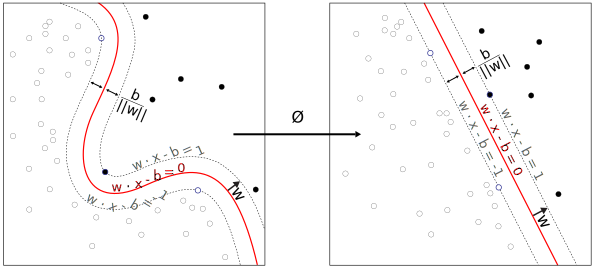
\includegraphics[width=\textwidth,height=\textheight,keepaspectratio]{../Chap3/Figures/Kernel_Machine_Pierre.pdf}
    \caption{SVM avec \emph{kernel trick} $\varphi$. Figure originale de \href{https://commons.wikimedia.org/wiki/File:Kernel_Machine.png}{Alisneaky \ccLogo \ \textnormal{0}, Wikimedia Commons}.}
    \label{fig:svm}
\end{figure}

La librairie \textit{LIBSVM} \cite{chang_libsvm_2011} permet de résoudre le problème avec différents noyaux non linéaires, dans un ordre de grandeur de $\bigO(N^2)$ à $\bigO(N^3)$.
Aussi, elle n'est plus utilisable lorsque le nombre d'échantillon dépasse dix mille.
Dans nos travaux, nous utilisons la librairie \textit{LIBLINEAR} de \cite{fan_liblinear_2008}, au travers de l'interface de la libraire \textit{SciKit-Learn} \cite{pedregosa_scikit-learn_2011}.
La complexité de l'apprentissage, avec des noyaux linéaires, est de l'ordre de $\bigO(N)$, avec $N$ le nombre d'échantillons ce qui rend cette méthode intégrable sur des systèmes embarqués modernes aux vues des puissances de calculs aujourd'hui disponibles.
L'apprentissage d'un modèle peut être effectué pendant le cycle de production et le système de calcul peut être intégré directement au cœur de l'atelier de production, au plus près du procédé d'injection-moulage.

\paragraph{K-plus-proches voisins} \mbox{} \label{parag:knn} \\
La méthode des k-plus-proches voisins a été proposée par \cite{fix_discriminatory_1951} et développée par \cite{cover_nearest_1967}.
Cette méthode est à l'origine de méthodes d'apprentissages non supervisées, par exemple celles basées sur les variétés et l'analyse spectrale.
Cette méthode ne cherche pas à construire de modèle générique au problème de classification.
Elle enregistre les positions des échantillons du jeu d'apprentissage dans l'espace des données.
La classification d'un nouvel échantillon est la classe majoritaire sur l'ensemble des échantillons parmi les $k$ plus proches voisins.
Le nombre de voisins $k$ peut être prédéfini ou bien varier à partir de la densité  de points (la métrique de distance entre points est souvent la norme Euclidienne $\ell_{2}$).
Cette méthode est particulièrement efficace lorsque la séparation entre les échantillons est irrégulière.

%\paragraph{Régression logistique}\mbox{} \\
%TODO

\paragraph{Bagging}\mbox{\label{parag:bagging}} \\
Le \textit{bagging} (\textit{\emph{B}ootstrap \emph{agg}regat\emph{ing}}) est une méthode d'association ensembliste de modèles simples afin d'obtenir un méta-modèle aux performances supérieures.
Il est défini par \cite{breiman_bagging_1996}.
La technique permet de limiter le sur-apprentissage.
Pour un jeu de données $\mathbf{X}$ de taille $n$, on génère $b$ lots $\mathbf{X}_b \in \mathbf{X}$ contenant $\sim 10 < m < n$ échantillons tirés aléatoirement selon une distribution uniforme.
Les échantillons, uniques dans $X$, peuvent être répétés dans $\mathbf{X}_b$.
Pour chaque lot $b$, un modèle de l'algorithme choisi est entrainé.
La prédiction du méta-modèle final est la moyenne (ou le vote pondéré) de tous les modèles $f_b$, Équation \ref{eq:bagging}.
Cette méthode d'agrégation de modèles est efficace pour limiter le sur-apprentissage.
La méthode est employée dans les \textit{Random Forests} et elle est souvent combinée avec le \textit{boosting} \ref{parag:boosting}.
La méthode de référence pour calculer le nombre optimal $b$ de fonctions est la sélection du meilleur score par validation croisée \ref{subsubsec:cross_val}.

Une métrique intéressante se base sur la performance individuelle de chaque modèle $f_b$ vis à vis de son jeu de données partiel $\mathbf{X}_b$.
\cite{breiman_bagging_1996} définit l'erreur \textit{Out-of-Bag} comme la moyenne, de l'erreur de prédiction pour chaque échantillon $\mathbf{x}_{i,\bar{b}}$, des modèles $f_b$ avec $ \mathbf{x}_{\bar{b}} \notin \mathbf{X}_b$ qui n'ont pas été entrainés avec les échantillons $x_i$.
Cette erreur est similaire à une erreur de prédiction qui serait calculée sur des échantillons de validation.
Elle permet ainsi de se passer de jeu de données de validation.
Elle est utilisé par les \textit{Random Forests} \ref{parag:random_forests} pour mesurer l'influence des variables sur la prédiction.

\begin{equation} \label{eq:bagging}
f_{boosted} = \frac{1}{b} \sum_{b=1}^{b} f_{b}\left(x_b\right)
\end{equation}

\paragraph{Forêt d'arbres décisionnels}\mbox{\label{parag:random_forests}} \\
L'arbre décisionnel est une méthode de classification adaptée au grands jeux de données.
Un arbre se compose de branches avec entre chacune d'elle un nœud.
Chaque nœud répond à une condition sur une variable d'entrée.
Ainsi, le modèle obtenu peut être facilement interprété par l'humain.
Le modèle obtenu est cependant peu robuste aux perturbations des variables d'entrée.
La complexité du modèle est souvent égale au nombre de variables d'entrée ce qui est une cause de sur-apprentissage.
Son utilisation pour des échantillons d'entrée qui comporte une dimension supérieure à dix mille est difficile (par exemple les pixels d'une image).
C'est pourquoi \cite{ho_random_1995, ho_random_1998} propose un modèle comportant de multiples arbres de décisions (une forêt), chacun entrainés sur une unique partie des variables des échantillons.
La prédiction du modèle est donnée par la moyenne des prédictions de l'ensemble des arbres. 
\cite{breiman_random_2001} fait évolué la méthode : les arbres sont choisis pour ne pas être corrélés entre eux et leurs sorties sont agrégées par \textit{bagging} \ref{parag:bagging}.

Une utilité indirecte de la notion stochastique des forêts d'arbres décisionnels est la possibilité de mesurer l'influence des variables sur le modèle.
Lors de l'entrainement, l'erreur \textit{Out-of-Bag} \ref{parag:bagging} (équivalente à une erreur de prédiction sur un échantillon de validation) est moyennée pour l'ensemble des arbres.
C'est l'erreur \textit{Out-of-Bag} de référence, pour chacune des variables $j$, $e_{ref, j}$.
À chaque itération, on permute aléatoirement la position des variables $v$ dans le jeu de données et on calcule à nouveau l'erreur \textit{Out-of-Bag}.
Les permutations sont réalisées un grand nombre de fois ($p > 1000$).
On obtient l'importance de la $j^{\text{ième}}$ variable en calculant la moyenne de l'erreur sur toutes les permutations $\bar{e_{perm}}$ de la différence avec l'erreur de référence de la variable : $importance_{j} = \bar{e_{perm, j}} - e_{ref, j}$.
Il est enfin possible de normaliser la valeur de l'importance par l'écart-type sur l'ensemble des variables pour classer les variables sur une échelle continue $[0 ; 1]$.
Nous utiliserons cette méthode pour sélectionner les variables pertinentes.

\paragraph{Boosting}\mbox{\label{parag:boosting}} \\
\cite{kearns_thoughts_1988} pose l'hypothèse de l'existence d'un méta-classifieur qui utiliserait une association de classifieurs aux performances non optimales (légèrement supérieure à une réponse aléatoire) pour obtenir de bonnes performances : le \textit{boosting}.
Dans un tel ensemble, chaque classifieur est ainsi faiblement corrélé avec la totalité des données.
\cite{schapire_strength_1990} vérifie l'hypothèse et par la suite \cite{breiman_bias_1996, breiman_arcing_1997} développe la méthode.
De nombreux algorithmes sont dérivés de cette méthode.
Par la suite, \cite{mason_boosting_1999, friedman_greedy_2001} propose le \textit{boosting} avec descente de gradient (\textit{Gradient Boosting}) et \cite{friedman_stochastic_2002} ajoute une dimension stochastique : \textit{Stochastic Gradient Boosting}.
Cette idée est motivée par le \textit{bagging} \ref{parag:bagging}.
Chaque classifieurs est entrainé sur des partitions aléatoires différentes du jeu de données, mais sans aucune répétition des échantillons initiaux.
Une partition qui a pour dimensions la moitié du jeu de données initial produit une augmentation de performance significative du méta-classifieur.
Un des algorithmes le plus populaire dans des compétitions de classification est \textit{XGBoost}.
Il est basé sur le \textit{Stochastic Gradient Boosting} d'arbres de décisions binaires.
Cependant, les performances de cet algorithme pour des jeux de données où les échantillons possèdent de grandes dimensions ($> 1000$), comme des images, sont inférieures aux méthodes à réseaux de neurones profonds.
La performance de ces algorithmes dépendent de la pertinence de la réduction de la dimension des échantillons, qui doit être implémentée par un humain.
Les réseaux de \textit{Deep Learning} dépassent cette limite en apprenant l'algorithme de réduction de dimensions adapté en même temps que l'algorithme de classification.
Enfin, les idées issues du \textit{bagging} et du \textit{boosting} sont utilisées dans les méthodes d'apprentissages des réseaux de neurones profonds.

\paragraph{Réseaux de neurones}\mbox{} \label{parag:neural_networks} \\
Le travail de \cite{mcculloch_logical_1943} interroge sur la méthode de fonctionnement du cerveau humain : de nombreuses cellules élémentaires connectées entre elles permettent de résoudre des problèmes complexes, ce qui pose la problématique de la recherche Connexionniste.
Ils proposent de concevoir des neurones, sous la forme de portes logiques élémentaires.
Pour des valeurs d'entrée $\mathbf{x}_i$, un neurone calcule la somme pondérée par une matrice de poids $\mathbf{W}$, puis si la valeur obtenue est supérieure à une valeur $b$, la sortie est zéro, sinon la sortie est un, Équation \ref{eq:perceptron}.
Cet algorithme permet de convertir des variables continues en valeurs booléennes discontinues.
Par la suite, \cite{rosenblatt_perceptron_1958} propose le \textit{perceptron}, en s'appuyant sur la connaissance de l'époque du système de la vision biologique : de la rétine au cerveau.
Le \textit{perceptron} permet d'agréger à l'aide d'un réseau de neurones à une couche, des données représentant des variables pertinentes extraites d'images (\textit{pre-processing}).
La thématique de recherche Connexionnisme sera peu développée par la suite car les ressources informatiques nécessaires sont importantes et les résultats obtenus sont limités en comparaison des attentes de l'époque.
Les autres méthodes présentées dans cette section seront préférées, jusqu'aux récents succès du \textit{Deep Learning}, §\ref{subsubsec:deep_learning}.

\begin{equation} \label{eq:perceptron}
f_{perceptron}(x_i)=\left\{\begin{array}{ll}{1} & {\text { si } \mathbf{w}_i \cdot x_i + b_i > 0} \\ {0} & {\text { sinon }}\end{array}\right.
\end{equation}

Suite à la proposition de réseaux de neurones à multiples couches successives \cite{fukushima_neocognitron_1980}, \cite{rumelhart_learning_1985} applique une méthode d'ajustement itératif des poids en utilisant la rétro-propagation de l'erreur.
La rétro-propagation de l'erreur s'appuie sur les travaux sur la dérivation automatique des fonctions composées, initiés par \cite{linnainmaa_taylor_1976}.
De plus, \cite{rumelhart_learning_1985} étend les capacités du réseau à répondre aux problèmes où les données ne sont pas linéairement séparables, en introduisant des fonctions d'activations non linéaires, en lieu et place de la simple condition inférieure/supérieure.
La particularité des réseaux de neurones est leur capacité à modéliser des problèmes fortement non linéaires.
La prochaine étape est la construction de réseaux aux architectures plus complexes et l'utilisation de fonctions de convolution, §\ref{subsubsec:deep_learning}.

\subsubsection{Réseaux profonds de convolutions, Deep Learning} \label{subsubsec:deep_learning}
Les réseaux de neurones de convolutions, proposés par \cite{lecun_backpropagation_1989}, ont un comportement non linéaire particulièrement adapté à l'analyse de données complexes, telles que des images, et à l'apprentissage de représentations de ces données.
La couche de convolution est l'élément principal du réseau.
Les couches de convolutions sont associées les unes à la suite des autres pour former un réseau profond (d'où le nom de \textit{Deep Learning}).
Entre chaque couche peuvent être ajoutées des couches composées de fonctions d'activations non linéaires, des couches de moyennes globales ou locales, ou d'autres fonctions avancées.
Le réseau résultant est une composée de fonctions de convolutions avec des fonctions intermédiaires.
L'Équation \ref{eq:deep_function} détaille la forme d'un modèle complet $F$ et de l'application d'une couche $f_n$ : c'est un modèle affine composé d'une matrice de poids $\mathbf{W}$ et d'un vecteur de biais $\mathbf{b}$.

\begin{equation} \label{eq:deep_function}
F(\mathbf{x}) = \left(f_{n} \circ f_{n-1} \circ \ldots f_{2} \circ f_{1}\right)(\mathbf{x}), \ \text{avec} \ f_n(\mathbf{x}) = \mathbf{w}_n \cdot \mathbf{x} + \mathbf{b}_n
\end{equation}

De plus, l'opération de convolution est très efficiente pour des problèmes en grandes dimensions \cite{goodfellow_deep_2016}.
Pour une entrée de dimensions $m$, et une sortie de dimensions $n$, l'application matricielle complète $x \rightarrow y$ aura une complexité $\bigO(m \cdot n)$.
L'opération de convolution pour un noyau de dimensions $k$ aura une complexité de $\bigO(k \cdot n)$.
Lorsque la dimension du noyau $k$ est très petite devant la dimension de l'entrée $m$, l'opération de convolution permet un gain d'occupation mémoire et ainsi de coût de calcul.
Le gain est considérable lorsque les données d'entrée ont de grandes dimensions, comme dans notre cas avec des images.
Il est bien plus efficient de créer des architectures profondes, supérieures à $c$ couches de convolutions successives avec des noyaux de petite dimension $k$, car $c$ est très petit devant $m$.

Ces réseaux ont profité de la disponibilité croissante de la puissance de calcul des processeurs graphiques.
En 2006, le premier réseau de convolution est implémenté sur processeur graphique \cite{chellapilla_high_2006}, avec des performances quatre fois supérieures à l'implémentation sur processeur classique.
En 2011, un réseau de convolution accéléré sur processeur graphique (60 fois plus rapide) dépasse les performances de l'humain sur une tâche de classification de panneaux signalétiques routiers \cite{ciresan_flexible_2011}.
En 2012, le réseau AlexNet \cite{krizhevsky_imagenet_2012} gagne le challenge annuel de classification d'images \textit{ImageNet} \cite{deng_imagenet_2009} avec un très grand écart de 10,8\% sur le score, avec l'ensemble des concurrents.
La performance d'\textit{AlexNet} (8 couches) est dépassée en 2013 par \cite{zeiler_visualizing_2013} une version identique aux hyper-paramètres optimisés, puis en 2014 par \textit{VGG16-19} \cite{simonyan_very_2014} (16 et 19 couches) et \textit{GoogleNet} (22 couches).
Ce dernier est dépassé en 2015, par le réseau \textit{ResNet101} \cite{he_deep_2015} contenant plus de 150 couches.
L'architecture massive de ces réseaux évolue depuis 2011 vers des architectures de plus en plus profondes \cite{he_deep_2015} et qui sont plus efficientes sur le plan de la mémoire à allouer et puissances de calculs, mais aussi de plus en plus complexes, §\ref{subsubsec:ResNet}.
Les architectures de l'état de l'art de la littérature dépassent aujourd'hui les capacités d'ingénierie humaine ; elles sont générées automatiquement, §\ref{section:auto_ml}.
La dernière couche du réseau est appelée couche de classification (ou classifieur).
Si le problème est binaire (comporte uniquement deux classes), la sortie du réseau est une probabilité d'appartenance à la première classe.
Pour un problème multi-classes, la sortie du réseau est un vecteur de probabilité d'appartenance à chacune des classes.
Pour un problème binaire, une fonction d'activation sigmoïde, Équation \ref{eq:sigmoid}, est utilisée afin de transformer les valeurs de la précédente couche vers une probabilité : $s_{[-\infty; +\infty]} \to p_{[0 ; 1]}$.

\begin{equation} \label{eq:sigmoid}
\text{Sigmoïde} \ \ \ f\left(s_{i}\right)=\frac{1}{1+e^{-s_{i}}}
\end{equation}

Pour un problème multi-classes, une fonction \textit{SoftMax} (Équation \ref{eq:softmax}), inverse de la sigmoïde, est utilisée.
$\text{SoftMax} = \vec{s}_{[-\infty; +\infty]} \to \vec{p}_{[0 ; 1]}$
Chaque classe a préalablement été encodée sous la forme d'un vecteur à la dimension égale au nombre total de classes, c'est le \textit{one-hot encoding}.

\begin{equation} \label{eq:softmax}
\text{SoftMax} \ \ f(s_{i})=\frac{e^{s_{i}}}{\sum_{c}^{nb \ classes} e^{s_{c}}}
\end{equation}


Ce modèle à réseau de neurones est pleinement différentiable. C'est pourquoi la méthode traditionnelle d'ajustement des poids des neurones du réseau est la rétro-propagation de l'erreur proposée, par \cite{rumelhart_learning_1985} qui est adaptée aux réseaux de convolutions à couches multiples par \cite{lecun_backpropagation_1989}.
Par la suite, \cite{lecun_efficient_1998} développe l'apprentissage progressif stochastique des poids du réseau, aussi appelée descente de gradient stochastique : l'apprentissage est réalisé successivement sur une portion des données choisie aléatoirement  (les \textit{mini-batch}), car  calculer le gradient pour la totalité du jeu de données serait trop coûteux en matière de puissance de calcul.

\cite{vapnik_principles_1992} définit dans la théorie Vapnik–Tchervonenkis la notion d'apprentissage statistique comme un problème d'optimisation, Équation \ref{eq:VC_error}, où on cherche à minimiser l'erreur empirique $E$, en fonction des poids $\mathbf{W}$ du réseau et d'un terme de régularisation $\lambda$ sur les poids $\mathbf{W}$ (régularisation de Tikhonov §\ref{parag:weights_decay}).

\begin{equation} \label{eq:VC_error}
E\left(\mathbf{W}, \lambda_{p}\right)=\frac{1}{\ell} \sum_{i=1}^{\ell} L\left(y_{i}, f\left(x_{i}, \mathbf{W}\right)\right)+\lambda_{p}\|\mathbf{W}\|_{2}
\end{equation}

A chaque itération, une fonction de coût $\mathcal{L}$ calcule l'erreur entre les prédictions du réseau $\hat{y}$ et les valeurs de références $y$.
La fonction de coût est choisie pour être adaptée au problème de classification en présence.
Nous détaillerons dans ce paragraphe le cas de la classification binaire.
L'entropie $H$ est une métrique importante de la théorie de l'information, proposée par \cite{shannon_mathematical_1948}.
Pour une distribution de probabilité $p$ donnée, l'entropie est exprimée par l'Équation \ref{eq:entropy}.
Elle mesure la quantité de données minimale nécessaire pour encoder l'information de la distribution.

\begin{equation} \label{eq:entropy}
\text{Entropie} \ \ H(p) =-\sum_{i=1}^{N} p\left(x_{i}\right) \cdot \log p\left(x_{i}\right)
\end{equation}

Dans le cas de l'apprentissage supervisé, on cherche à trouver la fonction $F$ qui minimise la perte de l'information entre l'approximation finale et le jeu de données initial.
Aussi, en comparant les entropies d'une distribution source $y$ et d'une approximation de $\hat{y}$, on mesure la quantité d'informations, perdue par la méthode d'approximation $F$ apprise (aussi appelée méthode d'encodage).
C'est la divergence de Kullback-Leibler \cite{kullback_information_1951}, Équation \ref{eq:D_KL} et nous cherchons ici à la minimiser.

\begin{equation} \label{eq:D_KL}
Divergence_{K L}(y \| \hat{y})=\sum_{i=1}^{N} y\left(\mathbf{x}_{i}\right) \cdot\left(\log y\left(\mathbf{x}_{i}\right)-\log \hat{y}\left(\mathbf{x}_{i}\right)\right)
\end{equation}

Dans le cas d'une classification binaire, on utilise ainsi la fonction de coût logistique (Équation \ref{eq:bce_loss}), aussi appelée entropie-croisée binaire. Cette fonction est généralisable aux problèmes multi-classes avec $i > 1$.

\begin{equation} \label{eq:bce_loss}
\mathcal{L}_{logit}\left(\hat{y}, y\right) = -\sum^{2}_{i=1} y_{i} \log \left(\hat{y_{i}}\right) = - y_{1} \log \left(\hat{y_{1}}\right) -\left(1-y_{1}\right) \log \left(1-\hat{y_{1}}\right)
\end{equation}

Le calcul est simplifié en combinant la fonction d'activation sigmoïde et la fonction de coût logistique, Équation \ref{eq:bce_loss_simple}.

\begin{equation} \label{eq:bce_loss_simple}
\begin{split}
\left(\mathcal{L}_{logit} \circ f_{sig}\right)\left(X, y_{1}\right) = - y_{1} \log \left(f_{sig}(X)\right) -\left(1-y_{1}\right) \log \left(1-f_{sig}(X)\right) = -y_1 \cdot X +\log \left(1+e^{X}\right)
\\
\text{d'où} \ \ \left(\mathcal{L}_{logit} \circ f_{sig}\right)\left(X, y_{1}\right) = \left\{\begin{array}{cc}{- X +\log \left(1+e^{X}\right)} & {\text { si } y_{1}=1} \\ {\log \left(1+e^{X}\right)} & {\text { si } y_{1}=0}\end{array}\right\}
\end{split}
\end{equation}

A chaque itération, la dérivée de cette erreur est rétro-propagée pour ajuster chacun des poids du réseau.
Le lecteur pourra se référer à \cite{sadowski_notes_2016} pour le détail du calcul de la dérivée.
De plus, la dérivée est pondérée par un facteur $0 < \eta < 1$ qui est appelée le facteur d'apprentissage.
Le facteur $\eta$ est critique pour obtenir la convergence de l'erreur vers zéro.
Plus le réseau est complexe, plus le problème d'optimisation en présence est non-linéaire et non-convexe ; il possède de nombreux minima locaux.
C'est pourquoi, un facteur $\eta$ trop petit demandera un grand nombre d'itérations avant d'obtenir la convergence et l'équilibre sera souvent atteint sur un minima local.
A contrario, un facteur $\eta$ trop grand empêchera la convergence car le gradient oscillera.
Les deux problèmes critiques à éviter lors de l'ajustement par descente de gradients sont l'effondrement du gradient qui occasionne une convergence globale des poids du réseau vers zéro et l'explosion du gradient qui occasionne une divergence globale des poids du réseau vers l'infini \cite{bengio_learning_1994, hochreiter_gradient_2001}.
Des algorithmes avancés existent pour limiter ces problèmes.
La vaste littérature sur le sujet ne nous permettra pas de détailler l'intérêt des différentes méthodes proposées, aussi, nous utiliserons dans l'ensemble de nos travaux l'algorithme d'optimisation récent \textit{Adam} proposé par \cite{kingma_adam_2014}.

Ce dernier permet l'ajustement automatique du facteur d'apprentissage  $\eta$ au fur et à mesure des itérations.
De plus, des facteurs de régularisation sur la dérivée seconde (aussi appelé "moment") sont ajoutés pour accélérer la convergence et éviter les minimums locaux.

Nous récapitulons dans le Tableau \ref{tab:cnn_hyperparameters} les différents hyper-paramètres critiques de l'apprentissage par descente de gradient stochastique des réseaux de neurones profonds. Dans ce travail, nous ne présenterons pas de manière exhaustive les contraintes qui existent sur l'architecture des réseaux de convolutions. Le choix des nombres de couches, des dimensions des noyaux de convolutions, des décalages, remplissages (\textit{padding}), réduction (\textit{pooling}, §\ref{parag:pooling}). Nous invitons le lecteur à se référer à l'excellente synthèse \cite{dumoulin_guide_2016}.

\begin{table}[]
    \centering
    \begin{tabular}{|l|c|l|}
        \hhline{---}
        Hyper-paramètres         & Valeurs de la littérature         & Description  \\
        \hhline{=:=:=} %\hline
        Nombre de couches        & $[2 ; 200]$                       & Nombre de couches dans le réseau.  \\ \hline
        Type de couche           & Convolution, Connectés, Pooling & Type de couche, varie à chaque couche.  \\ \hline
        Neurones par couche      & $[1 ; 4000]$                      & Varié à chaque couche successive.  \\ \hline
        Fonction d'activation    & tanh, sigmoïde, SoftMax           & Transforme la sortie en probabilités.  \\ \hline
        Fonction de coût         & Logistique, Entropie-croisée, $\ell_{1}$, $\ell_{2}$ & Erreur entre  référence et prédiction. \\ \hline
        Initialisation           & Loi uniforme, normale …           & Méthode d’initialisation des poids.  \\ \hline
        Régularisation des poids & $\ell_{1}$, $\ell_{2}$                            & Limite l’explosion des poids.  \\ \hline
        Facteur d’apprentissage  & $[10^{-7} ; 10^{-1}]$             & Pas du gradient, vitesse de convergence.  \\ \hline
        Lots d'apprentissage/\textit{mini-batch}  & $[16 ; 128]$                      & Nombre d'échantillons par lot  \\
        \hhline{---}
    \end{tabular}
    \caption{Hyper-paramètres critiques pour l'apprentissage de réseaux de neurones profonds.}
    \label{tab:cnn_hyperparameters}
\end{table}

Dans ce travail, nous avons étudié un panel représentatif de différentes architectures récentes de réseaux de neurones profonds, sur notre cas d'application de contrôle de la qualité.
Le Tableau \ref{tab:deep_models} présente les architectures étudiées avec leurs occupations de mémoire de travail, le nombre de paramètres (Degrés De Libertés) et les scores de justesse obtenus sur le jeu de données de validation d'\textit{ImageNet}.
L'erreur \textit{Top-1\%} correspond à l'erreur de justesse pour l'annotation qui est prédite avec la plus grande probabilité par le réseau.
L'erreur \textit{Top-10} correspond à l'erreur de justesse pour les dix annotations qui sont prédites avec la plus grande probabilité par le réseau.
Ainsi, si l'annotation qui devait être prédite est "chat", mais que le réseau prédit l'annotation "chat" en neuvième position, alors l'erreur \textit{Top-10\%} sera nulle, mais l'erreur \textit{Top-1} sera maximale.
Dans notre problématique de classification binaire de la qualité, nous nous intéressons uniquement à l'erreur \textit{Top-1}.
Nous distinguons également les ressources informatiques nécessaires à entrainer ces modèles : la durée du calcul et la mémoire de travail nécessaire.
De plus, pour réaliser l'inférence à l'aide de ces modèles, ils doivent être chargés en mémoire de travail (\textit{RAM} du processeur, ou \textit{RAM} du \textit{GPU}).
Les modèles qui possèdent un grand nombre de poids nécessitent de grandes quantités de mémoires ce qui limite leur utilisation dans des systèmes embarqués positionnés au cœur des ateliers de production.
La faible quantité de données annotées dont nous disposons est une problématique industrielle qui a orienté nos travaux vers le transfert de modèles profonds, préalablement appris sur de grandes quantités de données annotées, §\ref{subsec:transfer_learning}.

\begin{table}[]
    \centering
    \arrayrulecolor{black}
    \begin{tabular}{|l|r|r|r|r|r|r|}
        \hhline{------}
        Architecture             & Année & Mémoire & Paramètres & Erreur Top-1\% & Erreur Top-5\% \\
        \hhline{=:=:=:=:=:=} %\hline
        MobileNetV2              & 2018  & 14 Mo   & 3,5 M      & 28,12          & 9,71           \\ \hline
        VGG19                    & 2014  & 549 Mo  & 143,6 M    & 25,76          & 9,12           \\ \hline
        DenseNet-201             & 2016  & 80 Mo   & 20,2 M     & 22,80          & 6,43           \\ \hline
        ResNet-152               & 2015  & 232 Mo  & 60,3 M     & 21,69          & 5,94           \\ \hline
        ResNext-50\_32x4d        & 2016  & 85 Mo   & 25,1 M     & 22,38          & 6,30           \\ \hline
        ResNext-101\_32x8d       & 2016  & 170 Mo  & 44,3 M     & 20,69          & 5,47          \\ \hline
        ResNeXt-101\_32x48d\_wsl & 2018  & 3100 Mo & 829 M      & 14,6           &     2,4           \\
        \hhline{------}
    \end{tabular}
    \caption{Architecture des réseaux de convolutions étudiés.}
    \label{tab:deep_models}
\end{table}

\subsubsection{Réseaux de convolutions résiduels} \label{subsubsec:ResNet}
Construire des réseaux de neurones aux architectures profondes permet de limiter l'utilisation de couches pleinement connectées, dont les poids sont très coûteux à optimiser.
La problématique principale des réseaux profonds est l'entrainement.
La rétro-propagation a une faible incidence sur les poids situés les plus en amont du réseau.
Cela rend l'entrainement des réseaux aux couches supérieures à dix très difficile.
C'est pourquoi des connections intermédiaires ont été introduites par \cite{srivastava_highway_2015, srivastava_training_2015} : les \textit{Highway Networks}.
Elles permettent à la rétro-propagation d'agir sur toutes les couches, y compris les couches en amonts.
Cette architecture est inspirée des connections intermédiaires pondérées des réseaux récurrents \textit{Long Short-Term Memory}.
Soit $y_{i+1}$ la sortie d'une couche $i$ qui est composée d'une fonction affine et d'une activation non linéaire $f_{i+1}$ dont les poids sont $\mathbf{W}_f$.
On introduit une connexion intermédiaire $T$ pondérée par une matrice de poids $\mathbf{W}_T$, Équation \ref{eq:highway}.
Le poids $\mathbf{W}_T$ détermine si la couche laissera passer l'information ou la transformera.
Les auteurs notent que $\mathbf{W}_T$ doit être initialisée à des valeurs négatives afin de débuter nécessairement l'apprentissage de $\mathbf{W}_f$.
Par la suite, $f$ pourra être ignoré au fur et à mesure de l'apprentissage si cela entraine de meilleures performances.
De manière simplifiée, cette architecture permet au réseau d'ajuster sa profondeur optimale, lors de l'apprentissage : si les connections intermédiaires sont utilisées, le réseau est moins profond.

\begin{equation} \label{eq:highway}
y_{i+1} = f_{i+1}\left(y_{i}, \mathbf{W}_f\right) \cdot T_{i+1}\left(y_{i}, \mathbf{W}_{T}\right)+y_{i} \cdot \left(1- T_{i+1}\left(y_{i}, \mathbf{W}_{T}\right)\right)
\end{equation}
%TODO: plot highway cell

Par la suite, \cite{he_deep_2015} propose l'architecture \textit{ResNet} qui est un cas particulier de \textit{Highway Network} où $\mathbf{W}_T \equiv 0,5$, Équation \ref{eq:resnet}.
Les données sont transmises de manière équivalente entre la transformation et la connexion intermédiaire.
\cite{he_identity_2016} compare les performances des deux méthodes et montre que la plus simple architecture \textit{ResNet} offre de meilleures performances.
Cependant, \cite{srivastava_highway_2015} montre que la valeur apprise de $\mathbf{W}_t$ est différentes de $0.5$.
On a particulièrement souvent $\mathbf{W}_T > 0.5$ : le réseau a appris à utiliser en priorité les connections intermédiaires, ce qui simplifie le réseau mais impacte les performances.
De plus, les poids $\mathbf{W}_T$ augmentent le nombre de paramètres à apprendre, ce qui pourrait diminuer la performance.

\begin{equation}\label{eq:resnet}
y_{i+1} = f_{i+1}\left(y_{i}, \mathbf{W}_f\right)+y_{i}
\end{equation}
%TODO: plot resnet cell

Par la suite, ces idées amènent à l'architecture \textit{DenseNet} \cite{huang_densely_2016} : les connections intermédiaires sont présentes entre toutes les couches et non plus seulement d'une couche à l'autre.
Toutes les couches peuvent alors avoir accès à l'information de bas niveau, comme par exemple l'image originale et combiner cette information pour résoudre le problème.
La Figure \ref{fig:densenet} présente l'architecture d'un bloc \textit{Dense}.
\footnote{Les architectures présentées dans ce travail sont générées avec l'aide des scripts développés par \cite{harisiqbal_harisiqbal88_2018}.}
Un réseau complet enchaine successivement quatre blocs \textit{dense}.

\begin{figure}[hbtp]
    \centering
    \includegraphics[width=\textwidth,height=\textheight,keepaspectratio]{../Chap3/Figures/densenet.pdf}
    \caption{Architecture d'un bloc DenseNet.}
    \label{fig:densenet}
\end{figure}

La dernière évolution des réseaux résiduels est l'introduction de multiples blocs dans chaque neurones classiques.
C'est l'architecture \textit{ResNext} \cite{xie_aggregated_2016}, une dimension $C$ dite de "cardinalité" qui définit le nombre de bloc présent dans chaque couche. Les auteurs montrent l'intérêt d'une architecture où $c = 32$ : chaque bloc est répété 32 fois par neurones. 

Les performances sont améliorées bien que cela représente une augmentation conséquente des paramètres du réseau.
Dernièrement, \cite{mahajan_exploring_2018} a réussi à augmenter les performances sur \textit{ImageNet} en réalisant un pré-apprentissage sur 940 millions d'images issues d'\textit{Instagram}.
La capacité (au sens de la théorie VC \cite{vapnik_principles_1992}) du modèle \textit{ResNext} est bien supérieure à la seule base \textit{ImageNet} et un plus grand nombre de données réelles permet d'augmenter les performances, par la généralisation du problème.

Cependant, l'augmentation du nombre de paramètres des réseaux n'est pas nécessairement significative de meilleures performances.
Dernièrement, le réseau \textit{EfficientNet} dépasse l'état de l'art sur \textit{ImageNet} en diminuant drastiquement le nombre de paramètres ajustables et optimisant sous contrainte l'occupation mémoire et le nombre d'opérations nécessaires.
Précédemment, les réseaux \textit{MobileNetV1} \cite{howard_mobilenets_2017} et \textit{MobileNetV2} \cite{sandler_mobilenetv2_2018} cherchent à obtenir les meilleures performances sur dispositifs embarqués tels que les smartphones.
Il s'agit de limiter le nombre de paramètres et le nombre d'opérations à réaliser (additions et multiplications).
\textit{MobileNetV1} obtient une performance supérieure à \textit{GoogLeNet}, avec trois fois moins d'opérations à réaliser.
Il égale \textit{VGG19} avec trente fois moins d'opérations et d'occupation mémoire.
\textit{MobileNetV1} utilise un bloc de convolution efficient, proposé dans l'architecture \textit{Xception} \cite{chollet_xception_2016} : la convolution est effectuée indépendamment sur chaque canal, avec un poids différent pour chaque canal, puis les résultats sont concaténés.
Pour une convolution traditionnelle de fenêtre $3 \times 3$, la réduction du nombre d'opérations de calcul à effectuer est d'un facteur $9$.
\textit{MobileNetV2} ajoute ensuite l'utilisation de connexions intermédiaires entre chaque couche, à la manière des réseaux résiduels.
Les performances de ces réseaux sont inférieures à l'état de l'art mais ils permettent d'exécuter l'inférence avec des performances satisfaisantes sur des systèmes embarqués.
%TODO: plot deepwise conv
% https://arthurdouillard.com/post/3-small-but-powerful-cnn/
% https://medium.com/@yu4u/why-mobilenet-and-its-variants-e-g-shufflenet-are-fast-1c7048b9618d

\subsubsection{Fonctions d'activations} \label{subsubsec:activation}
Pour éviter les deux problèmes de l'explosion ou de l'effondrement de la valeur du gradient pendant l'apprentissage, nous utiliserons dans nos travaux des fonctions d'activation \textit{LeakyReLU}, \textit{PreLU} ou \textit{ELU}, récemment proposées dans la littérature.
La fonction d'activation est une non-linéarité qui suit traditionnellement l'opération de convolutions.
Elle permet de modéliser une réponse à un problème non linéaire.
Les fonctions d'activation historiques sont la tangente hyperbolique et la sigmoïde.
\cite{nair_rectified_2010} propose la fonction \textit{ReLU} (\textit{Rectified Linear Unit}) qui une approximation de la sigmoïde par trois et obtient de meilleures performances, en diminuant le coût du calcul.

\begin{table}[]
    \centering
    \setlength{\tabcolsep}{2em} % for the horizontal padding
    \renewcommand{\arraystretch}{1.5}% for the vertical padding
    \begin{tabular}{|l|l|l|}
        \hline
        Fonction  & Équation                                                                                                                 & Dérivée                                                                                                            \\ \hline\hline
        Sigmoïde  & $f(x) = \frac{1}{1+e^{-x}}$                                                                                                     & $f(x)(1-f(x))$                                                                                                     \\ \hline
        Tanh      & $tanh(x)  = \frac{2}{1+e^{-2 x}}-1$                                                                                      & $1-f(x)^{2}$                                                                                                       \\ \hline
        ReLU      & $\left\{\begin{aligned} {0} & {\text { si } x<0} \\ {x} & {\text { si } x \geq 0}\end{aligned}\right.$                    & $\left\{\begin{aligned} {0} & {\text { si } x<0} \\ {1} & {\text { si } x \geq 0}\end{aligned}\right.$              \\ \hline
        LeakyReLU & $\left\{\begin{aligned} 0,01 x & \text { si } x<0 \\ x & \text { si } x \geq 0 \end{aligned}\right.$                     & $\left\{\begin{aligned}{0,01} & {\text { si } x<0} \\ {1} & {\text { si } x \geq 0}\end{aligned}\right.$     \\ \hline
        PreLU     & $\left\{\begin{aligned} \alpha x & \text { si } x<0 \\ x & \text { si } x \geq 0 \end{aligned}\right.$                   & $\left\{\begin{aligned}{\alpha} & {\text { si } x<0} \\ {1} & {\text { si } x \geq 0}\end{aligned}\right.$ \\ \hline
        ELU       & $\left\{\begin{aligned} \alpha\left(e^{x}-1\right) & \text { si } x<0 \\ x & \text { si } x \geq 0 \end{aligned}\right.$ & $\left\{\begin{aligned} f(x)+\alpha & \text { si } x<0 \\ 1 & \text { si } x \geq 0 \end{aligned}\right.$          \\ \hline
    \end{tabular}
    \caption{Fonctions d'activation.}
    \label{tab:activations}
\end{table}

Le principal problème est que la fonction \textit{ReLU} vaut zéro pour des valeurs négatives.
C'est pourquoi \cite{maas_rectifier_2013} introduit le \textit{LeakyReLU} : une section de deux droites affines, dont la pente de la droite pour les valeurs négatives est non nulle, mais très faible ($0,01 \cdot x$).
Par la suite, \cite{he_delving_2015} introduit le \textit{PreLU} (\textit{Parametric ReLU}) dont un paramètre $\alpha \geq 0$ définit la pente de la droite pour les valeurs négatives.
$\alpha$ est appris au cours de l'apprentissage tout comme les matrices de poids du réseau.
La valeur de $\alpha$ peut également être indépendante pour chaque canal.
Ces fonctions sont discontinues et ne sont pas dérivables en zéro.
Cela peut entrainer des problèmes de convergence lors de la rétro-propagation du gradient.
C'est pourquoi dernièrement, \cite{clevert_fast_2015} propose le \textit{ELU} (\textit{Exponential Linear Unit}) qui est dérivable.
L'ensemble des graphes de ces fonctions est présenté dans la Figure \ref{fig:activation}, leurs dérivées dans le Tableau \ref{tab:activations}.

\begin{figure}[hbtp]
    \centering
    \includegraphics[width=0.7\textwidth,height=0.7\textheight,keepaspectratio]{../Chap3/Figures/activations.pdf}
    \caption{Fonctions d'activation.}
    \label{fig:activation}
\end{figure}
% https://www.mathcha.io/editor
% https://tikzcd.yichuanshen.de/

\subsubsection{Méthode de régularisation pour limiter le sur-apprentissage}
Le nombre de degrés de liberté d'un modèle à réseaux de neurones profonds est supérieur au million.
C'est pourquoi, il est courant que le modèle se spécialise afin d'obtenir un très bon score de justesse sur les échantillons d'apprentissages, mais un mauvais score sur de nouveaux échantillons : c'est le problème du \emph{sur-apprentissage}.
Plusieurs méthodes de régularisation permettent de limiter ce problème et nous détaillerons dans cette section les méthodes que nous utilisons.
\cite{goodfellow_deep_2016} propose une définition du terme "régularisation" spécifique à l'alchimie du \textit{Deep Learning} :
\begin{quote}
    « La régularisation est toute modification faite à un algorithme d'apprentissage afin que l'erreur de généralisation soit réduite, mais pas l'erreur d'apprentissage. »
\end{quote}

\paragraph{Dropout}\mbox{} \label{parag:dropout} \\
\cite{srivastava_dropout_2014} propose l'utilisation d'une couche dite de \textit{dropout} : la valeur de sortie de cette couche est aléatoirement, selon un pourcentage de chances $\alpha$ choisi, fixée à zéro. Le \textit{dropout} est actuellement la méthode de régularisation la plus performante pour limiter le sur-apprentissage.
Ainsi, l'optimisation est réalisée sur une mauvaise valeur (zéro) de sortie du modèle pour un pourcentage $\alpha$ d'échantillons d'un \textit{mini-batch}.
La valeur de $\alpha$ est souvent fixée entre $[0 ; 0,5]$.
Lors de l'utilisation du modèle pour inférence, la valeur de $\alpha$ est nulle : la couche de \textit{dropout} n'est jamais activée, pour ne pas fausser les prédictions.

\paragraph{Normalisation de lots}\mbox{} \label{parag:batchnorm} \\
La couche de normalisation de lots (\textit{Batch Normalization}) a été proposée par \cite{ioffe_batch_2015}.
Elle nécessite l'emploi de l'entrainement par descente de gradient stochastique qui découpe le jeu de données d'apprentissage en \textit{mini batch} répartis aléatoirement.
On définit les valeurs $x_i$ en entrée de la couche pour un \textit{mini batch} $B \in X$.
On calcule la variance $\sigma_B^2$ de l'entrée et la moyenne $\mu_B$.
La couche \textit{BN} normalise les valeurs des entrées $x_i$ en $\bar{x}_{i}$ par la variance et la moyenne de la distribution du \textit{mini batch}, Équations \ref{eq:batch_norm}.

\begin{equation} \label{eq:batch_norm}
\begin{split}
\mu_{B} \leftarrow \frac{1}{m} \sum_{i=1}^{m} x_{i} , \quad \quad \quad \quad \ \ \ \text{ Moyenne}
\\
\sigma_{B}^{2} \leftarrow \frac{1}{m} \sum_{i=1}^{m}\left(x_{i}-\mu_{B}\right)^{2} , \quad \quad \quad \quad \ \ \ \ \text{  Variance}
\\
\bar{x}_{i} \leftarrow \frac{x_{i}-\mu_{B}}{\sqrt{\sigma_{B}^{2}+\epsilon}} , \text{ Batch normalization} \ 
\end{split}
\end{equation}

La couche \textit{BN} limite les variations importantes de la covariance des entrées. S'il n'y a pas de normalisation, lors de la rétro-propagation, l'ajustement des poids devra être fait pour chaque distribution différente de \textit{mini-batch}.
Avec la normalisation, la sortie aura toujours une distribution normalisée sur zéro et ainsi la valeur des poids à ajuster ne sera pas extrême.
\cite{ioffe_batch_2015} suggère d'utiliser en priorité des couches \textit{BN} plutôt que le \textit{dropout}, car ce dernier fait perdre la totalité de l'information du réseau lorsqu'elle est active, ce qui pénalise fortement la vitesse d'apprentissage.
Les architectures de réseaux profonds antérieures à 2015 (exemple : VGG16) n'utilisent pas de couches \textit{BN}, tandis que la majorité des architectures postérieures à 2015 en utilisent.
Lors de l'utilisation du modèle pour inférence, la valeur de $\mu_{B}$ et $\sigma_B^2$ est fixée pour tous les \textit{mini batch} : ce sont leurs moyennes respectives sur tous les \textit{mini batch} de l'entrainement.
% https://arthurdouillard.com/post/normalization/
% How To Be Confident In Your Neural Network Confidence : Temperature Scaling on SoftMax

\paragraph{Arrêt prématurée de l'apprentissage}\mbox{} \label{parag:early_stopping} \\
Cette méthode permet de limiter le sur-apprentissage en stoppant la phase d'apprentissage dès lors qu'il n'y a plus d'amélioration des performances du modèle.
Aussi appelé \textit{early stopping} \cite{yao_early_2007}, il s'agit de trouver le nombre optimal d'itérations successives pour ne pas sur-apprendre le jeu de données d'apprentissage.
Pour cela, le jeu de données initial est séparé en une partition d'apprentissage et une partition de validation.
L'apprentissage du modèle est effectué en utilisant la partition d'apprentissage.
À chaque itération, la performance du modèle est évaluée sur la partition de validation, inconnue du modèle.
Si la performance de validation a été améliorée, alors l'itération d'apprentissage a amélioré le modèle.
En revanche, si la performance de validation est moins bonne qu'à l'itération précédente, le modèle a été dégradé pour la partition de validation.
C'est pourquoi, il aurait été judicieux de ne pas effectuer cette itération qui a dégradé le modèle, et de conserver le modèle tel que précédemment : c'est ce que réalise le \textit{early stopping}.
L'algorithme de descente de gradient peut souvent produire une mauvaise performance pendant quelques itérations avant d'améliorer le modèle, c'est pourquoi on introduit le terme de patience $p$ : le nombre d'itérations qui n'améliore pas le modèle, avant de terminer l'apprentissage.
La performance de cette méthode dépendra du choix judicieux de l'hyper-paramètre $p$, c'est pourquoi il est obligatoire de trouver la valeur de $p$ optimale pour le problème à résoudre, §\ref{section:auto_ml}.

\paragraph{Réduction de dimensions par interpolation}\mbox{} \label{parag:pooling} \\
L'idée principale de l'architecture des réseaux de neurones profonds (avant la proposition des réseaux résiduels) est de réduire successivement, à chaque couche, la dimension des vecteurs, afin de réduire le nombre de paramètres des couches. Cela réduit les coûts des calculs et le risque de sur-apprentissage.
Les couches de convolutions appliquent un filtre mais ne réduisent pas la dimension.
C'est pourquoi elles sont suivies de couches dites de \textit{pooling}. Parmi les nombreuses fonctions de \textit{pooling} proposées, on distingue les deux principales : le sous-échantillonnage par moyenne, et la seule conservation de la valeur maximale, le \textit{max pooling}, Tableau \ref{tab:maxpooling}.
Cette couche est appliquée sur un certain nombre de valeurs adjacentes.
Des dimensions courantes sont de $2 \times 2$ à $4 \times 4$, en fonction de la dimension des caractéristiques des échantillons que l'on cherche à mettre en valeur.
Une fenêtre de $2 \times 2$ réduit la dimension d'un facteur 4.

\begin{table}[]
    \centering
    \begin{tabular}{|c|c||c|c|}
        \hline
                  0 & \textbf{255} &          10 &            0 \\ \hline
                 10 &           20 &           0 & \textbf{200} \\ \hline \hline
        \textbf{50} &            0 &           0 &            0 \\ \hline
                 10 &            0 & \textbf{20} &           10 \\ \hline
    \end{tabular}
    \quad
    $\rightarrow$
    \quad
    \begin{tabular}{|c||c|}
        \hline
        \textbf{255} & \textbf{200} \\ \hline \hline
        \textbf{50}  & \textbf{20}  \\ \hline
    \end{tabular}
    \caption{Illustration d'une couche de \emph{max pooling}.}
    \label{tab:maxpooling}
\end{table}

\cite{boureau_theoretical_2010} analyse l'influence du choix de la fonction et montre la supériorité du \textit{max pooling} lorsque les valeurs à détecter sont peu fréquentes.
\cite{scherer_evaluation_2010} obtient également des performances supérieures avec le \textit{max pooling} qui permet d'extraire les caractéristiques de petites dimensions spatiales.
Une particularité du \textit{max pooling} est d'être très simple à calculer lors de la rétro-propagation : seul le poids associé à la valeur maximale est ajusté.
La Figure \ref{fig:pooling} illustre l'effet du \textit{max pooling} et de l'\textit{average pooling} pour quatre filtres de convolutions différents.

\begin{figure}[hbtp]%[!h]
    \centering
    \begin{subfigure}[c]{0.2\textwidth}\label{fig:imgA_gray}
        \centering
        \includegraphics[width=\textwidth]{../Chap3/Figures/imgA_gray.pdf}
        \caption{Image originale.}
    \end{subfigure}
    $\otimes$  % $\Huge \otimes$
    \begin{subfigure}[c]{0.76\textwidth}
        \centering
        \includegraphics[width=\textwidth]{../Chap3/Figures/imgA_filters.pdf}
        \caption{Filtres de convolutions appliqués.}
        \label{fig:conv_filters}
    \end{subfigure}%  \hspace{20mm}%
    %\hspace{1em}% Space between image A and B
    \vspace{1.2\baselineskip}
    \begin{subfigure}[c]{1\textwidth}
        \centering
        \includegraphics[width=\textwidth]{../Chap3/Figures/imgA_maxpool.pdf}
        \vspace{-0.9\baselineskip}
        \caption{Sorties avec \emph{max pooling}.}
        \label{fig:max_pool}
    \end{subfigure}%
    \vspace{1.2\baselineskip}
    \begin{subfigure}[c]{1\textwidth}
        \centering
        \includegraphics[width=\textwidth]{../Chap3/Figures/imgA_avgpool.pdf}
        \vspace{-0.9\baselineskip}
        \caption{Sorties avec \emph{average pooling}.}
        \label{fig:avg_pool}
    \end{subfigure}%
    \caption{Comparaison \emph{max pooling} \protect\subref{fig:max_pool} et \emph{average pooling} \protect\subref{fig:avg_pool} pour 4 filtres de convolutions \protect\subref{fig:conv_filters}.}
    \label{fig:pooling}
\end{figure}

\cite{oquab_object_2015} étudie l'utilisation du \textit{global max pooling} : seule une unique valeur maximale de la couche présente $z$ est conservée, Équation \ref{eq:GMP}.
Cela fait émerger une propriété intéressante : la possibilité d'utiliser la valeur de la couche précédente $z$ comme une carte de saillance de la localisation des différentes classes.
Cette carte est générée à partir d'un jeu de données sans information sur la localisation des objets, de manière semi-supervisée.
La couche de \textit{global max pooling} force le réseau à détecter la position de la meilleure classe dans l'image.

\begin{equation} \label{eq:GMP}
y_{i+1}=\max _{j, k} z_{j, k}(y_i)
\end{equation}

De récentes analyses montrent que le \textit{max pooling} est une source majeure de perte d'information, ce qui peut limiter les performances, particulièrement pour les réseaux génératifs.
C'est pourquoi les architectures récentes cherchent à le remplacer par des couches de sous-échantillonnage par moyenne (\textit{average pooling}).
Dans son réseau composé de sous blocs denses, \cite{lin_network_2013} introduit le \textit{Global Average Pooling}, Équation \ref{eq:GAP}.
\cite{zhou_learning_2015} montre l'intérêt du \textit{Global Average Pooling} lors de l'apprentissage, ce qui permet d'obtenir des cartes de saillance de la localisation des objets dans l'image.
Cette démarche est similaire à \cite{oquab_object_2015} avec le \textit{global max pooling}, mais l'utilisation de la moyenne force le réseau à détecter l'ensemble des régions où la classe est présente.
Cette carte de saillance par classes $z$ est nommée \textit{Class Activation Map}.

\begin{equation} \label{eq:GAP}
y_{i+1} = \frac{1}{N} \sum_{j, k} z_{j, k}(y_i)
\end{equation}

% Les développements des cartes de saillance relèvent de l'apprentissage faiblement supervisé que nous développons dans la partie 
% http://webia.lip6.fr/~cord/pdfs/news/2017CordPoolingDeepNets.pdf

\paragraph{Pénalisation sur les poids}\mbox{} \label{parag:weights_decay} \\
Proposé par \cite{krogh_simple_1991}, il s'agit d'ajouter un terme de pénalisation $E$ de la valeur des poids à la fonction de coût $\mathcal{L}$ que l'on cherche à optimiser.
Un facteur $\lambda$ pondère la valeur des poids $\mathbf{W}$ du réseau.
Cette méthode permet de rendre le réseau robuste aux perturbations ce qui améliore les performances.
C'est une méthode simple et efficace, dont l'utilisation est indispensable pour atteindre les performances de l'état de l'art de la littérature.
La pondération peut être effectuée sur la norme $\ell_{1}$, ce qui pénalisera tous les poids différents de zéro.
Mais la pondération est généralement réalisée sur la norme $\ell_{2}$, ce qui pénalisera les grandes valeurs des poids.
Dans ce cas, cette démarche est équivalente à la régularisation de Tikhonov \cite{tikhonov_stability_1943, tikhonov_solutions_1977} par une matrice $\Gamma$, avec $\Gamma=\lambda I$.
On cherche à amener un maximum de poids du réseau à zéro.
La méthode est d'autant plus critique que les erreurs d'arrondis, inhérentes à la représentation des nombres informatiques, doivent être évitées lors de l'optimisation par descente du gradient.

\begin{equation}
E(\mathbf{W})=E_{0}(\mathbf{W}) + \frac{1}{2} \lambda \sqrt{\sum_{i} \mathbf{w}_{i}^{2}}
\end{equation}

\paragraph{Augmentation artificielle du jeu de données}\mbox{} \label{parag:data_augmentaation} \\
La plus simple des méthodes existantes pour limiter le sur-apprentissage est de disposer d'un jeu de données comportant une grande variété d'échantillons par classe. \textit{ImageNet} propose 2000 échantillons par classe.
Récemment, \textit{ResNext\_wsl} \cite{mahajan_exploring_2018} est entrainé sur plusieurs millions d'images par classe.
Lorsque que l'on ne dispose pas de suffisamment de données, il est possible d'augmenter les données existantes.
Il s'agit d'effectuer des transformations affines ou non linéaires, rotations, cadrages ou d'ajouter du bruit dans les images.
L'objectif est d'augmenter la variance du jeu de données initial.
Les taux de modifications optimaux doivent être choisis par validation croisée pour obtenir les meilleures performances possibles sur le problème spécifique.
Nous observons de bonnes performances avec des rotations jusqu'à cinq degrés et des cadrages qui varient de dix pour-cent des dimensions originales, illustrés dans la Figure \ref{fig:augmentor}.

\begin{figure}[hbtp]
    \centering
    \includegraphics[width=\textwidth,height=\textheight,keepaspectratio]{../Chap3/Figures/imgA_augmentor.pdf}
    \caption{Augmentation d'une image par translations et rotations.}
    \label{fig:augmentor}
\end{figure}

Le choix des paramètres d'augmentation peut être effectué par validation croisée afin d'optimiser les performances.
On préférera se rapprocher des situations réelles de production des données.
Dans notre cas d'application industrielle du contrôle qualité, de légères variations de cadrage, rotation ou de perspectives peuvent exister.
En revanche, nous travaillons avec un éclairage contrôlé, donc les perturbations d'éclairage ou de colorimétrie sont peu probables.
Les paramètres de l'augmentation du jeu de données dépendent de la connaissance du métier.
Si la connaissance du métier n'est pas certaine, il est préférable d'acquérir un plus grand nombre d'images réelles, plutôt que de générer des données artificielles avec de mauvais a priori.

\subsection{Apprentissage par transfert de domaine} \label{subsec:transfer_learning}
% https://ireneli.eu/2018/08/09/transfer-learning-materials/

Le faible nombre d'échantillons disponibles (inférieur à mille pièces) nous a conduit à utiliser des réseaux de neurones profonds préalablement entrainés sur des très grands jeux de données.
Le jeu de données \textit{ImageNet} \cite{deng_imagenet_2009} est composé de 2 millions d'images réparties en 1000 catégories différentes.
L'apprentissage par transfert de domaine, aussi résumé "apprentissage par transfert", cherche à réutiliser un modèle spécialisé sur un certain problème, pour résoudre un autre problème.
En pratique, les meilleures approches proposées dans la littérature nécessitent de conserver des caractéristiques fortes entre les deux domaines.
Nous recommandons l'utilisation du même format de données initiales.
Nous nous contenterons ici d'utiliser des modèles spécialisés sur l'analyse d'images à trois canaux de couleurs, et de les utiliser sur notre propre problématique.

Dans ce cadre d'apprentissage par transfert de domaine, nous n'avons pas la liberté de modifier l'architecture du réseau pré-appris, car il faudrait alors réapprendre les poids des neurones du réseau.
La technique répandue est alors de supprimer la ou les dernières couches du réseau pré-appris et d'ajouter de nouvelles couches spécifiques à notre problème.
Les dernières couches du réseaux sont considérées comme étant le véritable classifieur.
Les couches précédentes se contentent de compresser l'information en une représentation dans un espace de dimensions réduites.
Nous travaillons uniquement sur l'architecture du classifieur, c'est à dire de la fin du réseau.
Le choix de l'architecture et de la typologie des couches influence fortement la performance du classifieur, c'est pourquoi des méthodes de sélections automatiques de ces paramètres doivent être employées.
Elles sont discutées dans la Section \ref{section:auto_ml}.

On distingue deux étapes successives à l'entrainement d'un réseau de neurones par transfert : l'entraînement des nouvelles dernières couches, puis la spécialisation de l'ensemble du réseau.
Il s'agit dans un premier temps de garantir la convergence du classifieur sur notre problème.
On cherche à obtenir un score de classification satisfaisant.
C'est pourquoi dans un premier, seuls les poids des neurones des nouvelles dernières couches sont ajustés par rétro-propagation du gradient de l'erreur.
Une fois que la convergence des dernières couches a été obtenue, il est possible de spécialiser finement l'ensemble du réseau en réalisant un ajustement de l'ensemble des poids des couches afin d'améliorer le score de classification.
Nos travaux ont montré que cette étape de spécialisation n'est pas nécessaire lorsque le jeu de données d'apprentissage est petit (inférieur à mille échantillons).
En effet, nous n'observons pas d'augmentation du score de classification après la phase de spécialisation.
De plus, la durée de l'apprentissage de spécialisation est deux ordres de grandeur plus longue que la durée de l'apprentissage des dernières couches du réseau, car le nombre de variables à ajuster sur l'ensemble du réseau est bien plus grande.
La durée de l'apprentissage des dernières couches du réseau est de dix secondes sur un processeur graphique récent et puissant (\textit{NVIDIA GTX1080Ti}, 2017).
La durée de l'apprentissage de spécialisation est de dix minutes.
Cette durée rend l'apprentissage de spécialisation compatible avec une mise à jour horaire du classifieur, sous réserve de disposer d'un processeur graphique adapté. L'apprentissage des dernières couches peut en revanche être réalisé en cycle de production, pièce après pièce.
Un classifieur de la qualité qui utilise l'apprentissage par transfert sera adapté aux productions dans lesquels les changements de séries ou bien la dérive du procédé est supérieure à l'heure. Ce qui est compatible avec une mise à jour régulière du modèle de la qualité.

\subsection{Apprentissage semi-supervisé}
Le coût de l'annotation humaine est élevé.
De plus, la problématique qui oppose qualité de l'annotation contre quantité d'annotation est critique dans le contexte du contrôle industriel.
Les annotations doivent avoir un niveau de certitude élevé afin d'éviter les erreurs de types faux-positifs et faux-négatifs.
Il vaut mieux que l'expert humain passe du temps pour annoter une pièce avec certitude, plutôt qu'il annote rapidement plusieurs pièces, avec nécessairement moins de certitudes.
C'est pourquoi, les méthodes d'apprentissage qui nécessitent peu d'exemples par classe (\textit{few-shot learning}), voire un unique exemple par classe (\textit{one-shot learning}), sont très utiles.
De plus, l'apprentissage semi-supervisé permet d'utiliser des échantillons qui n'ont pas été annotés.
Le jeu de données d'apprentissage est alors plus grand et les performances en classification sont augmentées.
L'apprentissage semi-supervisé repose sur plusieurs hypothèses sur la structure des données \ref{it:manifold_hypothesis}, synthétisées dans la monographie de référence sur le sujet \cite{chapelle_semi-supervised_2010}.
Plus récemment, la thèse de Thibault Durand \cite{durand_weakly_2017} propose trois méthodes de classification semi-supervisées qui utilisent des réseaux de convolutions profonds.

\begin{itemize} \label{it:manifold_hypothesis}
    \item Hypothèse de continuité : les points qui sont proches dans l'espace des données ont plus de chances d'appartenir à la même classe.
    \item Hypothèse d'ensembles : les points sont souvent regroupés en ensembles discrets (paquets ou \textit{clusters}). Les points dans le même ensemble ont plus de chances d'appartenir à la même classe.
    \item Hypothèse de densité faible pour la séparation des classes : la limite entre deux classes devrait se situer dans une région de l'espace où la densité de présence d'ensembles de différentes classes est faible.
    \item Hypothèse de variétés : pour un espace de données initial, il existe un espace latent de dimensions réduites qui conserve les propriétés des données, pour les trois hypothèses précédentes.
\end{itemize}

L'hypothèse de variétés rend possible l'apprentissage de la transformation vers l'espace latent à l'aide de l'ensemble des données (annotées ou non), puis d'apprendre le classifieur dans l'espace latent.
Ainsi, les données non annotées permettent de mieux capturer la distribution des données dans l'espace initial, puis dans l'espace latent.
De plus, utiliser une plus grande quantité d'échantillons annotés partiellement permet d'obtenir un classifieur qui sera généralisable pour une plus grande diversité de nouveaux échantillons.
Nous détaillerons dans cette partie les méthodes les plus utiles à notre problème de classification de la qualité à l'aide d'un jeu de données partiellement annoté.

\subsubsection{Propagation d'annotations dans l'espace latent d'un classifieur SVM} \label{subsubsec:propagation}
Cette approche propose d'utiliser l'hypothèse d'ensembles et l'hypothèse de variétés, §\ref{it:manifold_hypothesis}.
Les annotations sont propagées de manière itérative depuis les échantillons annotés, vers les échantillons non annotés.
À chaque itération, les échantillons nouvellement annotés sont utilisés pour continuer à propager les annotations.
Cette approche nécessite que les prédictions des nouvelles annotations soient correctes, ainsi que l'hypothèse d'ensembles.
Des méthodes de régularisation et la nature itérative de la méthode permettent de moyenner les erreurs d'annotations.
De plus, l'hypothèse des variétés est utilisée pour réaliser la propagation des annotations dans un espace latent, à partir des annotations des échantillons annotés, vers les échantillons non-annotés, qui sont voisins.
Nous évaluons sur notre problème deux algorithmes implémentés dans la librairie \textit{Scikit-Learn} \cite{pedregosa_scikit-learn_2011}.

Afin de réduire la dimension de l'espace des données initiales, nous utiliserons un réseau de neurones \textit{DenseNet121} \cite{huang_densely_2016} (pré-entrainé sur le jeu de données \textit{ImageNet}), comme extracteur de descripteurs pertinents.
Le choix de ce réseau ainsi que de cette méthode est détaillé dans la Section \ref{subsec:transfer_learning}.
A partir des images brutes non modifiées, nous obtenons alors un jeu de données initiales avec pour chaque échantillon un vecteur de dimensions $1920 \times 7 \times 7 = 94 080$.
Nous utilisons ensuite l'Analyse par Composante Principale \cite{jolliffe_principal_2002} afin de réduire les dimensions à 20 composantes. La moyenne de la variance perdue sur l'ensemble du jeu de données lors de cette ACP est de deux pour-cent ce qui est un compromis acceptable.
Une alternative à l'ACP est l'utilisation de réseau de neurones pour réduire la dimension.
On se rapporte alors à l'apprentissage par transfert de domaine présenté dans la Section \ref{subsec:transfer_learning}.
Le coût d'utilisation de ces deux méthodes est élevé : $\bigO(N^3)$, avec $N$ le nombre d'échantillons en présence.

\cite{zhu_learning_2002} propose de construire le graphe qui relie l'ensemble des échantillons par le chemin le plus court.
L'apprentissage est réalisé de manière itérative en propageant les annotations à partir des échantillons annotés, vers les échantillons non annotés.
La convergence de la méthode est obtenue lorsque tous les échantillons sont annotés.
Soit $Y_{L}=\left\{y_{1} \ldots y_{l}\right\}$ les annotations des $l$ échantillons annotés et $Y_{U}=\left\{y_{l+1} \ldots y_{l+U}\right\}$ les annotations des $u$ échantillons non annotés.
Enfin, $X=\left\{x_{1} \ldots x_{l+u}\right\}$ les valeurs de l'ensemble des échantillons, annotés et non annotés.
Le problème cherche à trouver les valeurs de $Y_{U}$ pour tous les $X$ et les $Y_{L}$.
Un graphe pondéré $w_{ij}$ entre les échantillons dans l'espace latent est construit. Il est pondéré en fonction de la distance Euclidienne entre chaque échantillon, les échantillons proches ayant un poids plus élevé.
$w$ est aussi appelé la matrice d'adjacence.
Enfin, le graphe de transition entre les échantillons est construit : $T_{i j}=P(j \ i)=\frac{w_{i j}}{\sum_{k=1}^{l+u} w_{k j}}$.
L'algorithme consiste alors à appliquer $T$ à $Y$ ($Y = Y \cdot T$) jusqu'à obtenir le critère de convergence.
À chaque itération de l'algorithme, la pondération des échantillons annotés est augmentée par un facteur $\alpha$ afin de rester supérieure aux probabilités des échantillons non annotés.
Dans le cas où $\alpha = 0.1$, seul 10\% des annotations seront ajustées et 90\% des annotations initiales seront conservées à la suite d'une itération.
Cette description succincte omet les différents termes de régularisation et le lecteur pourra se référer à la publication initiale pour plus de détails.

Par la suite, \cite{zhou_learning_2003} fait évoluer la méthode de construction du graphe de transition en utilisant une matrice laplacienne normalisée : $T_{laplacienne} = I - D^{-1/2} T D^{-1/2}$, avec $T$ la matrice d'adjacence précédemment utilisée, I l'identité et D la matrice des degrés, diagonale, qui renseigne le nombre de liens de chaque sommets.
Cette matrice de transition modélise les distances entre les échantillons.

Enfin, la matrice d'adjacence $w_{ij}$ peut être approximée par la méthode des K-plus-proches-voisins.
Le gain en performance est significatif puisque les dimensions de la matrice d'adjacence réduit de $(N^2, N^2)$ à $(k, N)$.
Sur notre problème qui peut comporter 1000 échantillons, le gain est déjà d'un facteur 1000.

% TODO: Iterative images from scikit-learn on IPC_May2019 dataset.
%\begin{figure}[hbtp]
%   \centering
%
%   \caption{TODO: Propagation.}
%   \label{fig:propagation}
%\end{figure}


% \subsubsection{Transductive SVM} \label{subsubsec:tsvm}
% https://en.wikipedia.org/wiki/Support-vector_machine
% Transductive support-vector machines
%Transductive support-vector machines extend SVMs in that they could also treat partially labeled data in semi-supervised learning by following the principles of transduction. Here, in addition to the training set {\displaystyle {\mathcal {D}}}{\mathcal {D}}, the learner is also given a set
%
%{\displaystyle {\mathcal {D}}^{\star }=\{{\vec {x}}_{i}^{\star }\mid {\vec {x}}_{i}^{\star }\in \mathbb {R} ^{p}\}_{i=1}^{k}}{\displaystyle {\mathcal {D}}^{\star }=\{{\vec {x}}_{i}^{\star }\mid {\vec {x}}_{i}^{\star }\in \mathbb {R} ^{p}\}_{i=1}^{k}}
%of test examples to be classified. Formally, a transductive support-vector machine is defined by the following primal optimization problem:[29]
%
%Minimize (in {\displaystyle {{\vec {w}},b,{\vec {y^{\star }}}}}{\displaystyle {{\vec {w}},b,{\vec {y^{\star }}}}})
%
%{\displaystyle {\frac {1}{2}}\|{\vec {w}}\|^{2}}{\displaystyle {\frac {1}{2}}\|{\vec {w}}\|^{2}}
%subject to (for any {\displaystyle i=1,\dots ,n}i=1,\dots ,n and any {\displaystyle j=1,\dots ,k}j=1,\dots ,k)
%
%{\displaystyle y_{i}({\vec {w}}\cdot {\vec {x_{i}}}-b)\geq 1,}{\displaystyle y_{i}({\vec {w}}\cdot {\vec {x_{i}}}-b)\geq 1,}
%{\displaystyle y_{j}^{\star }({\vec {w}}\cdot {\vec {x_{j}^{\star }}}-b)\geq 1,}{\displaystyle y_{j}^{\star }({\vec {w}}\cdot {\vec {x_{j}^{\star }}}-b)\geq 1,}
%and

% {\displaystyle y_{j}^{\star }\in \{-1,1\}.}{\displaystyle y_{j}^{\star }\in \{-1,1\}.}

% Transductive support-vector machines were introduced by Vladimir N. Vapnik in 1998.

% \subsubsection{Apprentissage Multi-Instance} \label{subsubsec:multi_instance}
% In multiple instance learning (MIL), the training set itself consists of bags of instances Xi = {xij , j = 1, . . . , Ni}.
% The bags are labeled. The instances have unknown labels yij that are somehow related to the bag label Yi.
% An example of such a relationship is “if at least one instance is positive, the bag is also positive”. For example, this situation can occur if the radiologist only labeled an entire CT scan as containing emphysema or not, but has not indicated its locations.
% In MIL the test set also consists of bags, which are unlabeled. Next the goal can be two-fold: to classify the test bags and/or to classify the test instances.
% In our example, the bag classifier would predict whether a patient has any emphysema, whereas the instance classifier would in addition localize any emphysema in the image.
% This scenario is covered in Section 4 and illustrated in Fig. 1(c).
%MI-SVM

\subsubsection{Réseau de neurones siamois profond} \label{subsubsec:siamese}
Un réseau siamois (\textit{Siamese Networks}) est un réseau de neurones qui contient deux sous-réseaux identiques.
Le premier réseau siamois a été appliqué à la vérification d'empreintes digitales \cite{baldi_neural_1993}.
Deux réseaux de convolutions identiques sont utilisés pour l'analyse de similitude entre deux échantillons.
Puis la distance entre la sortie des deux réseaux est calculée.
Les distances employées sont souvent la norme, la norme Euclidienne ou la fonction de coût de contraste proposée par \cite{hadsell_dimensionality_2006}, Équation \ref{eq:contrastive_loss}.

Enfin, une fonction exponentielle normalisée (\textit{SoftMax}) sur ces valeurs retourne la probabilité de similarité entre les deux échantillons.
Ce travail détaille la méthode employée pour prétraiter les images à partir des données enregistrées.
En parallèle, une architecture similaire a aussi été appliquée à la vérification de signatures \cite{bromley_signature_1993}.
Un modèle à réseau de neurones est spécifiquement utilisé pour exploiter pleinement les informations temporelles obtenues lors de l'enregistrement de la signature par la tablette \textit{5990 Signature Capture Devices} : position cartésienne, distance du stylo au support, pression sur la pointe, le tout inscrit dans le temps ; ce qui rend toute falsification très difficile.
Ces deux travaux montrent des résultats supérieurs à 95\% de bonnes réponses en classification, dès 1992.

La montée en performance du calcul sur processeur graphique à permis de multiplier les couches de convolutions.
L'utilisation de réseaux siamois profonds a ainsi été proposée en 2015 et est devenue une thématique prolifique.
\cite{koch_siamese_2015} les utilisent par exemple pour la détection de caractère sur de multiples alphabets.
La Figure \ref{fig:siamese} montre l'architecture d'un tel réseau.
L'architecture présentée est celle utilisée par \cite{rao_deep_2016} pour la détection de similarité entre différentes expressions de visages.

\begin{figure}[hbtp]
    \centering
    \includegraphics[width=\textwidth,height=\textheight,keepaspectratio]{../Chap3/Figures/siamese.pdf}
    \caption{Architecture d'un réseau siamois.}
    \label{fig:siamese}
\end{figure}

La fonction de coût de contraste, Équation \ref{eq:contrastive_loss}, se compose de $D_{\mathbf{W}}$ qui est une distance entre les vecteurs en sortie des deux branches du réseau.
Dans le cas le plus simple, c'est la norme Euclidienne $\ell_{2}$ entre les vecteurs $\mathbf{s\_A}$ et $\mathbf{s\_B}$.
Dans cette équation, $D_{\mathbf{W}}$ correspond à la distance entre les matrices de poids $\mathbf{W}$.
La matrice de poids $\mathbf{W}$ est l'ensemble des poids de la branche du réseau précédent cette fonction.
Ainsi, cette fonction de coût de contraste permet de réaliser l'apprentissage des poids du réseau afin de rapprocher dans l'espace latent les images similaires, et au contraire d'éloigner les images non similaires. $\mu \in [0 ; 1]$ est un terme qui permet de balancer les effets d'attraction et de répulsion.

\begin{equation} \label{eq:contrastive_loss}
\begin{split}
\mathcal{L}_{contraste}(0, \mathbf{x}_i, \mathbf{x}_j, \mu) = (1-\mu) \frac{1}{2}\left(D_{\mathbf{W}}\right)^{2}+(\mu) \frac{1}{2}\left\{\max \left(0, m-D_{\mathbf{W}}\right)\right\}^{2}
\\
\text{avec} \ D_{\mathbf{W}} = \left\|f(\mathbf{x}_i) - f(\mathbf{x}_j)\right\|^{2}_{2}
\end{split}
\end{equation}

Afin que la fonction de coût réagisse en particulier aux paires d'images non similaires, on introduit une marge $m$, de valeur supérieure à zéro, qui permet aux paires d'images dont la distance est inférieure à cette marge de ne pas être prises en compte dans le résultat du calcul du coût.
La valeur de la marge peut être choisie selon les résultats de précision et de résidus souhaités.
Dans notre cas de contrôle qualité, nous souhaitons par exemple limiter les faux positifs : les pièces mauvaises qui sont classées comme étant bonnes.
Minimiser le coût de contraste revient à positionner toutes les images d'une même classe en un unique point de l'espace.
Cette propriété peut devenir une limite lorsque des images d'une même classe possèdent des caractéristiques d'autres classes.
C'est pourquoi la fonction de coût de triplet a été proposée, nous la détaillons dans la Section \ref{subsubsec:triplet}.

% https://m2dsupsdlclass.github.io/lectures-labs/slides/09_imbalanced_classif_metric_learning/

\subsubsection{Réseau de neurones de triplets profond} \label{subsubsec:triplet}
Basé sur la même idée que le réseau siamois, le réseau de triplets (\textit{Triplet Networks}) utilise trois réseaux de convolutions en parallèles.
Les trois sorties des convolutions sont utilisées par la fonction de coût de triplets (\textit{Triplet Loss}, Équation \ref{eq:triplet_loss}), proposée par \cite{wang_learning_2014}, appliquée à la détection des images au contenu similaire.

La fonction de coût de triplets est dérivée de la fonction de coût \textit{LMNN} (\textit{Large Margin Nearest Neighbor}), Équations \ref{eq:lmnn_loss}, proposées par \cite{weinberger_distance_2006}. \textit{LMNN} s'appuient sur la distance de Mahalanobis \cite{mahalanobis_generalised_1936} (ici notée $\mathbf{L}_{Maha}$) pour la classification par la méthode des K-plus-proches voisins.
Le terme $\varepsilon_{\text{éloignement}}$ pénalise les petites distances entre les points. Il garantit également que les exemples négatifs sont éloignés des exemples de la classe $i$. $\mu \in [0 ; 1]$ permet de balancer les deux termes (en pratique $\mu=0,5$ est satisfaisant).
\begin{equation} \label{eq:lmnn_loss}
\begin{split}
\mathcal{L}_{\mathrm{LMNN}}(0, \mathbf{x}_i, \mathbf{x}_j, y, \mu)=(1-\mu) \varepsilon_{\text{rapprochement}} + \varepsilon_{\text{éloignement}}
\\
\varepsilon_{\text{rapprochement}}(\mathbf{L}_{Maha})=\sum_{j \leadsto i}\left\|\mathbf{L}\left(\vec{\mathbf{x}}_{i}-\vec{x}_{j}\right)\right\|^{2}
\\
\varepsilon_{\text{éloignement}}(\mathbf{L}_{Maha})=\sum_{i, j \leadsto i} \sum_{n}\left(1-y_{n}\right)\max\left(0, 1+\left\|\mathbf{L}_{Maha}\left(\vec{\mathbf{x}}_{i}-\vec{\mathbf{x}}_{j}\right)\right\|^{2}-\left\|\mathbf{L}_{Maha}\left(\vec{\mathbf{x}}_{i}-\vec{\mathbf{x}}_{n}\right)\right\|^{2}\right)
\\
\end{split}
\end{equation}

Cette méthode est proche de la méthode employée par les Machines à Vecteurs Supports (\textit{Support Vector Machines}) : maximiser la marge séparant les classes dans l'espace métrique appris.
La fonction de coût $\varepsilon_{\text{éloignement}}$ est composée du coût de \textit{hinge} (\textit{Hinge loss}, $\mathcal{L}_{Hinge}(z)=\max (0, z)$) aussi utilisé par les \textit{SVM}.
Cependant, contrairement aux \textit{SVM}, la méthode peut être utilisée pour de la classification multi-classes, sans modification et avec de meilleures performances que l'algorithme \textit{SVM}.

Récemment, \cite{schroff_facenet_2015} a fait évoluer le coût $\mathcal{L}_{\mathrm{LMNN}}$ et propose la fonction de coût de triplet $\mathcal{L}_{\mathrm{triplet}}$ Équation \ref{eq:triplet_loss}.
Trois images sont présentées en entrée au réseau : une image A de référence, une image Positive d'une catégorie et une image Négative d'une autre catégorie.
La distance entre l'image R de Référence et l'image P Positive doit être plus petite que la distance entre l'image R et l'image N Négative.
La fonction de coût de triplets cherche à entrainer le réseau afin séparer la paire positive $($image R, image P$)$ de la paire négative $($image A, image N$)$ par une distance de marge : c'est à dire minimiser la distance entre $($images R, image P$)$ et maximiser la distance entre $($image R, image N$)$.

Les travaux de \cite{wang_learning_2014} et \cite{schroff_facenet_2015} proposent également l'utilisation d'architectures de réseaux de convolutions profonds issues de la littérature sans les modifier (\textit{AlexNet} modifié par \cite{zeiler_visualizing_2013} et \textit{GoogleLeNet-InceptionV1} par \cite{szegedy_going_2014}), à la manière de boites noires, et d'entrainer l'ensemble du réseau ainsi constitué.
A la suite du réseau, la norme Euclidienne entre les trois branches est calculée.
Ainsi, la distance entre toutes les images qui sont de la même catégorie sera petite, tandis que la distance entre les paires d'images de différentes catégories sera grande.
\cite{wu_sampling_2017} justifie l'utilisation de la norme Euclidienne au lieu de la norme Euclidienne élevée au carré utilisée dans \cite{schroff_facenet_2015}.

A la différence de la fonction de coût de contraste (Équation \ref{eq:contrastive_loss}) qui cherche à positionner toutes les images d'une même classe en un unique point de l'espace latent, la fonction de coût de triplet cherche à maximiser une marge entre chaque paire d'images de catégories différentes.
Ainsi, les images similaires peuvent être positionnées librement à des points différents de l'espace latent, sous réserve que la condition sur la marge entre les catégories différentes soit remplie.

\begin{equation} \label{eq:triplet_loss}
\mathcal{L}_{triplet}\left(\mathbf{x}_r, \mathbf{x}_p, \mathbf{x}_n\right) = \operatorname{max}\left(0,  \left\|f\left(\mathbf{x}_{i}^{R}\right)-f\left(\mathbf{x}_{i}^{P}\right)\right\|_{2}-\left\|f\left(\mathbf{x}_{i}^{R}\right)-f\left(\mathbf{x}_{i}^{N}\right)\right\|_{2} + \alpha\right)
\end{equation}

$\mathbf{x}_{i}^{R}$ représente l'ensemble des images de référence, $\mathbf{x}_{i}^{P}$ l'ensemble des images de catégorie positive et $\mathbf{x}_{i}^{N}$ de catégorie négative.

Le problème majeur de cette fonction de coût est que sur l'ensemble d'un jeu de données, la majorité des triplets d'images répondront à cette contrainte.
Dans ce cas, le réseau ne pourra pas optimiser rapidement ses poids sur cette condition, car la fonction de coût sera le plus souvent constante.
C'est pourquoi il est nécessaire de sélectionner judicieusement des triplets d'images qui sont difficiles à discriminer, en commençant au début par des triplets faciles, puis en raffinant la difficulté au fur et à mesure de l'apprentissage par descente de gradient.

Pour l'entrainement optimale du réseau, il s'agit de sélectionner, pour toutes images $\mathbf{x}_{i}^{R}$ de référence, les images $\mathbf{x}_{i}^{P}$ et $\mathbf{x}_{i}^{N}$ telles que les Équations \ref{eq:triplet_cond1} soient remplies.
\begin{equation} \label{eq:triplet_cond1}
\begin{split}
\mathbf{x}_{i}^{P}=\operatorname{argmax}_{\mathbf{x}_{i}^{P}}\left\|f\left(\mathbf{x}_{i}^{R}\right)-f\left(\mathbf{x}_{i}^{P}\right)\right\|_{2}
\\
\mathbf{x}_{i}^{N}=\operatorname{argmin}_{\mathbf{x}_{i}^{N}}\left\|f\left(\mathbf{x}_{i}^{R}\right)-f\left(\mathbf{x}_{i}^{N}\right)\right\|_{2}
\end{split}
\end{equation}

Les auteurs de \cite{schroff_facenet_2015} appellent ces paires d'images "négatives-difficiles" et "positives-difficiles". 
Ainsi, les images "négatives-difficiles" sont celles qui possèdent le plus de similarités avec l'image de référence, mais qui devront être les plus éloignées de l'image de référence après l'apprentissage.
Réciproquement, les images "positives-difficiles" sont celles qui sont les moins similaires avec l'image de référence, mais qui devront être les plus rapprochées de l'image de référence après l'apprentissage.
La figure \ref{fig:triplet_neg} présente les trois cas d'images Négatives $\mathbf{x}_{i}^{N}$ possibles pour un couple d'images (Référence, Positive) :
\begin{itemize}
    \item Négatives-faciles : $\left\|f\left(\mathbf{x}_{i}^{R}\right)-f\left(\mathbf{x}_{i}^{N}\right)\right\|_{2} \ > \ \left\|f\left(\mathbf{x}_{i}^{R}\right)-f\left(\mathbf{x}_{i}^{P}\right)\right\|_{2}+\alpha$ \ , dans ce cas $\mathcal{L}_{triplet}=0$.
    \item Négatives-modérées : $\left\|f\left(\mathbf{x}_{i}^{R}\right)-f\left(\mathbf{x}_{i}^{P}\right)\right\|_{2} < \left\|f\left(\mathbf{x}_{i}^{R}\right)-f\left(\mathbf{x}_{i}^{N}\right)\right\|_{2} < \left\|f\left(\mathbf{x}_{i}^{R}\right)-f\left(\mathbf{x}_{i}^{N}\right)\right\|_{2}+\alpha$, avec ici $0 < \mathcal{L}_{triplet} < \alpha$.
    \item Négatives-difficiles : $\left\|f\left(\mathbf{x}_{i}^{R}\right)-f\left(\mathbf{x}_{i}^{N}\right)\right\|_{2} \ < \ \left\|f\left(\mathbf{x}_{i}^{R}\right)-f\left(\mathbf{x}_{i}^{P}\right)\right\|_{2}$ \ , on a $\mathcal{L}_{triplet} > \alpha$.
\end{itemize}

\begin{figure}[hbtp]
    \centering
    \begin{tikzpicture}
    \filldraw[fill=green!20!white, draw=black] (0,0) rectangle (10, 7);
    \filldraw[fill=orange!30!white, draw=black] (5,3.4) circle (3.1);
    \filldraw[fill=red!30!white, draw=black] (5,3.4) circle (1.7);
    \draw[Latex-Latex, line width=1] (6.68,3.76)--(8.0,4.1) node[midway,above,sloped] {marge $\alpha$};
    \filldraw[fill=white, draw=blue] (5,3.4) circle (0.25);
    \node[text centered] at (5,3.4) {R};
    \filldraw[fill=white, draw=green] (6.68,3.4) circle (0.25);
    \node[text centered] at (6.68,3.4) {P};
    \node[text centered] at (5.95,5.32) {Nég.-modérées};
    \node[text centered] at (5,3.95) {Nég.-difficiles};
    \node[text centered] at (7.8,6.5) {Négatives-faciles};
    \end{tikzpicture}

    \caption{Trois différents types d'images Négatives possibles pour un couple d'images (Référence, Positive). Figure inspirée de l'\href{https://omoindrot.github.io/triplet-loss}{article de blog de O. Moindrot}.}
    \label{fig:triplet_neg}
\end{figure}

La condition de similarité maximale sur les images négatives peut cependant créer un minima local lors de l'apprentissage, en ne sélectionnant que certaines images du jeu de données, ce qui empêche  la convergence.
Il est nécessaire d'introduire une certaine variabilité dans les images négatives.
C'est pourquoi \cite{schroff_facenet_2015} introduit une troisième condition, Équation \ref{eq:triplet_cond2}.

\begin{equation} \label{eq:triplet_cond2}
\left\|f\left(\mathbf{x}_{i}^{R}\right)-f\left(\mathbf{x}_{i}^{P}\right)\right\|_{2} \ < \ \left\|f\left(\mathbf{x}_{i}^{R}\right)-f\left(\mathbf{x}_{i}^{N}\right)\right\|_{2}
\end{equation}

Il s'agit de sélectionner des images "négatives-modérées", c'est à dire des images qui sont plus éloignées de l'image de référence que les images positives, mais qui ont une similarité élevée avec l'image de référence.
Dans la même démarche, \cite{shi_embedding_2016} propose de sélectionner en plus les images "positives-modérées".
La Figure \ref{fig:triplet_learning} récapitule la méthode d'apprentissage d'un réseau de triplets.
\begin{figure}[hbtp]
    \centering
    \begin{tikzpicture}[remember picture]
    \filldraw[fill=green!20!white, draw=black] (0,0) rectangle (7, 7);
    \filldraw[fill=orange!30!white, draw=black] (3.5,3.4) circle (3.1);
    \filldraw[fill=red!30!white, draw=black] (3.5,3.4) circle (1.7);
    \draw[Latex-Latex, line width=1] (5.18,3.76)--(6.5,4.1) node[midway,above,sloped] {marge $\alpha$};
    \filldraw[fill=white, draw=blue] (3.5,3.4) circle (0.25);
    \node[text centered] at (3.5,3.4) {R};
    \filldraw[fill=white, draw=green] (5.18,3.4) circle (0.25);
    \node[text centered] at (5.18,3.4) {P};
    \draw[-Latex, line width=1] (3.75,3.4)--(4.92,3.4);
    \filldraw[fill=white, draw=red] (5.1,5.1) circle (0.25);
    \node[text centered] at (5.1,5.1) {N};
    \draw[-Latex, line width=1] (3.66,3.60)--(4.92,4.92);
    
    \path ([xshift=-2cm]current bounding box.north east) -- 
    ([yshift=4.2cm]current bounding box.south east) coordinate[midway] (2BL);
    \end{tikzpicture}
    \hspace{0.795cm}
    \begin{tikzpicture}[remember picture]
    \filldraw[fill=green!20!white, draw=black] (0,0) rectangle (7, 7);
    \filldraw[fill=orange!30!white, draw=black] (3.5,3.4) circle (3.1);
    \filldraw[fill=red!30!white, draw=black] (3.5,3.4) circle (1.7);
    \draw[Latex-Latex, line width=1] (5.18,3.76)--(6.5,4.1) node[midway,above,sloped] {marge $\alpha$};
    \filldraw[fill=white, draw=blue] (3.5,3.4) circle (0.25);
    \node[text centered] at (3.5,3.4) {R};
    \filldraw[fill=white, draw=green] (5.18,3.4) circle (0.25);
    \node[text centered] at (5.18,3.4) {P};
    \draw[-Latex, line width=1] (3.75,3.4)--(4.92,3.4);
    \filldraw[fill=white, draw=red] (6.2,6.2) circle (0.25);
    \node[text centered] at (6.2,6.2) {N};
    \draw[-Latex, line width=1] (3.66,3.60)--(6.02,6.02);
    
    \path ([xshift=2cm]current bounding box.north west) -- 
    ([yshift=4.2cm]current bounding box.south west) coordinate[midway] (2BR);
    \end{tikzpicture}
    
    \tikz[overlay,remember picture]{\draw[-Latex,ultra thick,bend left] (2BL) to node[above,sloped]{Apprentissage} (2BL-|2BR);}
    
    \caption{Principe de l'apprentissage d'un réseau de triplets. Figure inspirée de \cite{schroff_facenet_2015}.}
    \label{fig:triplet_learning}
\end{figure}

Le calcul des Équations \ref{eq:triplet_cond1} pour la sélection d'images sur l'ensemble du jeu de données est très coûteux.
C'est pourquoi ce calcul est traditionnellement réalisé en amont de l'apprentissage. De plus, pour sélectionner les images parmi l'ensemble du jeu de données, il est nécessaire que le jeu de données puisse être chargé dans la mémoire de travail de la machine qui effectue le calcul des conditions.
Les jeux de données actuels sont souvent trop volumineux pour pouvoir être chargés en entier dans la mémoire.
C'est pourquoi il a été proposé de réaliser ce calcul pendant l'apprentissage \cite{wang_learning_2014,schroff_facenet_2015}.
Pour maximiser les performances du calcul de la méthode d'optimisation des poids par descente de gradient sur processeur graphique, les données d'apprentissage sont séparées en paquets (\textit{mini-batch}) avant d'être présentées en entrée du réseau pour l'apprentissage.
Pour chaque paquet, les couples d'images "négatives-modérées" sont alors sélectionnées de manière itérative, en parallèle de l'apprentissage.
Récemment, \cite{hermans_defense_2017, yu_correcting_2018} proposent de sélectionner les images négatives-difficiles dans les paquets.
Sur leur problème spécifique de la détection de visages, ils montrent qu'il n'est pas nécessaire d'introduire la condition de marge modérée car le fait de découper le jeu de données en paquets aléatoires garantie une certaine variété d'images dans les paquets.

\begin{figure}[hbtp]
    \centering
    \includegraphics[width=0.95\textwidth,height=\textheight,keepaspectratio]{../Chap3/Figures/visualize_UMAP_pixel_space_10_0_5corr.png}
    \caption{Projection par \textit{t-SNE} à partir des valeurs de la dernière couche d'un réseau de triplet. L'échelle 1-5 correspond aux niveaux de qualité évalués par les experts humains ; -1 correspond aux pièces non annotées.}
    \label{fig:triplet_result}
\end{figure}

La Figure \ref{fig:triplet_result} présente les valeurs de la dernière couche d'un réseau triplet de dimensions 200, projetée en deux dimensions par l'algorithme \textit{t-SNE} §\ref{subsubsec:tsne}.
Les différentes classes annotées par les experts humains sont bien séparées.
Les pièces non annotées sont également positionnées dans les bonnes classes.
Enfin, il est intéressant d'observer qu'un paquet correspondant à une erreur de mesure, comme par exemple l'absence de pièces et la capture du bras robotique préhenseur est mis en évidence.

L'apprentissage de métrique est un domaine de recherche actif.
\cite{sohn_improved_2016} généralise par exemple ces méthodes à N-paires d'images et montre l'intérêt d'une fonction de coût à 72-paires en comparaison des triplets (3-paires).
\cite{song_deep_2015} propose une méthode d'adaptation de domaine : un modèle pré-appris peut être compléter à l'aide de nouveaux échantillons.
\cite{wang_deep_2017} propose d'utiliser une fonction de coût basée sur une projection dans un espace angulaire.
\cite{duan_deep_2018} propose la méthode \textit{DAML} (\textit{Deep Adversarial Metric Learning}) qui utilise un réseau antagoniste génératif (détaillé dans la Section \ref{subsubsec:GAN}) afin de produire une image négative-difficile artificielle, à partir d'un triplet défini.
Les résultats obtenus montrent l'intérêt de la méthode dans le cas où le nombre d'échantillons est faible.
Dernièrement, \cite{zheng_hardness-aware_2019} propose une comparaison de ces méthodes (N-paires, métrique angulaire et \textit{DAML}) sur trois jeux de données de références.

% Local similarity-aware deep feature embedding propose le Position-Dependent Deep Metric (PDDM)

% CVPR2019 Variational Prototyping-Encoder: One-Shot Learning with Prototypical Images https://github.com/mibastro/VPE

% [5] Yi Sun, Xiaogang Wang, Xiaoou Tang, Deep Learning Face Representation by Joint Identification-Verification, NIPS 2014

% Information Theory Malhanobis (ITML) : Kulis, B., Jain, P., Grauman, K.: Fast similarity search for learned metrics. IEEE PAMI 39(12), 2143–2157 (2009)
% https://gombru.github.io/2019/04/03/ranking_loss/
% https://hanxiao.github.io/2017/11/08/Optimizing-Contrastive-Rank-Triplet-Loss-in-Tensorflow-for-Neural/

% Bier - boosting independent embeddings robustly - nice!
% Hard-aware deeply cascaded embedding - caffe
% Deep Metric Learning with Hierarchical Triplet Loss

\subsubsection{Intérêt des méthodes issues de l'apprentissage par renforcement}
Les récents succès des méthodes de l'apprentissage par renforcement peuvent également être inclus dans cette section.
À chaque itération, l'algorithme choisit de réaliser une action et il obtient, pour cette action, une récompense, positive en cas d'amélioration de l'objectif, ou négative dans le cas inverse.
L'apprentissage par renforcement est particulièrement adapté au réglage optimal des procédés.
Il est nécessaire de disposer d'un environnement capable de recevoir une action et produire une récompense.
Cet environnement peut être une simulation réaliste de l'environnement, ou bien l'environnement réel.
Dans notre cas, les actions seraient la modification des réglages du procédé et la récompense, la pièce produite.
Cependant, nous ne disposons actuellement pas de simulation informatique réaliste de notre problème. De plus, l'évaluation en conditions réelles nécessite de disposer d'une machine pilotée par l'algorithme, qui produit un minimum de mille pièces.
Néanmoins, dans le contexte d'une production en quantité industrielle, l'utilisation de l'apprentissage par renforcement devient possible. C'est une piste de recherche qui devra être évaluée à la suite de ces travaux.

% \subsubsection{Méthode de méta-apprentissage MAML : Model-Agnostic Meta-Learning}
% TODO: MAML
% Spécifique au one-shot learning.

% https://bair.berkeley.edu/blog/2017/07/18/learning-to-learn/
% Model-Agnostic Meta-Learning for Fast Adaptation of Deep Networks.
% C. Finn, P. Abbeel, S. Levine. In ICML, 2017. (pdf, code)

% How to train your MAML

% https://lilianweng.github.io/lil-log/2018/11/30/meta-learning.html


\subsection{Apprentissage non-supervisé} \label{subsec:unsupervised}
Contrairement aux méthodes précédemment présentées, nous cherchons ici à classer sans aucune assistance d'un expert humain.
Supprimer le besoin d'annotation d'un expert amène deux bénéfices : une disponibilité totale du système et une suppression des risques d'erreurs humaines.
Ces méthodes permettent de réduire la dimension des données et de classifier en utilisant uniquement les hypothèses sur la structure des données, précitées dans la Section \ref{it:manifold_hypothesis}, sans annotation.
La réduction de dimensions est un enjeu important dans notre problématique industrielle.
En effet, les données enregistrées par les capteurs ont un ordre de grandeur de l'ordre du million de valeurs scalaires par pièces.
Le traitement de la mesure doit être effectué sur un système embarqué, intégrable à la ligne de production, qui a une puissance de calcul faible.
Plus la dimension de l'information issue des capteurs est réduite, plus l'inférence de la qualité sera rapide.
De plus, la réduction de l'information est un objectif crucial afin de pouvoir piloter en boucle fermée le procédé.
En effet, le pilotage multivarié des procédés industriels est possible dans un espace de dimensions faibles (de dimensions dix à cent).
Il existe deux grandes classes de méthodes de réduction de dimensions.
Celles-ci s'appuient sur deux démarches distinctes : la factorisation de matrices (ACP §\ref{subsubsec:ACP}, ACP à noyau §\ref{subsubsec:kpca}, Auto-encodeurs) et les graphes de voisinages (K-moyennes §\ref{subsubsec:kmeans}, §\ref{subsubsec:tsne}, §\ref{subsubsec:hdbscan}, §\ref{subsubsec:umap}).
Nous évaluons dans cette section les algorithmes les plus importants que nous utilisons pour répondre à notre problème de contrôle automatique de la qualité des produits.
La réduction de dimensions et le \textit{clustering}\footnote{Nous employons le terme anglais \textit{clustering} en lieu et place du mot français "regroupement", afin de préciser qu'il s'agit de réaliser un regroupement algorithmique des données en paquets de données similaires, et non pas d'autres formes de regroupement.} spectral (aussi appelé "apprentissage de variétés") sont souvent combinées.
Dans un premier temps on réduit la dimension de l'information, puis on regroupe par paquet les échantillons (\textit{clustering}) à partir de l'espace réduit.

\subsubsection{K-moyennes} \label{subsubsec:kmeans}
L'algorithme des K-moyennes (\textit{K-means}), proposé par \cite{macqueen_methods_1967, lloyd_least_1982} cherche à séparer les échantillons $X$ en $C$ groupes de classes telle que la variance soit égale entre les groupes.
C'est une méthode de \textit{clustering} spatial dans l'espace des données initiales.
Soit $c_j$ le barycentre d'un groupe dans l'espace des données, l'algorithme cherche à minimiser la distance Euclidienne des échantillons au point $c$.
Il s'agit de minimiser l'inertie\footnote{L'inertie est la somme des distances Euclidiennes entre les échantillons du groupe.} du groupe d'échantillon $c_j \in C$.
L'algorithme est itératif.
Le nombre de groupes doit être préalablement connu.
La position initiale des points $c_j$ est initialisée aléatoirement.
À chaque itération, les échantillons $\mathbf{x}_i \in X$ sont associés au point $c_j$ le plus proche.
La position de $c_j$ est alors mise à jour comme barycentre des points $\mathbf{x}_i$ qui lui sont associés, Équation \ref{eq:kmeans}.

\begin{equation} \label{eq:kmeans}
C(X) = \arg \ \min _{c_{j} \in C} \ \sum_{j=1}^{n_C} \sum_{i=1}^{n} \left(\left\|\mathbf{x}_{i}-c_{j}\right\|^{2}\right)
\end{equation}

La convergence est nécessairement atteinte mais elle peut être un minimum locale.
Le résultat final est fortement dépendant de la position initiale des points centroïdes $c$.
C'est pourquoi l'algorithme complet est répété de nombreuses fois avec des initialisations de $c_j$ différentes.
La méthode d'initialisation \textit{k-means++}, plus performante, a été proposée par \cite{arthur_kmeans_2007}. Elle propose de positionner les points centroïdes $c$ de manière à les éloigner au maximum entre eux. Les résultats obtenus sont ainsi meilleurs.
Enfin, la distance Euclidienne $\ell_{2}$ est une métrique qui répond mal aux problèmes en très grandes dimensions ou aux formes de groupes allongées ou irrégulières.
Cette distance ne prend pas en compte la variation de la densité des points dans l'espace.
C'est pourquoi une transformation de l'espace des données est souvent réalisée en amont de cet algorithme (ACP, \textit{kernel trick} ...).
Des méthodes de \textit{clustering} spectral ont alors été proposées pour répondre à cette limite.

La complexité de l'algorithme K-moyennes est de l'ordre de  $\bigO(N \log(N))$.
C'est la méthode de \textit{clustering} la plus efficiente qui existe.

\subsubsection{HDBSCAN} \label{subsubsec:hdbscan}
\cite{ester_densitybased_1996} propose la méthode \textit{DBSCAN} (\textit{Density-Based Spatial Clustering of Applications with Noise}) qui s'appuie sur l'organisation spatiale, en matière de densité, des données.
L'algorithme distingue en amont trois catégories d'échantillons dans les données.
Pour chaque point $c$, on distingue : les points centraux s'ils sont entourés d'un nombre minimal $MinPts$ de voisins et sont situés dans un rayon $\epsilon$ du point $c$ ; les points de bordures s'ils ont moins de $nb\_min\_points$ voisins et sont situés dans un rayon $\epsilon$ ; et les points de bruit, dont la distance avec $c$ est supérieure à $\epsilon$.
Ainsi, le nombre de paquets est défini par $nb\_min\_points$ et les points de bordures sont associés au paquet par leur point $c$ correspondant.
À la différence de l'algorithme K-moyennes §\ref{subsubsec:kmeans}, l'algorithme \textit{DBSCAN} ne cherche pas à produire des paquets circulaires et les points trop éloignés sont ignorés ce qui le rend robuste aux perturbations.
Néanmoins, les performances de la méthode \textit{DBSCAN} sont limités sur les problèmes où les échantillons ont de grandes dimensions. On cherchera à réduire la dimension de l'information, par exemple lorsque l'on traite des images, avant d'appliquer cette méthode.
Les hyper-paramètres $nb\_min\_points$ et $\epsilon$ doivent être optimisés. Trouver un couple optimal peut être difficile, dans le cas où les données sont réparties de manière fortement non homogène ; c'est à dire lorsque les différences de densités de la répartition des points sont grandes.

Récemment, \cite{campello_densitybased_2013} introduit la méthode \textit{HDBSCAN} (\textit{Density-Based Clustering Based on Hierarchical Density Estimates}) qui fait évoluer \textit{DBSCAN} en prenant en compte l'organisation spatiale des données.
De nombreuses méthodes de \textit{clustering} s'appuient sur l'organisation hiérarchique des données.
C'est le \textit{clustering} hiérarchique, qui utilise les arbres binaires de tri.
Le résultat est souvent visualisé sous forme de dendogrammes.
Une évolution du \textit{clustering} hiérarchique ajoute l'utilisation de l'analyse spectrale.
Ce sont les méthodes de \textit{clustering} spectral qui proposent des solutions à ces limites.
Il s'agit d'utiliser les relations entre les échantillons au sein des paquets, par la construction de graphes et par l'analyse spectrale, c'est à dire l'utilisation des vecteurs propres des données.
Nous invitons le lecteur à consulter l'excellent tutoriel \cite{vonluxburg_tutorial_2007} sur les méthodes de \textit{clustering} spectrales, qui ne peuvent être approfondies dans le cadre de ce travail.
\textit{HDBSCAN} ne nécessite pas de paramètre $\epsilon$.

\begin{figure}[hbtp]
    \centering
    \includegraphics[width=0.95\textwidth,height=\textheight,keepaspectratio]{../Chap3/Figures/visualize_HDBSCAN_clusters_pixel_space.png}
    \caption{Projection par \textit{UMAP} à partir de la valeur des pixels des images. L'échelle -1 à 4 correspond aux clusters obtenus par \textit{HDBSCAN}.}
    \label{fig:hdbscan}
\end{figure}
% rand score 0.320, mutual info score 0.410

La Figure \ref{fig:hdbscan} présente les clusters obtenus par l'algorithme \textit{HDBSCAN}.
La dimension des données a préalablement été réduite par l'algorithme \textit{UMAP} §\ref{subsubsec:umap}.
Les différents niveaux de qualité annotés par l'expertise humaine sont détectés.

\subsubsection{Analyse en Composante Principale} \label{subsubsec:ACP}
Dès 1901, \cite{pearson_lines_1901, hotelling_analysis_1933} proposent la méthode d'Analyse en Composante Principale (\textit{Principal Component Analysis}).
C'est la méthode de réduction de dimensions de référence qui s'appuie sur une factorisation de la matrice représentative des données.
Pour un jeu de données $X$ de $N$ échantillons, on calcule la matrice de covariance $\overline{C}$, Équation \ref{eq:cov}.

\begin{equation} \label{eq:cov}
\overline{C} = \operatorname{cov}(X)=\frac{1}{N} \sum_{n=1}^{N}(x_n-\overline{x}) \cdot (x_n-\overline{x})^{\mkern-1.5mu\mathsf{T}}
\end{equation}
% (DIN) EN ISO 80000-2:2013 Transpose: " X^{\mkern-1.5mu\mathsf{T}} " https://tex.stackexchange.com/a/217623

\begin{equation} \label{eq:pca}
\lambda\left(X \cdot \mathbf{V}\right)=\left(X \cdot \overline{C} \cdot \mathbf{V}\right)
\end{equation}

Soit $m$ le nombre de variables par échantillons. Les vecteurs propres $\mathbf{v}_k$ (avec $1 \leq k \leq N$, de la matrice de covariance $\overline{C}$ sont appelés les composantes principales de $X$, Équation \ref{eq:pca}.
Les valeurs propres $\lambda_k$ sont utilisées pour ordonner les vecteurs propres $\mathbf{v}_k$, dans l'ordre croissant de la variance des données exprimées par chaque vecteur propre.
On obtient un espace de dimensions réduites où l'on peut projeter les données.
La réalisation d'une ACP entraine nécessairement une réduction de la variance, en comparaison de la variance de l'ensemble des échantillons du jeu de données initial.
La valeur de cette réduction indique la perte d'informations liée à l'ACP.
Dans ce travail, nous serons satisfaits des ACP qui ne font perdre que 1\% de la variance des données initiales.
On choisira le nombre $k$ de vecteurs supports en fonction de ce critère.
Dans notre application, cinquante vecteurs supports sont suffisants. 

L'Analyse en Composante Principale peut être employée comme méthode de réduction de l'information, par transformation linéaire.
Nous pouvons appliquer une ACP à $k$ composantes sur l'image brute, ce qui compresse l'information dans un vecteur de dimension $k$.
Puis nous appliquons la transformée inverse pour obtenir une reconstruction.
La Figure \ref{fig:pca_reconstruction} montre la capacité de l'ACP à encoder les caractéristiques d'une image, en fonction du nombre de composantes.
Des artefacts de couleurs (ici vertes) sont présents.
L'erreur de reconstruction est la différence des valeurs des pixels entre l'image originale et l'image reconstruite.
Le graphique \ref{fig:pca_plot} montre l'évolution de la qualité de reconstruction en fonction de la proportion de la variance conservée.
On observe que l'erreur diminue lorsque le nombre de composantes et la variance conservée augmente.
Il est intéressant d'observer que pour 5 composantes, ce sont les détails des côtés de la pièce et des défauts du fond de la pièce qui ne sont pas représentés.
Nous nous intéressons; dans le cadre de notre problématique de contrôle de la qualité, à ces défauts, mais l'ACP prend en compte en priorité les caractéristiques globales de l'image.
Lorsque l'on utilise 100 composantes, l'erreur de reconstruction est négligeable.
Des artefacts restent néanmoins présents.
Dans les sections suivantes, nous étudierons des méthodes qui permettent de supprimer la présence d'artefacts et de prendre en compte les caractéristiques locales des images.

\begin{figure}[hbtp]
    \centering
    \includegraphics[width=1\textwidth,height=\textheight,keepaspectratio]{../Chap3/Figures/visualize_reconstructed_PCA_components_images.jpg}
    \caption{Compression par ACP.}
    \label{fig:pca_reconstruction}
\end{figure}

\begin{figure}
    \centering
    \begin{adjustbox}{width=0.80\textwidth}
        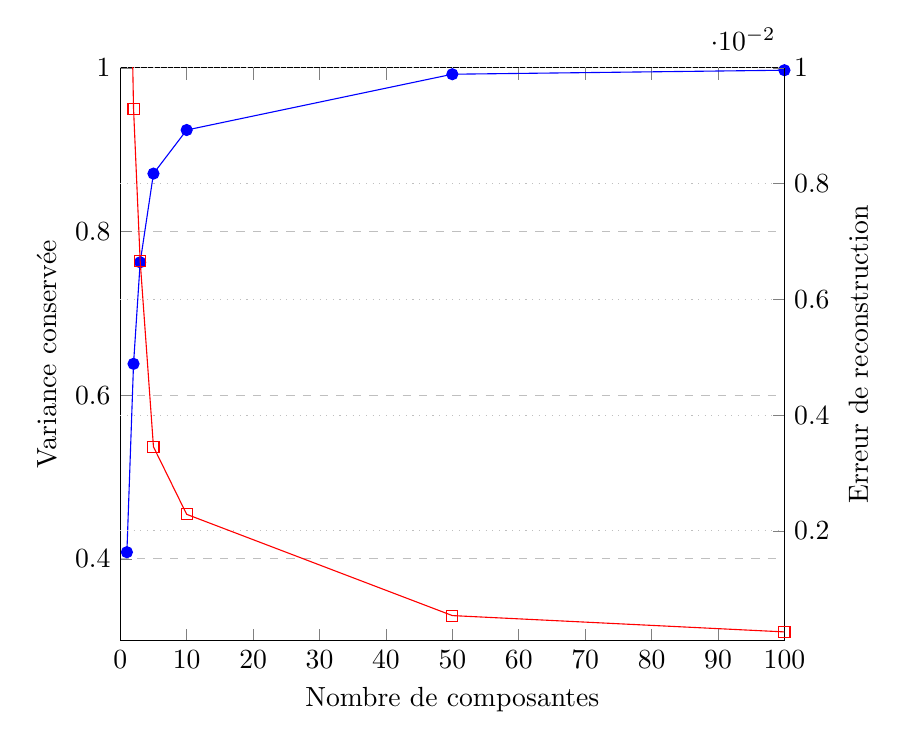
\begin{tikzpicture}
        % let both axes use the same layers
        \pgfplotsset{
            % set layers,
            xlabel=x-axis,
            legend columns=-1,
            legend style={draw=none},
            legend to name=named,
        }
        \begin{axis}[
        set layers,axis background,
        scale only axis,
        xmin=0, xmax=100,
        axis y line*=left,
        legend style={at={(0.5,-0.2)},anchor=north},
        xlabel={Nombre de composantes},
        ylabel style = {align=center},
        ylabel={Variance conservée}, % \ref{pgfplots:plot1}
        xtick={0,10,20,30,40,50,60,70,80,90,100},
        ymin=0.3, ymax=1.0,
        ytick={0.4,0.6,0.8,1.0},
        ymajorgrids=true,
        grid style=dashed,%gray
        ]
        \addplot [color=blue,mark=*]
        table{
            1 0.408233
            2 0.638416
            3 0.762465
            5 0.870857
            10 0.924131
            50 0.992305
            100 0.997201
        };
        % \addlegendentry{Erreur de reconstruction}, HINT: should be added on next axis with \addlegendimage
        \label{plot:pca_var}
        \end{axis}
        \begin{axis}[
        scale only axis,
        xmin=0, xmax=100,
        axis y line*=right,
        axis x line=none,
        ylabel style={align=center},
        ylabel={Erreur de reconstruction}, % \ref{pgfplots:plot2}
        % y dir=reverse,
        % ymode=log,
        ymin=0.0001, ymax=0.01,
        % ytick={0.0001, 0.001,0.01},
        ymajorgrids=true,
        % grid style=dashed,
        major grid style=dotted,
        axis background,
        ]
        \addlegendimage{/pgfplots/refstyle=plot:pca_var}\addlegendentry{Variance conservée}
        \addplot [color=red,mark=square]
        table{
            1 0.015433
            2 0.009297
            3 0.006661
            5 0.003452
            10 0.002285
            50 0.000535
            100 0.000253
        };
        \addlegendentry{Erreur de reconstruction},
        \label{plot:pca_mse}
        \end{axis}
        %
        \end{tikzpicture}
    \end{adjustbox}
    \\
    \ref{named}
    \caption{Qualité de la compression par \textit{ACP} en fonction du nombre de composantes.}
    \label{fig:pca_plot}
\end{figure}

\begin{figure}[hbtp]
    \centering
    \includegraphics[width=0.95\textwidth,height=\textheight,keepaspectratio]{../Chap3/Figures/visualize_PCA_pixel_space.png}
    \caption{Projection par \textit{ACP} à partir de la valeur des pixels des images. L'échelle 1-5 correspond aux niveaux de qualité évalués par les experts humains ; -1 correspond aux pièces non annotées.}
    \label{fig:ACP}
\end{figure}

La Figure \ref{fig:ACP} présente les valeurs des deux dimensions obtenues pour chaque pièce en appliquant une ACP sur la valeur des pixels bruts de l'image.
On observe une séparation intéressante des images qui ne contiennent pas de pièce, mais par exemple le bras robotique préhenseur.
En revanche, seuls deux paquets sont mis en évidences, parmi lesquels des pièces de bonnes qualité et des pièces de mauvaises qualité sont mélangées.
L'ACP réalisée sur les pixels bruts est limitée aux motifs globaux de l'image.
Il est nécessaire de réaliser un prétraitement des images pour extraire les motifs pertinents sur notre problème avant d'appliquer une ACP.
L'expertise humaine est requise pour choisir les méthodes judicieuses de prétraitement à appliquer.
Nous détaillons des approches de ce type dans la Section \ref{sec:extraction}.
L'ACP utilise ici deux uniques composantes.
Comme présenté dans les figures \ref{fig:pca_reconstruction} et \ref{fig:pca_plot}, une centaine de composantes permettent de modéliser la variance de notre jeu de données de manière satisfaisante.
Avec deux composantes, la perte de variance est de 36 \%, ce qui est important.
Il sera judicieux d'utiliser un nombre de composantes plus important, ou bien d'utiliser une méthode plus robuste tels que le \textit{t-SNE} \ref{subsubsec:tsne} ou \textit{UMAP} \ref{subsubsec:umap}.

Le calcul de la matrice de covariance $\overline{C}$ a une complexité de l'ordre de $\bigO(m^{2} \cdot N)$.
La décomposition en valeur propre a une complexité $\bigO(m^{3})$.
La complexité de l'ACP est $\bigO(m^{2} \cdot N+m^{3})$.
Soit, pour un nombre de variables constant $m \ll N$, l'ACP a une complexité linéaire $\bigO(N)$.
Ainsi, le coût de son calcul est négligeable sur les ressources informatiques modernes.
C'est une méthode très efficiente de réduction de l'information.

\subsubsection{ACP à noyau}\label{subsubsec:kpca}
L'ACP à noyau (\textit{Kernel-PCA}) réalise une ACP dans l'espace transformé par un noyau $K$ (voir la méthode de construction d'un noyau, §\ref{parag:svm}).
Elle a été proposée par \cite{scholkopf_kernel_1997, scholkopf_nonlinear_1998}.
La méthode de la transformée par noyau utilise une transformation $\varphi$ de l'espace initial des données, vers un espace où les données sont linéairement séparables.
On applique alors la méthode de l'ACP dans ce nouvel espace pour trouver les $k$ vecteurs propres $\mathbf{V}$, Équation \ref{eq:kernel_pca}.

\begin{equation} \label{eq:kernel_pca}
\begin{split}
\overline{C}_{ker}=\operatorname{cov}(\varphi(X))=\frac{1}{N} \sum_{n=1}^{N} \varphi\left(\mathbf{x}_{n}-\overline{\mathbf{x}}\right) \cdot \varphi\left(\mathbf{x}_{n}-\overline{\mathbf{x}}\right)^{\mkern-1.5mu\mathsf{T}}
\\
\lambda\left(\varphi(X) \cdot \mathbf{V}\right)=\left(\varphi(X) \cdot \overline{C}_{ker} \mathbf{V}\right)
\end{split}
\end{equation}

L'optimisation des hyper-paramètres d'une ACP à noyau (choix du noyau et de ses paramètres) peut être réalisée par recherche exhaustive d'hyper-paramètres et validation croisée.
On cherche à obtenir la transformée qui limite au maximum la corruption de l'information du jeu de données initial.
Ainsi, on cherche l'ACP qui, suite à une projection des données dans l'espace des vecteurs propres, puis à la transformée inverse dans l'espace initial, conserve les données.
La métrique utilisée est la norme Euclidienne, entre les données initiales et les données transformées puis transformées inverses, par l'ACP à noyau.

\begin{figure}[hbtp]
    \centering
    \includegraphics[width=0.95\textwidth,height=0.7\textheight,keepaspectratio]{../Chap3/Figures/KernelPCA_cv_notperf.png}
    \caption{Optimisation des paramètres d'une ACP à noyaux. Métrique : Norme $\ell_{2}$.}
    \label{fig:kernel_pca}
\end{figure}

\begin{figure}[hbtp]
    \centering
    \includegraphics[width=1\textwidth,height=0.7\textheight,keepaspectratio]{../Chap3/Figures/visualize_reconstructed_kPCA100_images.jpg}
    \caption{Compression par ACP à noyau.}
    \label{fig:kpca_reconstruction}
\end{figure}

\begin{figure}[hbtp]
    \centering
    \begin{adjustbox}{width=0.80\textwidth}
        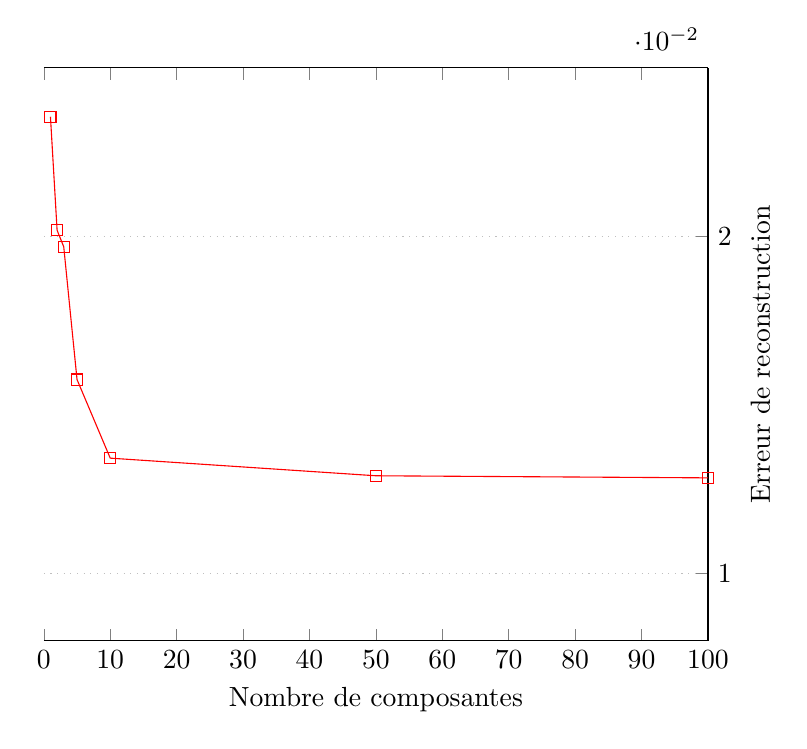
\begin{tikzpicture}
        % let both axes use the same layers
        \pgfplotsset{
            xlabel=x-axis,
            legend columns=-1,
            legend style={draw=none},
            legend to name=named,
        }
        \begin{axis}[
        scale only axis,
        xmin=0, xmax=100,
        axis y line*=right,
        xlabel={Nombre de composantes},
        ylabel style = {align=center},
        ylabel={Erreur de reconstruction}, % \ref{pgfplots:plot1}
        xtick={0,10,20,30,40,50,60,70,80,90,100},
        ymin=0.008, ymax=0.025,
        ytick={0.03,0.02,0.01},
        ymajorgrids=true,
        grid style=dotted,
        ]
        \addplot [color=red,mark=square]
        table{
            1 0.023551
            2 0.020183
            3 0.019691
            5 0.015753
           10 0.013420
           50 0.012897
          100 0.012835
        };
        \addlegendentry{Erreur de reconstruction}, %HINT: should be added on next axis with \addlegendimage
        \label{plot:kpca_mse}
        \end{axis}
        \end{tikzpicture}
    \end{adjustbox}
    \\
    \ref{named}
    \caption{Qualité de la compression par \textit{ACP à noyau} en fonction du nombre de composantes.}
    \label{fig:kpca_plot}
\end{figure}

La Figure \ref{fig:kernel_pca} présente le résultat d'une optimisation sur $k$ : le nombre de paramètres et $\gamma$ : coefficient d'un noyau \textit{RBF}. On choisira ici $k = 20$ et $\gamma = 0,02154$.

Nous obtenons des performances inférieures à l'ACP, Figure \ref{fig:kpca_reconstruction}.
La transformation par un noyau gaussien est ici inutile.
De manière générale, le traitement d'images aux textures complexes nécessite l'utilisation de modèles fortement non linéaires, ce qui n'est pas le cas du noyau gaussien.
C'est pourquoi les méthodes par réseaux de neurones non linéaire obtiennent de meilleurs résultats.
Nous les étudierons dès la section suivante, §\ref{subsubsec:vae}.

La complexité de l'ACP à noyau est $\bigO(m^{2} \cdot n^2+m^{3})$ pour un noyau linéaire et $\bigO(m^{2} \cdot n^3+m^{3})$ pour un noyau gaussien (\textit{RBF}).
Dans le cas $m \ll n$, les complexités sont quadratiques $\bigO(n^2)$ pour un noyau linéaire et cubique $\bigO(n^3)$ pour un noyau gaussien.
Lorsqu'on utilise l'ACP à noyau, on limitera le nombre de variables $m$ des échantillons.
De plus, la difficulté apparait dans le cas où le jeu de données est grand ($n > 1000$) : le coût du stockage du noyau $K$ en mémoire devient significatif.
% Linear SVM $\bigO(N   \cdot m)$
% RBF SVM    $\bigO(N^2 \cdot m)$

\subsubsection{t-SNE} \label{subsubsec:tsne}
% https://scikit-learn.org/stable/modules/clustering.html#spectral-clustering
La méthode \textit{t-SNE} (\textit{t-Distributed Stochastic Neighbor Embedding}) est proposée par \cite{maaten_visualizing_2008}. C'est une méthode de réduction de l'information itérative particulièrement adaptée à la visualisation des données dans un espace à deux ou trois dimensions.
\textit{t-SNE} est une évolution de la méthode \textit{SNE} (\textit{Stochastic Neighbor Embedding}) \cite{hinton_stochastic_2003}.
Les deux méthodes utilisent la même démarche.
Une distribution de probabilité $P$ est générée afin de modéliser la distribution des distances entre les points, pour le jeu de données initial.
Le nombre de points voisins à prendre en compte est défini par l'hyper-paramètre de \textit{perplexité}.
Une petite valeur de perplexité permet de mettre en évidence les structures locales, alors qu'une grande valeur mettra en évidence les structures globales.
La valeur de perplexité définira la variance de la distribution.
En pratique, on choisira une valeur dans $[5; 50]$.
Une distribution $Q$ est générée afin de modéliser les mêmes propriétés des données, mais dans un espace de dimensions réduites.
On cherche alors à minimiser l'écart entre les deux distributions $P$ et $Q$ afin de trouver la distribution $Q$ optimale.
Cette démarche permet de modéliser la structure non-linéaire des données.
Les paramètres de $Q$ sont ajustés par descente de gradient stochastique, afin de minimiser la divergence de Kullback-Leibler entre les deux distributions, Équation \ref{eq:D_KL}.
\textit{SNE} utilise une distribution de probabilité gaussienne, alors que \textit{t-SNE}, une distribution qui suit une loi de Student (\textit{t-distribution}).
La loi de Student est à queue-longue.
Elle tend plus lentement vers zéro qu'une distribution gaussienne.
Aussi, elle est plus adaptée à la modélisation des distances entre de petits nombres d'échantillons.
Enfin, \textit{t-SNE} propose de simplifier les calculs de l'optimisation de $Q$ en utilisant une loi de Student à un degré de liberté, qui est une loi de Cauchy, $f(t)=\frac{1}{\pi(1+t^2)}$.

Trois conséquences de la méthode limitent son utilisation à la seule visualisation de données.
La réduction de dimensions obtenue n'est pas une fonction.
Aussi, de nouveaux échantillons ne pourront pas être projetées dans l'espace réduit.
L'algorithme est stochastique et chaque exécution produit un résultat différent.
Enfin, les résultats dépendent fortement de la valeur de l'hyper-paramètre \textit{perplexité}.

\begin{figure}[htb]
    \centering
    \includegraphics[width=0.95\textwidth,height=\textheight,keepaspectratio]{../Chap3/Figures/visualize_T-SNE_pixel_space.png}
    \caption{Projection par \textit{t-SNE} à partir de la valeur des pixels des images. L'échelle 1-5 correspond aux niveaux de qualité évalués par les experts humains ; -1 correspond aux pièces non annotées.}
    \label{fig:tSNE}
\end{figure}

La Figure \ref{fig:tSNE} présente la projection obtenue par \textit{t-SNE} sur la valeur des pixels bruts de l'image de chaque pièce.
On observe une séparation en quatre paquets, dont un paquet qui contient les images "erronées" (qui ne contiennent pas de pièce).
À la différence de la projection par ACP, Figure \ref{fig:ACP}, trois paquets de différente qualité de pièces sont mis en évidences.
L'algorithme \textit{t-SNE} propose une réduction de dimensions plus pertinente que l'ACP, pour les problèmes où des motifs complexes doivent être distingués.
Cependant, appliquer cet algorithme sur les valeurs des pixels bruts limite les résultats à la séparation de motifs globaux.
Il est nécessaire de réaliser un prétraitement des images pour extraire les motifs pertinents sur notre problème.
Une approche par apprentissage supervisé et réseau de neurones de convolution est la plus pertinente.
L'apprentissage par transfert de domaine (§\ref{subsec:transfer_learning}) peut également être utilisé, comme méthode d'extraction des motifs pertinents.

Une dernière limite de cette méthode est posée par le calcul de la distance Euclidienne entre les points que l'on cherche à modéliser dans les distributions $P$ et $Q$.
La distance Euclidienne nécessite de vérifier l'hypothèse de linéarité de l'espace entre les points.
C'est une hypothèse forte qui est rarement vérifiée pour les données complexes, notamment lorsque la répartition des points n'est pas uniforme.
C'est pourquoi de nouvelles méthodes de réduction de l'information ont été proposées.
Nous nous intéresserons en particulier à la méthode \textit{UMAP} §\ref{subsubsec:umap}, qui utilise la géométrie riemannienne pour résoudre ces limites.

La complexité de l'algorithme t-SNE est de l'ordre de $\bigO(d N^2)$, avec $d$ la dimension de l'espace réduit.
\cite{maaten_accelerating_2014} propose d'accélérer l'algorithme à une complexité de $\bigO(d N \log N)$, dans le cas où $d \le 3$ en approximant le gradient par l'algorithme à arbres binaires de recherche de Barnes et Hut \cite{barnes_hierarchical_1986}.

\subsubsection{UMAP} \label{subsubsec:umap}
La méthode de réduction de l'information \textit{UMAP} est proposée par \cite{mcinnes_umap_2018, mcinnes_umap_2018a}.
Elle s'appuie sur l'apprentissage de variété (\textit{manifold learning}).
On cherche, dans l'espace de dimensions initiales, une variété (des surfaces topologiques), pour laquelle les données sont au plus proche de celle-ci.







La variété obtenue est alors une représentation des données dans un espace de dimensions réduites.
Alors que l'ACP réalise une projection dans un espace euclidien, \textit{UMAP} projette les données dans un espace riemannien.
L'espace riemannien possède les hypothèses de connexité et de complétude, ce qui limite la perte d'informations.
L'algorithme \textit{UMAP} cherche une variété $\mathbb{V}$ dans cet espace, telle que les données soient situées au plus proches de celle-ci.
Afin d'utiliser cette démarche, trois hypothèses sont faites :
\begin{itemize}
\item La distribution des données est uniforme sur la variété $\mathbb{V}$ utilisée.
\item La métrique riemannienne peut être localement approximée comme une constante.
\item L'espace riemannien utilisé est connexe.
\end{itemize}


Le théorème de Nerve affirme qu'il est possible de représenter la topologie de la variété $\mathbb{V}$ par des simplexes (c'est à dire par les éléments topologiques les plus simples possibles).
% https://ncatlab.org/nlab/show/nerve+theorem
% K. Borsuk, On the imbedding of systems of compacta in simplicial complexes , Fund. Math 35, (1948) 217-234
% J. Leray. Sur la forme des espaces topologiques et sur les points fixes des représentations. J. Math. Pures Appl. 24:95–167, 1945
Dans ce cas, $\mathbb{V}$ et sa représentation en simplexes sont équivalentes.
Il est alors possible de modéliser ces simplexes par une distribution combinatoire $P$, en appliquant la logique floue (topologie-floue).
Nous invitons le lecteur qui souhaite approfondir la méthode, à consulter le papier original des auteurs de l'algorithme \cite{mcinnes_umap_2018}.
Par la suite, représenter les données dans un espace de petites dimensions, revient à trouver la variété de petites dimensions qui possède la distribution $Q$ la plus similaire possible avec la distribution $P$ de la variété des données initiales.
Cela revient à trouver la distribution $Q$ telle que l'entropie croisée entre les deux distributions $P$ et $Q$ soit minimale.
Cette démarche est similaire à la minimisation de la divergence de Kullback-Leibler de \textit{t-SNE} §\ref{subsubsec:tsne} qui met en évidence la structure locale des données, mais elle permet également de préserver la structure globale.

% -> I am using the UMAP for Dimensionality Reduction. It's implementation really bods well with my data. I have a question regarding the feature importance. Suppose, after the dimensionality reduction, the UMAP separates out the labels clearly and creates the 3 subgroups containing all labels. Can I somehow get the list of features corresponding to each group? Which features were more relevant to which group?
% -> One option that I have seen done is to build a classifier based on the clusters and then use SHAP or LIME to get interpretations of what separates the clusters.

\begin{figure}[hbtp]
    \centering
    \includegraphics[width=\textwidth,height=\textheight,keepaspectratio]{../Chap3/Figures/visualize_UMAP_pixel_space.png}
    \caption{Représentation par \textit{UMAP} à partir de la valeur des pixels des images. L'échelle 1-5 correspond aux niveaux de qualité évalués par les experts humains ; -1 correspond aux pièces non annotées.}
    \label{fig:umap}
\end{figure}

La Figure \ref{fig:umap} présente la représentation en deux dimensions obtenues en appliquant \textit{UMAP} sur la valeur des pixels brutes de l'image.
En comparaison de \textit{t-SNE}, \textit{UMAP} permet de mettre en évidence la structure globale des données dans les deux dimensions, tout en conservant la structure locale des paquets d'échantillons.
Les images qui ne contiennent pas de pièces sont séparées, ainsi que le paquet de pièces annotées d'un niveau de qualité 0 (mauvais).
De plus, le niveau de qualité 1 est séparé.
Les niveaux 2 à 5 sont représentés dans deux paquets distincts.
Il apparait un paquet de pièces de très bonne qualité (niveau 5).
Ce paquet contient quelques pièces des niveaux 3 et 4 ; aussi cela indique que l'annotation humaine n'est pas robuste lorsque l'on approche de la qualité maximale.
En comparaison des résultats obtenus avec un réseau de triplets, Figure \ref{fig:triplet_result}, cette méthode présente une séparation des paquets identiques, mais sans annotation humaine et avec un coût de calcul plus de cent fois moindre.
L'approche topologique permet d'améliorer les performances et la méthode \textit{UMAP} montre son intérêt dans le cadre d'une approche non-supervisée de suggestion d'annotation à l'expert humain.

Afin de trouver le graphe de la représentation en petites dimensions, \textit{UMAP} utilise l'algorithme (\textit{Nearest-Neighbor-Descent}) d'optimisation de graphes proposé par \cite{dong_efficient_2011}.
Les auteurs évaluent empiriquement la complexité de leur méthode de l'ordre de $\bigO(N^{1.14})$.
Aussi, la complexité de la méthode \textit{UMAP} est limitée par cet algorithme.
Elle est de l'ordre de $\bigO(N \log N)$.

% ivis: structure preserving dimensionality reduction
% https://bering-ivis.readthedocs.io/en/latest/

\subsubsection{Auto-encodeurs variationnels} \label{subsubsec:vae}.
Un auto-encodeur cherche à reproduire la donnée entrée, avec le minimum de paramètres (ou Degrés De Liberté).
Aucune annotation des données n'est requise.
C'est une méthode qui permet d'apprendre la représentation des données dans un espace de dimensions réduites (aussi appelé \textit{feature learning} ou \textit{representation learning}).
En 1987, \cite{lecun_modeles_1987, gallinari_memoires_1987} proposent un réseau auto-encodeur utilisant des réseaux de neurones, afin de supprimer le bruit d'images.
Dans leurs travaux, ils étudient la capacité du réseau à mémoriser les caractéristiques des images initiales, en fonction de son architecture.
En parallèle, \cite{ballard_modular_1987} propose un auto-encodeur (appelé ici \textit{systèmes auto-associatifs}) à trois couches.
Dans ces travaux, les poids des neurones sont ajustés par rétro-propagation du gradient, récemment proposée.

Un auto-encodeur se compose de deux parties : un encodeur $z = f(x)$ qui compresse l'information initiale dans un espace de dimensions réduites (appelé \textit{espace latent}) et un décodeur $\hat x = g(z)$ qui reconstruit ensuite une approximation de $x$ à partir de $z$.
$f$ et $g$ sont généralement des réseaux de convolutions profonds, dont les poids respectifs sont $\mathbf{W}_f$ et $\mathbf{W}_g$.
La Figure \ref{fig:autoencoder_architecture} présente l'architecture d'un auto-encodeur qui utilise des réseaux de convolutions pour ces fonctions.

\begin{figure}[hbtp]
    \centering
    \includegraphics[width=\textwidth,height=\textheight,keepaspectratio]{../Chap3/Figures/autoencoder_architecture.pdf}
    \caption{Architecture d'un auto-encodeur.}
    \label{fig:autoencoder_architecture}
\end{figure}

Afin de mesurer la similitude telle que $x \simeq \hat x$, la fonction de coût à minimiser lors de l'apprentissage du modèle est souvent l'erreur quadratique entre $x$ et $\hat x$, Équation \ref{eq:autoencoder}.

\begin{equation} \label{eq:autoencoder}
\min _{\mathbf{W}_{f}, \mathbf{W}_{g}} \mathcal{L}_{g\acute{e}n\acute{e}ration}\left(x, \hat{x}\right) = \min _{\mathbf{W}_{f}, \mathbf{W}_{g}} \left\|x-g\left(f\left(x, \mathbf{W}_{f}\right), \mathbf{W}_{g}\right)\right\|_{2}^{2}
\end{equation}

Enfin, une contrainte indispensable est appliquée à la dimension de $z$, qui doit être très petite devant la dimension de $x$.
Ainsi, seules les propriétés les plus importantes des données sont prises en compte.
Un cas particulier apparait si le décodeur $g$ est une application linéaire et si la fonction de coût est l'erreur quadratique : alors les valeurs de $z$ sont équivalentes aux valeurs propres d'une Analyse en Composante Principale \cite{bourlard_autoassociation_1988}.

La Figure \ref{fig:autoencoder} présente une image entrée et sa reconstruction après le passage dans un auto-encodeur dont $z$ a une dimension de 128 valeurs.
On observe la perte d'information visuelle : la marque de l'éjecteur a, par exemple, disparu.
En revanche, les défauts d'aspect qui nous intéressent sont reproduits.
Le taux de compression est ici de 120 : $124 \times 124$ pixels $\rightarrow 128$ valeurs.
À la différence de la compression par ACP, Figure \ref{fig:pca_reconstruction}, la reconstruction ne possède pas d'artefacts.
En revanche, le coût de calcul de cette méthode est beaucoup plus grand que pour une ACP.
Il est nécessaire de disposer d'une accélération des calculs massivement parallèle, par exemple sur processeur graphique, pour pouvoir construire un modèle à partir d'un grand nombre d'échantillons.

\begin{figure}[hbtp]
    \centering
    \includegraphics[width=0.75\textwidth,height=\textheight,keepaspectratio]{../Chap3/Figures/visualize_reconstructed_variations.png}
    \caption{Reconstruction d'une image par un auto-encodeur.}
    \label{fig:autoencoder}
\end{figure}

La Figure \ref{fig:tSNE_ae} présente les valeurs des 128 dimensions de $z$ projetées par l'algorithme \textit{t-SNE}, présenté dans la Section \ref{subsubsec:tsne}.
Les différentes classes exprimées dans l'espace latent $z$ sont mieux séparées que dans la Figure \ref{fig:tSNE} qui utilisait les données brutes : l'ensemble des valeurs des pixels.
On observe également que l'évaluation des cinq classes de qualité, évaluées par les experts humains, est respectée.
Les pièces non annotées sont positionnées dans les bonnes classes.
Enfin, il est intéressant d'observer qu'un paquet correspondant à une erreur de mesure, comme par exemple l'absence de pièces et la capture du bras robotique préhenseur est mis en évidence.

\begin{figure}[hbtp]
    \centering
    \includegraphics[width=0.95\textwidth,height=\textheight,keepaspectratio]{../Chap3/Figures/visualize_T-SNE_latent_space.png}
    \caption{Projection par \textit{t-SNE} à partir des valeurs de l'espace latent $z$ d'un \textit{VAE}. L'échelle 1-5 correspond aux niveaux de qualité évalués par les experts humains ; -1 correspond aux pièces non annotées.}
    \label{fig:tSNE_ae}
\end{figure}

% Séparabilité des classes
% Neighborhood Hit score
% Fernando Vieira Paulovich, Luis Gustavo Nonato, Rosane Minghim, and Haim Levkowitz. Least square projection: A fast high-precision multidimensional projection technique and its application to document mapping. IEEE Trans. Vis. Comput. Graph., 14(3):564–575, 2008
% http://cedric.cnam.fr/vertigo/Cours/ml2/tpDeepLearning4.html#exercice-3-separabilite-des-classes-et-representations-internes-des-reseaux-de-neurones

Un auto-encodeur modélise une application (encodeur $x \rightarrow z$) et l'application inverse (générateur $z \leadsto \hat x$).
Cependant, il est difficile d'interpoler les valeurs de $z$ afin de générer des $\hat x$, car l'espace $z$ n'a pas de contrainte de continuité ; aussi $z$ est généralement discontinue.
Récemment, l'auto-encodeur variationnel (\textit{Variational Auto-Encoder}) est proposé par \cite{kingma_autoencoding_2013, rezende_stochastic_2014}.
Il utilise une méthode d'inférence variationnelle.
À la différence d'un auto-encodeur, un VAE modélise le générateur $g$ sous la forme d'une distribution de probabilité $p(x | z)$ sur les données.
De même, l'encodeur $f$ sera une distribution $q(z | x)$.
Un a priori fort sur la distribution $q$ est introduit : on cherche généralement $q(z | x)$ qui soit proche d'une gaussienne centrée $\mathcal{N}(\mu=0,\sigma=1)$.
Ainsi, $q$ sera continue.
Cette condition revient à minimiser la divergence de Kullback-Leibler entre la distribution de l'encodeur $q(z | x)$ et la distribution du générateur $p(z | x)$.
L'auto-encodeur variationnel nécessite une fonction de coût composite, Équation \ref{eq:vae}.

\begin{equation} \label{eq:vae}
\begin{split}
\mathcal{L}_{VAE} = \mathcal{L}_{g\acute{e}n\acute{e}ration} + \mathcal{L}_{latent}
\\
\text{avec } \mathcal{L}_{latent}\left(\hat{y}, y\right) = Divergence_{K L}\left(p(z | x) \| N(\mu=0 ; \sigma=1)\right)
\end{split}
\end{equation}

\begin{figure}[hbtp]
    \centering
    \includegraphics[width=\textwidth,height=\textheight,keepaspectratio]{../Chap3/Figures/vae_from_Doersh2016.pdf}
    \caption{Graphe d'un auto-encodeur variationnel, inspiré de \cite{doersch_tutorial_2016}.}
    \label{fig:vae}
\end{figure}

Lors de l'apprentissage, les distributions $p$ et $q$ sont modélisées par des réseaux de neurones.
Les sorties du générateur seront les paramètres de la distribution : la moyenne et l'écart-type, tels que $q(z | x) = \mathcal{N}\left(z ; \vec{\mu}(x), \operatorname{diag}(\vec{\sigma}(x))^{2}\right)$.
La Figure \ref{fig:vae}, inspirée de \cite{doersch_tutorial_2016}, représente le graphe de calcul de ce modèle.
Il devient possible de générer de nouvelles sorties à partir de la distribution $p(z)$, en tirant les valeurs de $z$ à partir de la distribution $\mathcal{N}(\mu=0,\sigma=1)$.
Ces nouvelles sorties ne sont pas nécessairement similaires aux données d'apprentissages de $x$.
Ainsi, l'auto-encodeur variationnel généralise l'auto-encodeur et le rend \textit{génératif}.

\begin{figure}[hbtp]
    \centering
    \includegraphics[width=\textwidth,height=\textheight,keepaspectratio]{../Chap3/Figures/visualize_interpolations_latent.jpg}
    \caption{Génération d'images à partir de la distribution modélisant l'espace latent d'un auto-encodeur variationnel.}
    \label{fig:vae_sampling}
\end{figure}

La Figure \ref{fig:vae_sampling} montre des images générées à partir de tirages aléatoires sur la distribution $P$ de l'espace latent $z$.
On observe la diversité des défauts modélisés dans $z$, mais également le réalisme limité que produit le générateur d'un VAE.
Cela est dû à la compression élevée et au petit jeu de données dont nous disposons ce qui entraine du bruit.
Il est intéressant d'observer des artefacts de couleur bleu, qui correspondent à la présence d'images dans le jeu de données où il n'y pas de pièce, mais où le bras robotique de couleur bleue est présent.
Le bras robotique est néanmoins très peu présent dans $z$ en comparaison des pièces : le VAE est robuste.

Les réseaux génératifs permettent de palier de manière intéressante au manque de variétés des échantillons dans les petits jeux de données.
Cependant, les images générées sont souvent floues, ce qui est souvent dû à la fonction de coût, l'erreur moyenne entre $x$ et $\hat x$, utilisée lors de l'apprentissage.
En effet, l'erreur moyenne ne permet pas la prise en compte dans $z$ des motifs complexes qui sont peu présents dans le jeu de données.
Dernièrement, \cite{kingma_introduction_2019} propose une synthèse exhaustive des solutions à cette problématique : construire des modèles plus profonds, ajouter des contraintes plus pertinentes dans la fonction de coût, comme par exemple des tâches de classification auxiliaires, et mettre à jour de manière plus judicieuse les poids lors de l'apprentissage du modèle.
Un autre type de modèle génératif propose également d'améliorer le réalisme des images générées.
L'apprentissage n'est pas réalisé sur l'erreur entre $x$ et $\hat x$, mais de manière indirecte à partir de la valeur retournée par un second modèle.
Ce principe permet d'améliorer le réalisme en prenant en compte des motifs complexes lors de la reconstruction.
Il s'agit des modèles antagonistes génératifs que nous détaillons dans la Section \ref{subsubsec:GAN}.

L'apprentissage d'un modèle VAE est réalisé par descente de gradient stochastique.
Les poids du modèle sont ajustés sur un sous-ensemble du jeu de données de taille $B$ échantillons (appelé mini-batch), pendant $T$ itérations.
La complexité de l'apprentissage est de l'ordre de $\bigO(T B^2 D + T B^2 d)$, avec $T$ le nombre d'itérations, $B$ le nombre d'échantillons dans un mini-batch, $D$ la dimension d'un échantillon et $d$ la dimension de l'espace latent.
De plus, la quantité de mémoire de travail nécessaire au stockage des mini-batch est de l'ordre de  $\bigO(B^2 D)$.
Ces coûts de calcul sont importants.
Dans nos expériences, c'est la quantité de mémoire de travail sur le processeur graphique dont nous disposons (11 Giga octets) qui conditionne le nombre d'échantillons par mini-batch (ici, $B=64$ et $D=128^2$), d'où la complexité des calculs ($T=100$, $B=64^2$, $D=128^2$). Nous obtenons une complexité de l'ordre de 7 Milliards d'opérations et une occupation mémoire de l'ordre de 10 Giga octets.
La durée de l'apprentissage de notre modèle VAE est d'une heure sur un processeur graphique dédié (\textit{NVIDIA GTX 1080 Ti}).
Avec les ressources informatiques actuelles, une mise à jour journalière de ce modèle peut être envisagée, lors de son utilisation au sein d'un procédé industriel.

% Great ressources on AE & VAE:
% https://www.deeplearningbook.org/contents/generative_models.html
% https://ermongroup.github.io/cs228-notes/extras/vae/
% http://anotherdatum.com/vae.html
% http://anotherdatum.com/vae2.html
% http://anotherdatum.com/vae-moe.html
% https://arxiv.org/abs/1606.05908 Tutorial on Variational Autoencoders
% Diederik P. Kingma PhD thesis: Variational inference & deep learning: A new synthesis
% https://bjlkeng.github.io/posts/variational-autoencoders/
% https://bjlkeng.github.io/posts/a-variational-autoencoder-on-the-svnh-dataset/
% http://www.cs.toronto.edu/~urtasun/courses/CSC2541_Winter17/Deep_generative_models.pdf
% Adversarial Autoencoders arXiv:1511.05644
% Bayesian NN http://anotherdatum.com/bnn.html

% \cite{kingma_semisupervised_2014}
% https://bjlkeng.github.io/posts/semi-supervised-learning-with-variational-autoencoders/
% https://github.com/bjlkeng/sandbox/tree/master/notebooks/vae-semi_supervised_learning
% Auxiliary Deep Generative Models https://arxiv.org/abs/1602.05473
% One-shot: Danilo Jimenez Rezende, Shakir Mohamed, Ivo Danihelka, Karol Gregor, and Daan Wierstra. One-shot generalization in deep generative models. arXiv preprint arXiv:1603.05106, 2016b.

% ELBO surgery https://rachitsingh.com/elbo_surgery/
% Fixing a broken ELBO https://lyusungwon.github.io/generative-models/2018/06/29/fbe.html

% https://arxiv.org/abs/1906.00446, Generating Diverse High-Fidelity Images with VQ-VAE-2, June 2019

% Nous proposons l'architecture suivante : split_coef doit être un diviseur de 1920 et un carré parfait : [1, 4, 16, 32, 64]

\subsubsection{Réseaux antagonistes génératifs} \label{subsubsec:GAN}
Proposés par \cite{goodfellow_generative_2014}, les réseaux antagonistes génératifs (\textit{Generative Adversarial Networks}) permettent de raffiner le modèle de l'espace latent.
En comparaison avec les auto-encodeurs, les images issues du générateur sont plus proches des images originales.
Les \textit{GAN} s'appuient sur une association de deux modèles qui sont entrainés en concurrence : un générateur $g$ génère $\hat x = g(z)$ et un classifieur $d$ (appelé \textit{discriminateur}) calcule la probabilité $p$ que $\hat x$ appartienne au jeu de donnée réel, $p = d(x)$.
L'objectif du générateur est de générer $\hat x$ tel que $\hat x \simeq x$, tandis que l'objectif du discriminateur est de distinguer les $\hat x$ générés par le générateur, des $x$ réels, issues du jeu de données initial.
La phase d'apprentissage de ce modèle est similaire à un duel de la théorie du jeu où le générateur et son adversaire le discriminateur s'affrontent.
Les deux modèles sont entrainés en parallèle afin d'apprendre les poids $w_g$ et $w_d$ qui maximiseront leurs performances.
Un équilibre de Nash \cite{nash_equilibrium_1950, nash_noncooperative_1951} est théoriquement atteint lorsque le générateur produit des $\hat x$ qui ne peuvent plus être distingués des $x$ par le discriminateur.
Trouver le générateur $g$ optimal revient à résoudre le problème d'optimisation de l'Équation \ref{eq:GAN} pour toute donnée d'entrée $x$.
Cependant, comme le problème d'optimisation cherche à minimiser un terme et minimiser un autre terme, la solution optimale est difficile à obtenir lors de l'ajustement des poids par descente de gradients stochastique car de nombreux optimums locaux (optimum pour un seul des membres) existent \cite{goodfellow_generative_2014}.

\begin{equation} \label{eq:GAN}
g_{optimal}  = \min _{g} \max _{d} = \mathbb{E}_{\mathbf{x} \sim p_{\text { réelle }}} \log d(\boldsymbol{x})+\mathbb{E}_{\boldsymbol{x} \sim p_{\text { générée }}} \log (1-d(\boldsymbol{x}))
\end{equation}

Le modèle \textit{GAN} fait partie des nombreux modèles proposés depuis les années 1990, qui s'appuient sur un apprentissage non-supervisé par affrontement de deux modèles qui s'opposent dans un jeu de minimisation-maximisation.
\cite{schmidhuber_unsupervised_2019} propose une revue des travaux fondateurs sur le sujet.
Le dynamisme actuel de la littérature sur les modèles de type \textit{GAN}, ainsi que la disponibilité des implémentations ouvertes par leurs auteurs, nous a permis d'évaluer ces modèles sur notre problématique.
De nombreux modèles utilisant des idées proches restent à évaluer.
Ils pourraient permettre d'obtenir de meilleures performances sur notre problématique d'analyse de la qualité.

À la suite de la proposition originale, \cite{radford_unsupervised_2015} propose des règles pour adapter les \textit{GAN} à la reconstruction d'images : remplacer les couches de moyenne (\textit{pooling}, §\ref{parag:pooling}) par des convolutions de noyaux $1 \times 1$, utiliser la normalisation de lot \ref{parag:batchnorm}, ne pas utiliser de couches pleinement connectées, utiliser l'activation \textit{ReLU} \ref{subsubsec:activation} pour le générateur sauf pour la dernière couche \textit{tanh}, utiliser \textit{LeakyReLU} pour le discriminateur et enfin des règles de construction de l'architecture du réseau qu'ils nomment \textit{DCGAN}.
Ce travail évalue ces règles avec comme objectif d'encoder des jeux de données d'images complexes dans un espace latent de dimensions 100.
Enfin, le travail montre l'intérêt des \textit{GAN} pour réaliser une classification d'images de manière non-supervisée (pas d'annotation des données d'apprentissage).
Il s'agit d'utiliser le générateur comme fonction d'extraction des valeurs pertinentes d'une image (espace latent), puis ensuite d'utiliser un classifieur \textit{SVM} \ref{parag:svm} sur ces dimensions de l'espace latent.
Les performances sont légèrement inférieures à celles obtenues par une approche supervisée, ce qui montre l'intérêt de la méthode puisqu'il n'a pas été nécessaire d'annoter les données pour obtenir ce résultat.
Le \textit{GAN}, puisqu'il est entrainé pour reconstruire une image à partir des dimensions réduites de l'espace latent, permet également d'extraire l'information pertinente des images.
Cette approche est particulièrement intéressante et nous chercherons à l'utiliser afin de répondre aux problèmes industriels où les jeux de données sont petits.

Par la suite, \cite{salimans_improved_2016} complète les règles du modèle \textit{DCGAN} et \cite{odena_semisupervised_2016, salimans_improved_2016} proposent en parallèle de réaliser l'apprentissage de manière semi-supervisée.
L'objectif est de créer un discriminateur qui soit également capable de répondre au problème de classification d'un jeu de données annotées.
Il s'agit d'introduire dans le jeu de données annotées une nouvelle classe "image générée".
Pour un jeu de données comportant $K$ classes, on obtient un jeu de données de $K+1$ classes.
On utilise alors le générateur pour produire les images correspondant à cette nouvelle classe $K+1$.
Cette démarche est alors introduite dans la fonction de coût du discriminateur, Équation \ref{eq:GAN_semisup}.
Ainsi, on obtient un discriminateur qui répond au problème de classification supervisée, tout en étant capable de distinguer les images générées par le générateur.
L'intérêt est double : augmentation artificielle du jeu de données et robustesse aux échantillons adversaires (les "fausses" images générées).
% arXiv:1804.09170v4 Realistic Evaluation of Deep Semi-Supervised Learning Algorithms 

\begin{equation} \label{eq:GAN_semisup}
g_{optimal}  = \min _{g} \max _{d} = \mathbb{E}_{\mathbf{x} \sim p_{\text { réelle }}} \log d(\boldsymbol{x})+\mathbb{E}_{\boldsymbol{x} \sim p_{\text { générée }}} \log (1-d(\boldsymbol{x}))
\end{equation}

Par la suite, des améliorations importantes sont apportées à la méthode. \cite{arjovsky_wasserstein_2017} propose de modifier la fonction de coût du discriminateur qui évalue la qualité de la reconstruction en utilisant la distance de Wasserstein.
\cite{gulrajani_improved_2017}, ainsi que la normalisation spectrale \cite{miyato_spectral_2018}.

L'ensemble de la littérature évalue les performances de ces modèles sur la base de données \textit{ImageNet}.
Dans notre cas, le nombre de classes est faible (deux classes : qualité bonne ou qualité mauvaise, voir au maximum une dizaine de classes par typologie de défauts).
C'est pourquoi un réseau génératif simple est capable de réaliser une synthèse fidèle des images.
En revanche, sur une base de données qui comporte une grande variété de classes, comme \textit{ImageNet}, il apparait que les modèles génératifs ne permettent pas de modéliser les associations entre des éléments géométriques qui doivent nécessairement être présents dans les images d'une classe.
Un exemple est celui de la représentation d'un chien, auquel la texture de pelage est bien appliquée par le modèle \textit{GAN}, mais qui ne possède pas quatre pattes attachées au corps.
%https://lilianweng.github.io/lil-log/2018/06/24/attention-attention.html
Cette limite provient de l'opérateur de convolution qui est une opération locale spatialement contrainte.
Par exemple, l'opérateur de convolution ne peut pas associer la valeur du pixel située en haut à gauche, avec celle en bas à droite.
De plus, lors de l'ajustement des poids par rétro-propagation du gradient, il n'y a pas de relation spatiale entre la valeur en sortie de convolution et les valeurs en entrées.
Cette problématique est critique dans le domaine du traitement de textes et la traduction (\textit{Natural Language Processing}) : la sémantique d'une phrase dépend de la position des mots dans la phrase.
% Also, Neural Turing Machines, by Alex Graves, Greg Wayne, Ivo Danihelka, Oct 2014, https://arxiv.org/abs/1410.5401
C'est pourquoi le mécanisme d'\textit{attention} a été proposé par \cite{bahdanau_neural_2014} pour la traduction de texte, puis étendu à l'analyse d'images par des convolutions par \cite{xu_show_2015}.
Par la suite, \cite{vaswani_attention_2017} propose l'architecture de couche \textit{transformer}, qui généralise la méthode en éliminant l'usage de réseaux récurrents.
% http://www.peterbloem.nl/blog/transformers
Ils montrent qu'un réseau constitué uniquement de couches d'\textit{attention} permet d'atteindre les performances de l'état de l'art en traduction de texte.
L'\textit{attention} est depuis utilisée dans toutes les méthodes de l'état de l'art en traduction automatique.
Une couche d'\textit{attention} pondère la valeur d'entrée par une distribution de probabilité, dont les paramètres sont appris, et qui dépend de la position spatiale de la valeur entrée.
Cette démarche est similaire aux portes d'activations des réseaux \textit{LSTM}, ainsi qu'à l'architecture des \textit{Highway Networks}, §\ref{subsubsec:ResNet}, §\ref{eq:highway}.

Dernièrement, \cite{zhang_selfattention_2018} propose le modèle \textit{SAGAN} (\textit{Self-Attention Generative Adversarial Networks}) qui associe l'utilisation de multiples méthodes et introduit l'utilisation du mécanisme d'\textit{attention}.
Il s'agit pour la couche d'\textit{attention} de modéliser une relation de dépendance pour un pixel, entre tous les autres pixels.
Il n'y a ainsi plus de restriction spatiale aux convolutions.

% https://towardsdatascience.com/not-just-another-gan-paper-sagan-96e649f01a6b
% https://xlnwel.github.io/blog/deep%20learning/SAGAN/
% Spatial transformer Jaderberg et al., 15, is not rly transformer/attention

\begin{figure}[hbtp]
    \centering
    \includegraphics[width=\textwidth,height=\textheight,keepaspectratio]{../Chap3/Figures/SAGAN_fake_50000.jpg}
    \caption{Génération d'images à partir de la distribution modélisant l'espace latent du générateur d'un \textit{GAN}.}
    \label{fig:gan_sampling}
\end{figure}

La Figure \ref{fig:gan_sampling} montre des images générées à partir de tirages aléatoires dans l'espace latent du générateur d'un modèle \textit{SAGAN}.
On observe le meilleur réalisme des images obtenues, en comparaison des résultats donnés par un VAE \ref{fig:vae_sampling}.
La diversité des défauts est bien représentée. De plus, il est intéressant de remarquer que malgré le très faible nombre d'images représentant un bras robotique dans le jeu de données initial (1 erreur de capture pour 100 images), ces derniers sont représentés avec beaucoup de réalisme dans l'espace latent du générateur.
Un modèle GAN est peu robuste.
Il est sensible aux échantillons extrêmes d'un jeu de données.
Dans notre cas, cela peut être un avantage pour modéliser des défauts qui n'apparaissent pas souvent ; mais cela demande également une rigueur dans la construction du jeu de données, pour ne pas introduire d'images erronées, comme ici le bras robotique.

De même que pour le modèle \textit{VAE}, §\ref{subsubsec:vae}, la complexité de l'apprentissage d'un \textit{GAN} est très importante.
L'apprentissage du modèle est réalisé par descente de gradients stochastiques.
Les poids du modèle sont ajustés sur un sous-ensemble du jeu de données de taille $B$ échantillons (appelé mini-batch), pendant $T$ itérations.
La complexité de l'apprentissage est de l'ordre de $\bigO(T B^2 D + T B^2 d)$, avec $T$ le nombre d'itérations, $B$ le nombre d'échantillons dans un mini-batch, $D$ la dimension d'un échantillon et $d$ la dimension de l'espace latent.
Nous sommes limités par la capacité de mémoire de travail de notre processeur graphique à $B=64$ et $D=128^2$, d'où la complexité des calculs ($T=5000$, $B=64^2$, $D=128^2$). Nous obtenons une complexité de l'ordre de 350 Milliard d'opérations.
La durée de l'apprentissage de notre modèle GAN est de 10 heures sur un processeur graphique dédié (\textit{NVIDIA GTX 1080 Ti}).
Avec les ressources informatiques actuelles, seule une mise à jour hebdomadaire de ce modèle peut être envisagée.
Malgré le réalisme de la méthode, il est nécessaire de disposer d'importantes ressources de calculs (au minimum 10 processeurs graphiques comme le notre) pour mettre à jour le modèle à une fréquence journalière.

% TODO: BIGGAN \textit{BIGGAN} \cite{brock_large_2018}
% https://towardsdatascience.com/gan-ways-to-improve-gan-performance-acf37f9f59b
% https://medium.com/@jonathan_hui/gan-rsgan-ragan-a-new-generation-of-cost-function-84c5374d3c6e

% http://ganocracy.csail.mit.edu/tutorial/more_resources.html
% Lipschitz Generative Adversarial Nets https://arxiv.org/abs/1902.05687

% TODO:
% Modal loss instead of MSE !!!
% Late merging 4 VAE on 4 cameras, losses on each images reconstruction
% Compare UMAP reduction with VAE reduction

% Tesla ICML Multitask/Multiinstance learning. Which part of the model to train? Supsampling?

% Long Short Term Memory
% Jurgen Schmidhuber (1997).
% Discovering Neural Nets with Low Kolmogorov Complexity and High
% Generalization Capability.
% Neural Network
%
% Deep Belief Networks
% Geoff. Hinton and S. Osindero and Yeh Weh Teh (2006).
% A fast learning algorithm for deep belief nets.
% Neural Computation.

% Vapnik 2019: Rethinking statistical learning theory: learning using statistical invariants
% https://doi.org/10.1007/s10994-018-5742-0
% This paper introduces a new learning paradigm, called Learning Using Statistical Invariants (LUSI)
%page 39: 16 The idea of two-stage learning is also realized in deep neural networks (DNN), where, at the first stage (using “deep architecture”), an appropriate network is constructed and then, at the second stage, using standard for NN training procedures, the solution is obtained. DNN, however, cannot guarantee either that the constructed network contains a good approximation to the desired function or that it can find the best solution for the given network.
% Le choix des hyperparamètres est équivalent à l'introduction de prédicat.
% Il s'agit de trouver, de manière efficiente, le ou les quelques prédicats nécessaires et suffisants, à la construction du modèle optimal.

\section{Optimisation automatique des hyper-paramètres d'un modèle} \label{section:auto_ml}
Les algorithmes présentés dans la section précédente possèdent plusieurs dizaines d'hyper-paramètres.
Leur ajustement est souvent crucial pour obtenir des performances satisfaisantes.
On parle d'optimisation des hyper-paramètres : on cherche à optimiser la performance du modèle pour la tâche à effectuer.
Il est également nécessaire de sélectionner les bonnes méthodes de préparation des données.
Le Tableau \ref{tab:cnn_hyperparameters} recense, par exemple, les hyper-paramètres des modèles à réseaux de neurones de convolutions profonds.
Des méthodes d'optimisation automatique de ces hyper-paramètres ont été proposées.
Cette optimisation est souvent appelée \textit{AutoML} (\textit{Automated Machine Learning}).
Dans le cas des réseaux de neurones profonds, l'architecture du réseau est également importante.
Elle doit être considérée comme de nombreux hyper-paramètres.
Le nombre de paramètres devient alors très grand et les algorithmes d'optimisation traditionnels deviennent limités ; la méta-descente de gradients et les algorithmes évolutionnistes deviennent plus adaptés §\ref{subsec:nas}.
Cette section propose de parcourir les méthodes les plus avancées et de discuter de leurs applications sur notre problématique de modélisation du contrôle de la qualité.

L'ensemble des expériences d'optimisation de modèles réalisées dans ces travaux ont utilisé la librairie \textit{Sacred} \cite{greff_sacred_2017}, afin de conserver un historique des hyper-paramètres et des performances associés.
Certaines de ces optimisations peuvent prendre plusieurs jours, c'est pourquoi il est nécessaire de sauvegarder l'évolution des performances pour éviter toute perte de ressources temporelles en cas d'erreur.
\textit{Sacred} permet également de rendre compte de la progression des optimisations et de surveiller toute erreur.

\subsection{Optimisation par recherche aléatoire} \label{subsec:random_search}
Afin de réaliser l'optimisation, il s'agit d'évaluer la performance de la méthode sur la plage de valeurs de chacun des hyper-paramètres.
Il est possible d'évaluer l'ensemble de la plage de valeurs de manière exhaustive, par une grille d'essais régulière, ce qui est coûteux sur le plan du calcul.
Une démarche plus économique est le tirage aléatoire sur la plage de valeurs, proposé par \cite{bergstra_random_2012}.

\begin{figure}[hbtp]
    \centering
    \includegraphics[width=0.80\textwidth,height=\textheight,keepaspectratio]{../Chap3/Figures/bergstra_RandomSearch2002.png}
    \caption{Optimisation d'une fonction à deux variables avec neuf essais. Figure reproduite de \cite{bergstra_random_2012}.}
    \label{fig:random_search}
\end{figure}

La Figure \ref{fig:random_search} présente un tirage de 9 essais pour trouver le maximum d'une fonction à deux dimensions.
Dans le cas de la recherche exhaustive, seuls trois essais permettent d'étudier la dimension horizontale.
Dans la recherche aléatoire, les 9 essais permettent d'étudier la dimension horizontale, ce qui est plus efficient.
Cette limite de la recherche exhaustive est d'autant plus importante que le nombre de dimensions étudiées est grand.
Des méthodes plus évoluées qui ont été proposées.

% https://slideslive.com/38917537/towards-semiautomated-machine-learning
% https://joaquinvanschoren.github.io/ML-course/slides_pdf/AutoML%20-%20Introduction.pdf

En 2011, \cite{bergstra_algorithms_2011} réalise un état de l'art des méthodes d'optimisations d'hyper-paramètres, pour les modèles à réseaux de neurones profonds.
Ce travail montre l'intérêt de l'optimisation itérative, basée sur le critère de la prédiction de l'amélioration de performance du modèle (\textit{Expected Improvement}, proposée par \cite{jones_taxonomy_2001}).
L'étude introduit deux méthodes d'optimisation.
Une méthode cherche à modéliser le problème d'optimisation par des processus stochastiques gaussiens et la seconde méthode \textit{TPE} propose une modélisation par noyaux, §\ref{subsubsec:tpe_opt}.
Ces méthodes s'appuient sur la construction de méta-modèles.
L'étude montre la supériorité de ces deux méthodes sur l'optimisation par tirage aléatoire.

\subsection{Optimisation par plan d'expériences} \label{subsec:doe}
Afin de sélectionner les essais à réaliser pour modéliser un phénomène, on peut employer les plans d'expériences.
Il s'agit de méthodes permettant d'ordonner la réalisation d'essais expérimentaux et de spécifier les modifications à réaliser sur les variables.
L'objectif est de limiter le nombre d'essais à réaliser.
Il est également possible d'associer la complexité (ou le degré polynomial) du modèle, avec le nombre d'essais pouvant être réalisé.
Un petit nombre d'essais permettra de construire un modèle linéaire, tandis qu'un plus grand nombre d'essais pourrait permettre de réaliser un modèle quadratique.
En 1935, \cite{fisher_design_1974} propose un ouvrage de référence sur le sujet de la construction et de l'analyse des plans d'expériences.
Nous ne discuterons pas des critères d'optimalité des plans que nous présentons. Nous invitons le lecteur à se référer à cet ouvrage pour étudier cette notion importante pour la construction de plans utilisables.
La Figure \ref{fig:doe} représente l'espace de la valeur de trois variables comme un cube.
Les valeurs des trois niveaux des variables, obtenues pour différents plans d'expériences, sont représentées par les cercles.

\begin{figure}[hbtp]
    \tikzset{
        vertex/.style={
            circle, minimum size=20pt, inner sep=0pt, fill=gray},
        axial/.style={
            circle, minimum size=20pt, inner sep=0pt, fill=gray!20},
        edge/.style={draw,thick,-,black},
        rotu/.style={midway},
        sinal/.style={draw, circle, inner sep=0pt, thin},
        empty/.style={circle, minimum size=20pt, inner sep=0pt, fill=white},
    }
    \def\dist{0.4}
    \def\ax{2}
    \centering
    \begin{subfigure}[b]{0.30\textwidth}
        \centering
        \resizebox{\linewidth}{!}{
        %\begin{adjustbox}{width=0.80\textwidth}
        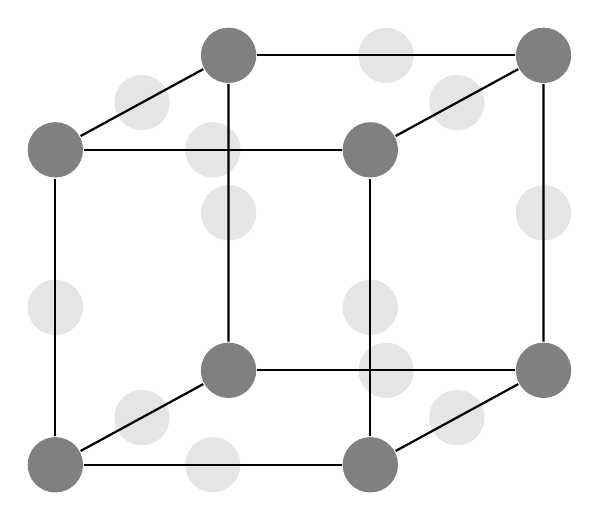
\begin{tikzpicture}[
        scale=2, ->, thick, z={(0.55,0.3)}, node distance=0.65cm, baseline]
        \node[vertex] (v0) at (-1,-1,-1) {};
        \node[vertex] (v1) at (-1,1,-1) {};
        \node[vertex] (v2) at (1,-1,-1) {};
        \node[vertex] (v3) at (1,1,-1) {};
        \node[vertex] (v4) at (-1,-1,1) {};
        \node[vertex] (v5) at (-1,1,1) {};
        \node[vertex] (v6) at (1,-1,1) {};
        \node[vertex] (v7) at (1,1,1) {};
        \node[axial] (c0) at (1,0,-1) {};
        \node[axial] (c1) at (1,0,1) {};
        \node[axial] (c2) at (-1,0,-1) {};
        \node[axial] (c3) at (-1,0,1) {};
        \node[axial] (c4) at (0,1,-1) {};
        \node[axial] (c5) at (0,1,1) {};
        \node[axial] (c6) at (0,-1,-1) {};
        \node[axial] (c7) at (0,-1,1) {};
        \node[axial] (c8) at (-1,-1,0) {};
        \node[axial] (c9) at (-1,1,0) {};
        \node[axial] (c10) at (1,-1,0) {};
        \node[axial] (c11) at (1,1,0) {};
        \draw[edge] (v0) -- (v1) -- (v3) -- (v2) -- (v0);
        \draw[edge] (v0) -- (v4) -- (v5) -- (v1);
        \draw[edge] (v2) -- (v6) -- (v7) -- (v3);
        \draw[edge] (v4) -- (v6);
        \draw[edge] (v5) -- (v7);
        \end{tikzpicture}
        }
        \newline
        \newline
        %\end{adjustbox}
        \caption{Plan factoriel.}
        \label{fig:doe_factorial}
    \end{subfigure}
    \begin{subfigure}[b]{0.32\textwidth}
        \centering
        \resizebox{\linewidth}{!}{
        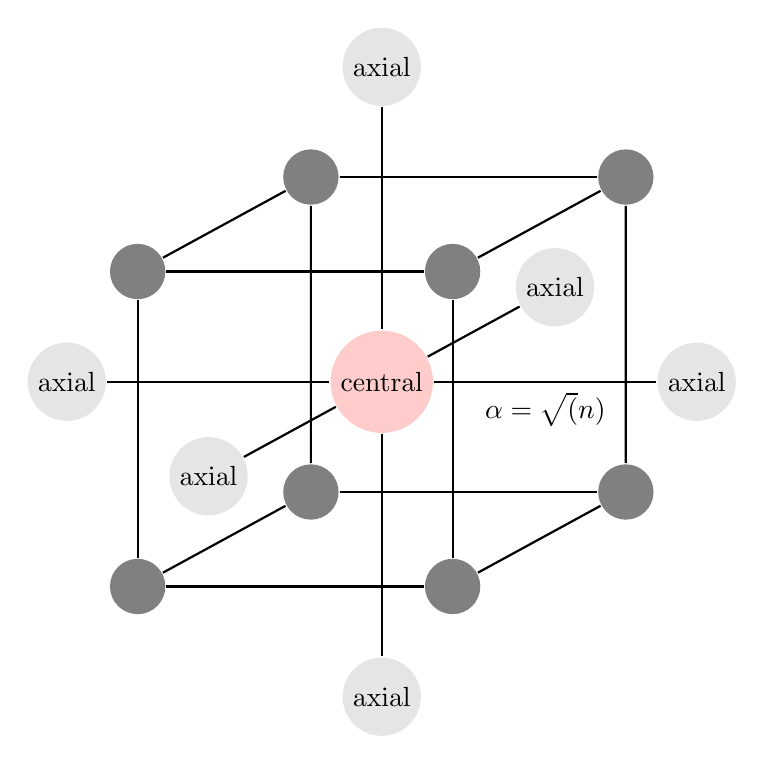
\begin{tikzpicture}[
        scale=2, ->, thick, z={(0.55,0.3)}, node distance=0.65cm]
        \node[vertex, fill=red!20] (c0) at (0,0,0) { \ central \ };
        \node[vertex] (v0) at (-1,-1,-1) {};
        \node[vertex] (v1) at (-1,1,-1) {};
        \node[vertex] (v2) at (1,-1,-1) {};
        \node[vertex] (v3) at (1,1,-1) {};
        \node[vertex] (v4) at (-1,-1,1) {};
        \node[vertex] (v5) at (-1,1,1) {};
        \node[vertex] (v6) at (1,-1,1) {};
        \node[vertex] (v7) at (1,1,1) {};
        \node[axial] (a1) at (-\ax,0,0) { \ axial \ };
        \node[axial] (a2) at (\ax,0,0) { \ axial \ };
        \node[axial] (a3) at (0,-\ax,0) { \ axial \ };
        \node[axial] (a4) at (0,\ax,0) { \ axial \ };
        \node[axial] (a5) at (0,0,-\ax) { \ axial \ };
        \node[axial] (a6) at (0,0,\ax) { \ axial \ };
        \draw[edge] (v0) -- (v1) -- 
        (v3) -- (v2) -- (v0);
        \draw[edge] (v0) -- (v4) -- (v5) -- (v1);
        \draw[edge] (v2) -- (v6) -- (v7) -- (v3);
        \draw[edge] (v4) -- (v6); \draw[edge] (v5) -- (v7);
        \draw[edge] (a1) -- (c0) -- (a2) node[rotu, below=0.1] {$\alpha=\sqrt(n)$};
        \draw[edge] (a3) -- (c0) --(a4);
        \draw[edge] (a5) -- (c0) --(a6);
        \end{tikzpicture}
        }
        \caption{Plan composite centré.}
        \label{fig:doe_cc}
    \end{subfigure}
    \begin{subfigure}[b]{0.30\textwidth}
        \centering
        \resizebox{\linewidth}{!}{
            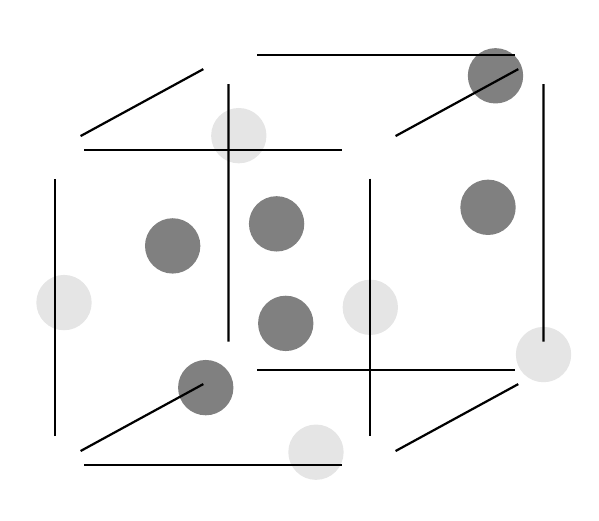
\begin{tikzpicture}[
            scale=2, ->, thick, z={(0.55,0.3)}, node distance=0.65cm]
            \node[empty] (v0) at (-1,-1,-1) {};
            \node[empty] (v1) at (-1,1,-1) {};
            \node[empty] (v2) at (1,-1,-1) {};
            \node[empty] (v3) at (1,1,-1) {};
            \node[empty] (v4) at (-1,-1,1) {};
            \node[empty] (v5) at (-1,1,1) {};
            \node[empty] (v6) at (1,-1,1) {};
            \node[empty] (v7) at (1,1,1) {};
            \node[vertex] (a1) at (-0.20, 0.20, 0.10) {};
            \node[vertex] (a2) at ( 0.75, 0.90, 0.90) {};
            \node[vertex] (a3) at (-0.10,-0.54,-0.90) {};
            \node[vertex] (a4) at (-0.75, 0.12,-0.10) {};
            \node[vertex] (a5) at ( 0.10,-0.30,-0.34) {};
            \node[vertex] (a6) at ( 0.95, 0.20, 0.45) {};
            \node[axial] (c0) at (1,0,-1) {};
            \node[axial] (c1) at (1,-0.9,1) {};
            \node[axial] (c2) at (-1,0,-0.9) {};
            \node[axial] (c3) at (0.6,-0.95,-0.9) {};
            \node[axial] (c4) at (0,1,-0.7) {};
            \draw[edge] (v0) -- (v1) -- (v3) -- (v2) -- (v0);
            \draw[edge] (v0) -- (v4) -- (v5) -- (v1);
            \draw[edge] (v2) -- (v6) -- (v7) -- (v3);
            \draw[edge] (v4) -- (v6);
            \draw[edge] (v5) -- (v7);
            \end{tikzpicture}
        }
        \newline
        \newline
        \caption{Plan hypercube latin.}
        \label{fig:doe_hls}
    \end{subfigure}
    \caption{Essais prévus pour des plans d'expériences à trois niveaux pour trois variables.}
    \label{fig:doe}
\end{figure}

\paragraph{Plan factoriel}\mbox{\label{parag:doe_factorial}} \\
Le \textit{plan factoriel} propose une recherche exhaustive de l'effet de la variation de chacune des variables.
Lorsque la variation des variables est réalisée sur deux niveaux distincts, il permet de construire un modèle linéaire.
Il permet également de rendre compte des interactions entre les variables.
Lorsque la variation des variables est réalisée sur trois niveaux distincts, il permet de construire un modèle quadratique.
Des modèles d'ordre supérieur peuvent être réalisés mais l'augmentation du $k$ nombre d'essais à réaliser suit alors une loi factorielle $2^k$.

\paragraph{Plan central-composite}\mbox{\label{parag:doe_cc}} \\
Le \textit{plan central-composite} (plan de \textit{Box-Wilson}) permet de construire des modèles d'ordre 3.
Il a été proposé dès 1950.
Il s'appuie sur un \textit{plan factoriel} à deux niveaux.
Ce modèle est complété en réalisant des essais pour les valeurs médianes des variables (appelés \textit{essais au centre}).
Enfin, on réalise des essais où chaque variable est ajustée indépendamment des autres (\textit{essais axiaux}).
Un coefficient $\alpha$ définit la valeur de la variation de la variable par rapport à l'essai au centre.
Pour un nombre $n$ de variables à étudier, on choisit généralement $\alpha = \sqrt{n}$.
D'autres méthodes de choix de $\alpha$ sont possibles et nous invitons le lecteur à consulter un ouvrage de référence sur la théorie des plans de surfaces de réponses tel que \cite{myers_response_1971}.
Le \textit{plan central-composite} réduit le nombre d'essais à réaliser en comparaison du \textit{plan factoriel}.
Le plan de \textit{Box-Behnken} propose de réduire le nombre d'essais en n'utilisant pas un plan factoriel comme plan de référence.
% Box-Behnken designs usually have fewer design points than central composite designs, thus, they are less expensive to run with the same number of factors. They can efficiently estimate the first- and second-order coefficients; however, they can't include runs from a factorial experiment. Box-Behnken designs always have 3 levels per factor, unlike central composite designs which can have up to 5. Also unlike central composite designs, Box-Behnken designs never include runs where all factors are at their extreme setting, such as all of the low settings.
Les plans de Plackett-Burman \cite{plackett_design_1946} proposent de réduire le nombre d'essais pour une étude à deux niveaux, dans le cas où le nombre d'essais est un multiple de 4 ($N=12, N=20, N=24 \dots$).
Ces plans sont idéaux pour réaliser une étude de nombreuses variables en peu d'essais et construire un modèle linéaire.

\paragraph{Plan hypercube latin}\mbox{\label{parag:doe_lhs}} \\
L'objectif de ce plan est de couvrir la plage de valeurs des variables de manière quasi-aléatoire.
La méthode de construction de ce plan a été proposée par \cite{mckay_comparison_1979}. % Eglājs in 1977

Soit une grille à deux dimensions qui représente les valeurs de deux variables que l'on étudie.
On positionne sur cette grille des essais.
Cette grille est un \textit{carré latin} si elle ne contient qu'un unique essai par colonnes et par lignes.
Un \textit{hypercube latin} est la généralisation de ce principe pour une grille à $d$ dimensions.
Cette méthode garantit un positionnement quasi-aléatoire des essais dans l'espace de dimensions $d$.
À la différence des plans factoriels §\ref{parag:doe_factorial} ou composite centré §\ref{parag:doe_cc} , le nombre d'essais doit être connu pour construire le plan.
Cette méthode garantit que les essais soient réalisés sur l'ensemble de la variabilité du phénomène à modéliser ; à la différence d'un tirage aléatoire de la valeur des variables où il n'y a pas cette garantie.
Les plans d'hypercubes latins sont les plus utilisés dans la littérature de l'optimisation d'hyper-paramètres.

Il est également possible d'utiliser une séquence quasi-aléatoire pour réaliser le choix des essais.
La séquence de Sobol (\cite{sobol_distribution_1967}) est la plus utilisée dans la littérature.
Lorsque le nombre de variables est inférieur à $100$, il permet une répartition plus intéressante que l'hypothèse des hypercubes latins.
% A Sobol sequence is a low discrepancy quasi-random sequence. Sobol sequences were designed to cover the unit hypercube with lower discrepancy than completely random sampling (e.g. Random Search). Optunity supports Sobol sequences in up to 40 dimensions (e.g. 40 hyperparameters).
% The figures below show the differences between a Sobol sequence and sampling uniformly at random. These figures can be recreated using the code in bin/examples/python/sobol_vs_random.py.
% The mathematical details on Sobol sequences are available in the following papers: [SOBOL], [SOBOL2], [ANTONOV], [BRATLEY], [FOX].
% [SOBOL]   Ilya Sobol, USSR Computational Mathematics and Mathematical Physics, Volume 16, pages 236-242, 1977.
% [SOBOL2]  Ilya Sobol, Levitan, The Production of Points Uniformly Distributed in a Multidimensional Cube (in Russian), Preprint IPM Akad. Nauk SSSR, Number 40, Moscow 1976.
% [ANTONOV] Antonov, Saleev, USSR Computational Mathematics and Mathematical Physics, Volume 19, 1980, pages 252 - 256.
% [BRATLEY] Paul Bratley, Bennett Fox, Algorithm 659: Implementing Sobol’s Quasirandom Sequence Generator, ACM Transactions on Mathematical Software, Volume 14, Number 1, pages 88-100, 1988.
% [FOX] Bennett Fox, Algorithm 647: Implementation and Relative Efficiency of Quasirandom Sequence Generators, ACM Transactions on Mathematical Software, Volume 12, Number 4, pages 362-376, 1986.

% \paragraph{Plan de Taguchi}\mbox{\label{parag:doe_taguchi}} \\
% Bad and/or idocratic

\subsection{Optimisation par méta-modèle bayésien} \label{subsec:bayesian_opt}
% Start with a few (random) hyperparameter confgurations
% • Build a surrogate model to predict how well other confgurations will work: mean and standard deviation (blue band)
% • Any probabilistic regression model: e.g. Gaussian processes
% • To avoid a greedy search, use an acquisition function to trade off
% exploration and exploitation, e.g. Expected Improvement (EI)
% • Sample for the best confguration under that function μ σ H
%
% Repeat
% • Stopping criterion:
% • Fixed budget (time, evaluations)
% • Min. distance between confgs
% • Threshold for acquisition function
% • Still overfts easily
% • Convergence results
% • Good for non-convex, noisy objectives
% • Used in AlphaGo
% 
% Gaussian processes
% + uncertainty, extrapolation
% - Scalability (cubic)
% Sparse GPs[Lawrence et al. 2003]
% Random embeddings [Wang et al. 2013]
% - Robustness? Meta-BayesOpt to optimize kernel [Malkomes et al. 2016]
% Neural networks + Bayesian LR [Snoek et al. 2015]
% + Scalable, Learns basis expansion
% Bayesian neural networks [Springenberg et al. 2016]
% + Bayesian - Scalability not studied yet

Cette démarche cherche dans un premier temps à modéliser le lien entre les hyper-paramètres $\boldsymbol{x}$ et les performances $y = f(\boldsymbol{x}, \boldsymbol{D})$ du modèle $f$ appris sur le jeu de données $\boldsymbol{D}$.
Il s'agit ensuite de résoudre le problème d'optimisation des hyper-paramètres $\boldsymbol{x}$ dans l'espace de valeurs des hyper-paramètres $\mathcal{X}$, afin de trouver les hyper-paramètres optimaux $\boldsymbol{x}_{\star}$.
L'Équation \ref{eq:hp_optimization} présente ce problème dans le cas où la sortie de $f$ est l'erreur d'apprentissage du modèle.

\begin{equation} \label{eq:hp_optimization}
\boldsymbol{x}_{\star} \in \underset{\boldsymbol{x} \in \mathcal{X}}{\arg \min } f(\boldsymbol{x})
\end{equation}

$f$ est approximée par un méta-modèle $\mathcal{M}$, sous la forme de procédés gaussiens \cite{matheron_principles_1963} (cette démarche est aussi appelée \textit{krigeage} \cite{krige_statistical_1951}), qui permet de prendre en compte l'incertitude sur les futures évaluations de $m$, Équation \ref{eq:hp_gp}.
\begin{equation} \label{eq:hp_gp}
y = f(\boldsymbol{x}) \sim \mathcal{M}\left(\mu(\boldsymbol{x}), k\left(\boldsymbol{x}, \boldsymbol{x}^{\prime}\right)\right)
\end{equation}

On cherche à modéliser la distribution de probabilité de $y$ connaissant les hyper-paramètres $\boldsymbol{x}$ : $p(y | \boldsymbol{x})$.
Le procédé gaussien $\mathcal{M}$ est défini par sa moyenne $\mu$ et son noyau $k$ (différents noyaux sont présentés dans la Section précédente §\ref{eq:kernels}).
Le coût de l'optimisation des procédés gaussiens est néanmoins de l'ordre de $\bigO(N^3)$.
L'optimisation de $f$ nécessite généralement de 10 à 100 évaluations de la fonction.
Chaque évaluation de la fonction possède le coût de l'apprentissage du modèle sur le jeu de données complet.
Ce coût est très grand et il est nécessaire de limiter au maximum le nombre d'évaluations du méta-modèle $\mathcal{M}$.
Des modèles différents des coûteux procédés gaussiens ont été proposés.
Nous les présentons dans les Sections suivantes §\ref{subsubsec:rf_opt}, §\ref{subsubsec:tpe_opt}.

Il est également nécessaire de choisir judicieusement les points d'évaluations $\boldsymbol{x}_{n+1}$ de $f$ à la prochaine évaluation.
Il n'est pas judicieux de choisir $\boldsymbol{x}_{n+1} = \mu{x_{n}}$ dans le cas où des minima locaux existeraient.
Le dilemme de l'optimisation itérative apparait : c'est le choix entre l'\textit{exploration} de $f$ pour construire un modèle $\mathcal{M}$ pertinent qui représente tous les minimas (dont le minimum de $f$), et l'\textit{exploitation} des valeurs de $y = f(\boldsymbol{x}_{n+1})$ qui permet d'atteindre le minimum $y_{\star}$ et trouver $\boldsymbol{x}^{\star}$.
Dans le cas de l'optimisation bayésienne, l'\textit{exploration} cherche à choisir un point qui diminuera les régions où l'incertitude du modèle est grande.
C'est pourquoi \cite{jones_efficient_1998} propose le critère de la prédiction de l'amélioration de performance prédite (\textit{Expected Improvement}), Équation \ref{eq:ei}.

 Lors de la prochaine évaluation de $f$, les valeurs $\boldsymbol{x}_{n+1}$ seront choisies pour maximiser ce critère.

\begin{equation} \label{eq:ei}
{EI}_{p(f | D)}\left[\max \left(y_{\star}-f(\boldsymbol{x}), 0\right)\right]
\end{equation}

Cela permet de choisir les valeurs des hyper-paramètres optimales pour l'évaluation suivante de $f$.
D'autres critères, que nous ne pouvons détailler ici, existent.
Ils sont étudiés en réponse aux problèmes de bandits à N bras.
%https://www.cse.wustl.edu/~garnett/cse515t/spring_2015/files/lecture_notes/12.pdf

% SOTA+Monte Carlo: Wilson, James, Frank Hutter, and Marc Deisenroth. “Maximizing acquisition functions for Bayesian optimization.” In Advances in Neural Information Processing Systems, pp. 9906–9917. 2018.

\subsubsection{Forêts d'Arbres décisionnels} \label{subsubsec:rf_opt}
% Random Forests [Hutter et al. 2011, Feurer et al. 2015]
La méthode \textit{SMAC} (\textit{Sequential Model-Based Algorithm Configuration}) est proposée par \cite{hutter_sequential_2011}.
La démarche est identique à la modélisation gaussienne, mais elle utilise ici des Forêts d'Arbres décisionnels (§\ref{parag:random_forests}).
La sélection des premiers essais à réaliser peut être effectuée à partir des plans d'expériences, §\ref{subsec:doe}.
Un plan hypercube latin ou une séquence de Sobol §\ref{parag:doe_lhs} est généralement utilisé.
% F. Hutter. Automated Configuration of Algorithms for Solving Hard Computational Problems. PhD thesis, University of British Columbia, 2009.
% SMAC3:sequential model-based algorithm configuration
% - Factorial
% - Latin Hypercube
% - Sobol
% Frequentist uncertainty estimate (variance)
% + scalable, complex HPs - uncertainty, extrapolation
% Φz P BLR surrogate φz(λ)i (λi,P

% Random Forests (SMAC) example:
La librairie \textit{auto-sklearn} \cite{feurer_efficient_2015} utilise également les Forêts d'arbres décisionnels.
% https://www.kdnuggets.com/2016/10/interview-auto-sklearn-automated-data-science-machine-learning-team.html
% Combined Algorithm Selection and Hyperparameter optimization (CASH):
Elle utilise la majorité des algorithmes de la librairie \textit{Scikit-Learn} \cite{pedregosa_scikit-learn_2011}.
Cela représente la possibilité d'utiliser 15 classifieurs et 14 méthodes de prétraitement des données, ce qui introduit un nombre conséquent de 110 hyper-paramètres.
Cet algorithme utilise un méta-modèle préalablement appris sur un grand nombre de jeux de données, afin de sélectionner les valeurs des hyper-paramètres initiaux.
Cette démarche a été proposée par \cite{feurer_initializing_2015}.
À la manière d'un expert humain qui a appris à prioriser certains algorithmes en fonction du jeu de données auquel il fait face, un méta-modèle est construit sur 140 jeux de données.
Ce méta-modèle permet de sélectionner les hyper-paramètres initiaux en fonction du jeu de données en présence.
Ce travail montre la pertinence du méta-modèle pour la sélection des essais initiaux, en comparaison d'une sélection basée, par exemple, sur un plan latin hypercube §\ref{parag:doe_lhs}.
Enfin, \textit{auto-sklearn} propose de construire un modèle qui agrège plusieurs méthodes différentes en fonction de leurs performances de manière ensembliste §\ref{parag:bagging}.

La Figure \ref{fig:autosk_result} montre le résultat de l'exploration des multiples classifieurs.
Le classifieur le plus performant est ici le \textit{Stochastic Gradient Boosting} §\ref{parag:boosting}, à contrario d'une durée d'apprentissage importante.

\begin{figure}[hbtp]
    \centering
    \includegraphics[width=\textwidth,height=\textheight,keepaspectratio]{../Chap3/Figures/cv_results_images_all.png}
    \caption{Optimisation d'un modèle appris de manière supervisée, à l'aide de la librairie \textit{auto-sklearn} \cite{feurer_efficient_2015}.}
    \label{fig:autosk_result}
\end{figure}


\subsubsection{Estimateur par noyaux structuré en arbre} \label{subsubsec:tpe_opt}
La libraire \textit{hyperopt} \cite{bergstra_making_2013} (\textit{HYPER-parameter OPTimization}) implémente la recherche aléatoire §\ref{subsec:random_search} et l'algorithme \textit{TPE} (\textit{Tree-structured Parzen Estimator}) \cite{bergstra_algorithms_2011} qui réalise une approximation de la fonction $f$ par densité de noyaux (\textit{kernel density estimator}, aussi appelée méthode de Parzen-Rosenblatt).
% initiée par Rosenblatt en 1956 et développée par Parzen en 1962
% Parzen E. (1962). On estimation of a probability density function and mode, Ann. Math. Stat. 33, pp. 1065-1076
% http://jaberg.github.io/hyperopt/
% https://optunity.readthedocs.io/en/latest/index.html
% Cette méthode est parallélisable et produit des résultats équivalents que au critère \textit{Expected Improvements}.
% 1.Test some hyperparameters
% 2. Separate into good and bad hyperparameters (with some quantile)
% 3. Fit non-parametric KDE for and
% 4. For a few samples, evaluate
% Shown to be equivalent to EI!
% Efficient, parallelizable, robust, but less sample efficient than GPs
La modélisation de chaque hyper-paramètre est structurée dans un arbre de recherche.
Le parcours de l'arbre permet de réaliser l'optimisation entre de multiples paramètres.
Une limite forte de cette méthode est que les interactions entre chaque hyper-paramètres ne sont pas prises en compte dans le modèle car chaque hyper-paramètres disposent de leur branche indépendante sur l'arbre.
Dans le cas où deux hyper-paramètres sont inter-dépendants, cette méthode est moins performante que les procédés gaussiens §\ref{subsec:bayesian_opt}.

Dans le cas de l'optimisation bayésienne, on cherche à modéliser la distribution de probabilité de $y$ connaissant les hyper-paramètres $\boldsymbol{x}$ : $p(y | \boldsymbol{x})$.
Dans le cas de l'estimation par densité de noyaux, on cherche à modéliser la distribution de probabilité de $p(\boldsymbol{x} | y)$ et la distribution $p(y)$.
Le théorème de Bayes permet d'obtenir $p(\boldsymbol{x} | y) = p(y) p(y | \boldsymbol{x})$.
À chaque évaluation de $f$, on sépare les combinaisons d'hyper-paramètres qui obtiennent les meilleurs scores $y \le y*$ pour $\boldsymbol{x}^{top}$ et on définit la distribution $m(\boldsymbol{x})=p(\boldsymbol{x}^{meilleurs} | y)$.
Les combinaisons, dont le score est inférieur à $y*$, définissent la distribution $b(\boldsymbol{x})=p(\boldsymbol{x}^{bof} | y)$.
On choisit généralement la limite $y*$ comme le premier quartile, tel que $p(y < y*) = 0.75$.
\cite{bergstra_algorithms_2011} montre que le rapport $m/b$ est équivalent au critère de la prédiction de l'amélioration de performance (§\ref{subsec:bayesian_opt}), ce qui permet de choisir les prochains essais en minimisant $m/b$.

% Dernièrement, la librairie \texitt{HyperOpt-sklearn} [Komer et al. 2019]

\subsection{Méthodes de réduction du coût d'évaluation du méta-modèle} \label{subsec:reduce_opt}
L'évaluation de $f(\boldsymbol{x}, \boldsymbol{D})$ nécessite l'apprentissage d'un modèle sur le jeu de données $\boldsymbol{D}$, ce qui peut prendre plusieurs heures dans le cas de l'utilisation de réseaux de neurones profonds (\textit{Deep Learning} \ref{subsubsec:deep_learning}).
C'est pourquoi des démarches ont récemment été proposées.
% I We often have access to cheap-to-evaluate approximations ˜f(·, b) of the true objective functionf(·), so called fidelities.

\subsubsection{Évaluations partielles des configurations dans une durée limitée} \label{subsubsec:successive_halving}
Dans le cadre des algorithmes bandits, \cite{jamieson_nonstochastic_2015} propose la méthode \textit{Successive Halving} qui permet de réduire le coût de l'optimisation de $f$.
Il s'agit d'évaluer uniquement les configurations d'hyper-paramètres qui présentent un apprentissage de $f$ rapide.
Dans cet objectif, plusieurs évaluations de $f$ sont lancées en parallèle.
Une durée maximale $b$ pour les évaluations est définie.
À la fin de cette durée $b$, l'erreur d'apprentissage de chaque $f$ est évaluée.
La moitié des modèles qui possèdent les erreurs les plus petites est conservée.
La durée maximale $b$ est alors incrémentée et l'évaluation des modèles restants est à nouveau lancée.
Cette démarche est équivalente à l'évaluation itérative de la dérivée de l'erreur d'apprentissage des modèles, tout en étant massivement parallélisable.

Cette méthode s'appuie sur l'hypothèse que le meilleur modèle $f$ aura une vitesse d'apprentissage plus rapide que les autres.
% Régulièrement, au sens des itérations de l'apprentissage, la moitié des modèles qui possèdent les dérivées les plus petites sont arrêtés.
La limite de cette méthode est qu'il y a un risque de ne pas explorer des configurations d'hyper-paramètres qui donneraient de meilleures performances, mais qui sont plus lentes que de mauvaises configurations.
C'est une hypothèse forte qui a été vérifiée dans ce travail sur des bases de données d'apprentissages conséquentes.

\begin{figure}
    \centering
    \begin{subfigure}{.475\textwidth}
        \centering
        \includegraphics[width=\linewidth]{HPS_finished_runs_over_time_images_all.png}
        \caption{Nombre d'évaluations de $f$ réalisées en fonction de la limite de temps $b$.}
        \label{fig:succesive_halving_time}
    \end{subfigure}\hfill% or \hspace{5mm} or \hspace{0.3\textwidth}
    \begin{subfigure}{.485\textwidth}
        \centering
        \includegraphics[width=\linewidth]{HPS_losses_over_time_images_all.png}
        \caption{Erreur lors de l'apprentissage de $f$ en fonction de la limite de temps $b$.}
        \label{fig:succesive_halving_loss}
    \end{subfigure}
    \caption{Évaluation partielle de $f$ en fonction de $b$.}
    \label{fig:succesive_halving}
\end{figure}

La Figure \ref{fig:succesive_halving_time} présente l'évolution du nombre d'évaluations de $f$ en fonction de $b$.
L'augmentation de $b$ limite le nombre d'évaluations de $f$ réalisées.
Il est nécessaire de sélectionner les bonnes configurations d'hyper-paramètres, ce que fait le méta-modèle.
La Figure \ref{fig:succesive_halving_loss} présente l'erreur d'apprentissage de modèles $f$, obtenue pour différentes valeurs de $b$.
L'augmentation de $b$ permet d'augmenter les performances du modèle.
% Often in practice, promising configurations tend to score higher, relatively to the worst ones, even early on in the process.
% There we go! This is what SuccessiveHalving is all about! Here is how the algorithm, makes use of this assumption:
% Randomly sample a set of hyperparameter configurations
% Evaluate the performances of all currently remaining configurations
% Throw out, the bottom half of the worst scoring configurations
% Go back to 2. and repeat until one configuration remains.
% Instead of wasting a lot of training time in configurations that will lead us nowhere, SuccessiveHalving throws as soon as possible. Hence, more training time, i.e. resources, can be allocated to more potentially valuable models.
%
% A huge question when applying SuccessiveHalving, is finding the right trade-off between total ressources and total number of configurations.
% Smaller learning rates often go hand in hand with more resources, more trees in case of (extreme) gradient boosting or more epochs for neural networks.
% How can we tune such a choice? HyperBand proposes a solution, but this one is for next time!

L'utilisation de l'arrêt prématuré §\ref{parag:early_stopping} pendant l'apprentissage de chaque modèle $f$ est également proposée par \cite{domhan_speeding_2015}.
Ce travail introduit l'utilisation d'un modèle prédictif de l'évolution de l'erreur d'apprentissage.
Pour cela, pendant l'apprentissage de $f$, un modèle bayésien (méthode Monte-Carlo par chaînes de Markov) est construit pour prédire l'évolution future de l'erreur d'apprentissage.
Si l'évolution est défavorable, l'apprentissage est stoppé avant la fin du nombre d'itérations prédéfinies.
Dans le cas d'une utilisation de cette méthode pour l'optimisation des hyper-paramètres de réseaux de neurones profonds, les auteurs évaluent le gain à un facteur deux.

\subsubsection{Évaluation de $f$ sur un sous-ensemble des données} \label{subsec:subsampling}
\cite{klein_fast_2016} propose d'évaluer $f$ sur une partition réduite du jeu de données, (cette méthode est appelée \textit{Fabolas}).
La dimension du sous-ensemble du jeu de données est progressivement augmentée au fur et à mesure que des configurations d'hyper-paramètres satisfaisantes sont trouvées.
La vitesse de l'optimisation est augmentée d'un facteur 10 en comparaison d'une optimisation bayésienne ou de la méthode \textit{Hyperband} §\ref{subsec:bandit}.
Associée à l'évaluation partielle par arrêt prématuré, cette méthode est très efficace pour limiter le coût de l'évaluation.

\subsection{Optimisation par algorithmes bandits} \label{subsec:bandit}
% https://medium.com/criteo-labs/hyper-parameter-optimization-algorithms-2fe447525903
% https://maelfabien.github.io/machinelearning/HyperOpt/
Les méthodes bandits à N bras consistent en l'évaluation massivement parallèle de multiples modèles, et en la sélection des meilleurs, à chaque itération.
La méthode \textit{Hyperband} est proposée par \cite{li_hyperband_2016}.
Elle utilise la démarche d'arrêt prématuré de l'apprentissage §\ref{subsubsec:successive_halving}.
% https://openreview.net/forum?id=ry18Ww5ee
L'étude démontre que dans le cas où l'espace des hyper-paramètres est organisé de la pire des façons pour l'algorithme, cela amènera à un coût d'optimisation 5 fois plus grand qu'avec une recherche aléatoire, §\ref{subsec:random_search}, et un coût 10 fois moins grand dans le meilleur cas.
La méthode utilise également l'apprentissage progressif sur des sous-ensembles des données §\ref{subsec:subsampling}.
Les auteurs concluent sur la possibilité d'utiliser les plans d'expériences §\ref{subsec:doe} pour sélectionner les configurations d'hyper-paramètres à évaluer en premier.
% from BOHB:
% Hyperband balances very aggressive evaluations with many configurations on the smallest budget and very conservative runs on the full budget. This helps it guard against having trusted cheap budgets too much.
%
% In practice HB performs very well for small to medium budgets and typically outperforms random search and vanilla BO quite easily in that setting. However, its convergence is limited by its reliance on randomly-drawn configurations: with larger budgets its advantage over random search diminishes. An example of this is given in the plot below.
%

Récemment, la méthode \textit{BOHB} (\textit{Bayesian Optimization and HyperBand}) a été proposée par \cite{falkner_combining_2017, falkner_bohb_2018}.
% http://ais.informatik.uni-freiburg.de/teaching/ws18/deep_learning_lab/presentation_automl.pdf
% Combining Hyperband with Bayesian Optimization [Falkner et al., 2017]
% https://www.automl.org/blog_bohb/
Elle associe les techniques d'\textit{Hyperband} pour la sélection du nombre de configurations à évaluer dans un temps limité, et ajoute l'optimisation d'un méta-modèle bayésien (similaire aux noyaux structurés en arbre \textit{TPE} §\ref{subsubsec:tpe_opt}) pour sélectionner les meilleures configurations à évaluer.
À la différence de \textit{Hyperband} qui sélectionne les configurations de manière aléatoire, le méta-modèle permet de prendre en compte l'information sur les configurations acquise au fur et à mesure des évaluations.
La sélection des configurations à évaluer est plus pertinente, ce qui permet d'atteindre la configuration optimale avec environ deux fois moins d'évaluations que \textit{Hyperband}.
% Hyperband:
% - very efficient in terms of anytime performance
% - due to the random sampling, cannot reuse previously gain knowledge and take a long time to converge
% Bayesian optimization:
% - in its standard form it cannot exploit fidelites (however, several extensions exist)
% - in the most cases converges faster than random search
% Can we combine both methods?
% Bayesian optimization is an efficient strategy for hyperparameter optimization
% BOHB combines Hyperband with Bayesian optimization to combine the strengths of both methods
%
% BOHB combines Bayesian optimization (BO) and Hyperband (HB) to combine both advantages into one, where the Bayesian optimization part is handled by a variant of the Tree Parzen Estimator (TPE; Bergstra et al., 2011) with a product kernel (which is quite different from a product of univariate distributions).  BOHB relies on HB to determine how many configurations to evaluate with which budget, but it replaces the random selection of configurations at the beginning of each HB iteration by a model-based search, where the model is trained on the configurations that were evaluated so far.
%
% BOHB’s strong anytime performance (desideratum 1) stems from its use of Hyperband. Quickly evaluating lots of configurations on small budgets allows BOHB to quickly find some configurations that are promising. The strong final performance (desideratum 2) stems from BOHB’s BO part as the guided search in the end is able to refine the selected configurations.
% 
% The plot at the top of the section shows that BOHB behaves like Hyperband in the beginning and later profits from the constructed BO model. In the beginning, both BOHB and Hyperband show a 20x speedup over  Random Search and standard BO. With increasing budgets, Hyperband’s improvement over Random Search diminishes but BOHB still continues to improve, with a speedup of 55x over Random Search.
% 
% BOAH: A Tool Suite for Multi-Fidelity Bayesian Optimization & Analysis of Hyperparameters
% implements BOHB and analysis
% 
% Monte-Carlo Tree Search
% Pipeline search: Monte Carlo Tree Search
% • Use MCTS to search for optimal pipelines
% • Optimize the structure and hyperparameters simultaneously by building a surrogate model to predict confguration performance
% • Bayesian surrogate model: MOSAIC [Rakotoarison et al. 2019]

Afin d'observer l'influence des différents hyper-paramètres sur la performance du modèle, nous réalisons une analyse de la variance des hyper-paramètres pour $f$ (\textit{ANAVAR}/\textit{ANOVA}), en utilisant la librairie \cite{hutter_efficient_2014}.
Lorsque le nombre d'évaluations du modèle est assez grand ($> 100$), cela permet de rendre compte des interactions possibles entre les hyper-paramètres.
La Figure \ref{fig:fanova} présente les résultats pour deux couples d'hyper-paramètres (\textit{beta} est ici un terme de pénalisation des poids §\ref{parag:weights_decay}).
On observe que les surfaces de réponses sont complexes.
De plus, le nombre d'hyper-paramètres présent est ici de 38 et d'autres interactions existent.
C'est pourquoi un expert humain aurait eu des difficultés à réaliser cette optimisation manuellement, dans un espace continu de dimensions 38.

\begin{figure}
    \centering
    \begin{subfigure}{.49\textwidth}
        \centering
        \includegraphics[width=\linewidth]{fine_beta_2_top_beta_1.png}
        \label{fig:fanova_a}
    \end{subfigure}\hfill% or \hspace{5mm} or \hspace{0.3\textwidth}
    \begin{subfigure}{.49\textwidth}
        \centering
        \includegraphics[width=\linewidth]{fine_beta_2_top_beta_2.png}
        \label{fig:fanova_b}
    \end{subfigure}
    \caption{\textit{fANOVA} des hyper-paramètres suite à l'optimisation avec \textit{BOHB}.}
    \label{fig:fanova}
\end{figure}


\subsection{Optimisation par algorithmes évolutionnistes}
% http://automl.info/tpot/
Proposée en 2016 dans \cite{olson_evaluation_2016, olson_automating_2016}, \textit{TPOT} (\textit{Tree-Based Pipeline Optimization Tool}) s'appuie sur un algorithme génétique pour explorer les configurations d'hyper-paramètres et sur une Forêt d'Arbres décisionnels §\ref{parag:random_forests} pour optimiser le meilleur modèle.
%https://rstudio-pubs-static.s3.amazonaws.com/423824_f67e5db15f6e4e59bcf284208e441cfd.html
% Tree-based pipeline optimization
% • Start with random pipelines, best of every generation will cross-over or mutate
% • GP primitives include data copy and feature joins: trees
% • Multi-objective optimization: accurate but short
% • Easy to parallelize
% • Asynchronous evolution (GAMA)
% copy, change, insert, shrink
%
Nous avons appliqué cette méthode dans \cite{nagorny_polarimetric_2019} sur notre problématique de l'apprentissage supervisé d'un modèle pour le contrôle de la qualité.
Sur des images de dimensions $331 \times 331$ pixels, l'évaluation de 300 modèles $f$ est effectuée en 14 heures.
Le gain de performances suite à l'optimisation des hyper-paramètres est de 2\%.
L'algorithme a trouvé le meilleur modèle possible en une demi-journée.
Un expert humain n'aurait certainement pas réussi à en faire autant aux vues du nombre de modèles différents évalués.
Malgré la durée qui est importante, \textit{TPOT} permet de remplacer une demi-journée d'expertise d'un ingénieur en sciences des données.

%% Dernièrement, l'algorithme GAMA: Gijsbers, Vanschoren 2019
%
% https://deepmind.com/blog/article/population-based-training-neural-networks
% PBT - like random search - starts by training many neural networks in parallel with random hyperparameters. But instead of the networks training independently, it uses information from the rest of the population to refine the hyperparameters and direct computational resources to models which show promise. This takes its inspiration from genetic algorithms where each member of the population, known as a worker, can exploit information from the remainder of the population. For example, a worker might copy the model parameters from a better performing worker. It can also explore new hyperparameters by changing the current values randomly.
% As the training of the population of neural networks progresses, this process of exploiting and exploring is performed periodically, ensuring that all the workers in the population have a good base level of performance and also that new hyperparameters are consistently explored.  This means that PBT can quickly exploit good hyperparameters, can dedicate more training time to promising models and, crucially, can adapt the hyperparameter values throughout training, leading to automatic learning of the best configurations.
%
% CMA-ES : covariance matrix adaptation (CMA), Evolution Strategies

\subsection{Optimisation de l'architecture de réseaux de neurones profonds} \label{subsec:nas}
Afin qu'un modèle à réseaux de neurones profonds soit fonctionnel, son architecture doit être optimisée.
Il est nécessaire d'effectuer une recherche de différentes architectures.
Deux solutions apparaissent : une étude bibliographique des meilleurs modèles proposés sur le problème (aussi appelée \textit{Grad-Student Descent}), ou l'automatisation du processus de recherche (aussi appelée \textit{Neural Architecture Search}), que nous présentons dans la suite.
Le coût de la recherche et de l'optimisation de ces modèles est très important.
C'est pourquoi il est nécessaire de disposer de ressources de calculs conséquentes.
Dans le cas où ces ressources ne sont pas disponibles, on préférera utiliser un apprentissage par transfert de domaine §\ref{subsec:transfer_learning}.

\cite{zoph_neural_2016} propose de réaliser un apprentissage automatique de l'architecture de réseaux profonds.
% This paper addresses the scalability challenge of architecture search by formulating the task in a differentiable manner. Unlike conventional approaches of applying evolution or reinforcement learning over a discrete and non-differentiable search space, our method is based on the continuous relaxation of the architecture representation, allowing efficient search of the architecture using gradient descent. Extensive experiments on CIFAR-10, ImageNet, Penn Treebank and WikiText-2 show that our algorithm excels in discovering high-performance convolutional architectures for image classification and recurrent architectures for language modeling, while being orders of magnitude faster than state-of-the-art non-differentiable techniques.
La méthode permet de proposer l'architecture \textit{NASNet} \cite{zoph_learning_2017} qui établit un nouvel état de l'art en matière de performance de classification sur les jeux de données \textit{ImageNet} et \textit{CIFAR-10} \cite{krizhevsky2009learning}.
Nous avons utilisé la librairie \textit{Auto-Keras} \cite{jin_autokeras_2018} dans \cite{nagorny_polarimetric_2019} sur notre problématique.
Cette méthode propose d'utiliser des architectures de la littérature comme solutions initiales, puis de les modifier progressivement, en utilisant les principes de \cite{zoph_neural_2016}.
Un méta-modèle bayésien §\ref{subsec:bayesian_opt} est construit pour parcourir et optimiser les hyper-paramètres associés.
L'architecture du modèle est contrainte à la dimension de la mémoire du processeur graphique sur lequel le modèle est stocké.
Dans le cas de notre expérimentation, les 11 Giga octets de notre processeur graphique était limitant.
Il n'a pas été possible d'obtenir de meilleures performances suite à l'optimisation.

La recherche d'architecture de réseaux de neurones possède de grands enjeux car il est difficile pour les humains d'inventer des architectures plus performantes, aux vues de leurs complexités grandissantes.
Dernièrement, \cite{elsken_neural_2018} propose un état de l'art exhaustif de la littérature \textit{AutoML}.
Les dernières avancées s'appuient sur l'apprentissage par renforcement pour proposer une recherche d'architecture efficiente.


\subsection{Conclusion : AutoML pour l'industrie}
L'utilisation de solutions d'optimisation automatique de modèles rejoint une double question économique.
Est-il avantageux d'optimiser le modèle pour le procédé industriel ? C'est à dire d'augmenter les performances, par exemple dans le cadre du contrôle de la qualité.
De même, est-il plus coûteux d'optimiser manuellement les hyper-paramètres d'un modèle, ou d'investir dans la puissance de calcul nécessaire à l'automatisation ?
Il est aujourd'hui plus avantageux d'utiliser les méthodes \textit{AutoML}.

% https://github.com/openml/automlbenchmark/blob/master/docs/results.md
Dernièrement, \cite{gijsbers_open_2019} réalise une comparaison de 4 méthodes sur 39 jeux de données.
Ils montrent que sur certaines tâches, l'optimisation n'apporte pas nécessairement de gain en comparaison d'un classifieur à Arbres de Forêts décisionnels.
De plus, les méthode \textit{auto-sklearn} et \textit{TPOT} obtiennent des performances similaires dans la majorité des cas.

Notre problématique industrielle impose des contraintes en matière de puissance de calcul disponible.
C'est pourquoi dans notre cadre, l'optimisation de modèles complexes, tels que les réseaux de neurones profonds, peut être effectuée à une fréquence hebdomadaire.
Le coût d'une optimisation journalière est encore trop conséquent pour être envisagé pour l'industrie de la plasturgie.
Sur des domaines techniques à fortes valeurs ajoutées, le modèle doit avoir les meilleures performances.
Il est alors envisageable d'investir dans de plus grandes infrastructures de calculs afin d'envisager une optimisation journalière.

% Reinforcement Learning
% Meta-RL https://lilianweng.github.io/lil-log/2019/06/23/meta-reinforcement-learning.html

\section{Conclusion : Modélisation par apprentissage pour l'industrie} \label{subsec:conclusion}
Nous avons choisi dans ce chapitre d'étudier une diversité représentative des méthodes et algorithmes existants pour résoudre le problème du contrôle automatique de la qualité.
Maitriser l'ensemble du vaste domaine de l'apprentissage statistique est un processus difficile qui requière plusieurs années.
Les thématiques de l'architecture logicielle, l'application des calculs sur les ressources matérielles, l'efficience des algorithmes et la large thématique de l'optimisation non-convexe sont au cœur de ce domaine.
Dernièrement, la littérature de ce domaine est très dynamique, ce qui rend également difficile le suivi des avancées.
Les moyens de production industrielle ont une inertie beaucoup plus grande que cette littérature, c'est pourquoi il est nécessaire de concevoir des systèmes modulaires, qui pourront être mis à jour, au fur et à mesure des progrès de l'apprentissage statistique.

\paragraph{Contraintes industrielles} \mbox{} \\
Nous avons choisi de proposer une vision globale appliquée à notre problématique industrielle.
Le choix des méthodes et des algorithmes à utiliser dépend fortement des contraintes industrielles.
La Figure \ref{fig:ml_taxonomy} positionne les méthodes présentées dans l'ensemble des méthodes d'apprentissage existantes.
Pour chaque méthode, nous avons discuté du coût des calculs.
C'est une des principales limites au déploiement de solutions d'apprentissage dans l'industrie.
C'est notamment la limite du coût du calcul, en rapport à sa durée, qui est encore aujourd'hui critique.
Nous n'avons pas abordé la problématique de l'utilisation des modèles appris, notamment de la vitesse de l'inférence.
En effet, compte tenu des puissances de calculs disponibles aujourd'hui dans les systèmes embarqués, l'inférence à partir d'images peut être réalisée en quelques millisecondes.
C'est l'apprentissage des modèles et leurs mises à jour, qui sont coûteux.

% TODO: Compare methods : embeddable/on-cloud, cost of computing, model update with respect to industrial process time
% https://ai.stackexchange.com/questions/5728/what-is-the-time-complexity-for-training-a-neural-network-using-back-propagation
\begin{table}[h]
    \centering
    \arrayrulecolor{black}\begin{tabular}{|l|l|l|l|l|l|l|}
        \arrayrulecolor{black}
        %\cline{1-1} \cline{3-6}
        \hhline{---}
        Algorithme  & Complexité & Référence\\
        \hhline{=:=:=:} %\hline
        Machine à vecteurs de support      & $\bigO(N^2)$        & §\ref{parag:svm} \\ \hline
        Réseaux de convolutions & $\bigO(N \ T \ W)$, $T$ nb. itérations, $W$ dim. des poids & §\ref{subsubsec:deep_learning}\\
        \hhline{=:=:=:} %\hline
        Analyse en Composantes Principales & $\bigO(N)$          & §\ref{subsubsec:ACP}\\ \hline
        ACP à noyau                        & $\bigO(N^3)$        & §\ref{subsubsec:kpca}\\ \hline
        \hhline{=:=:=:}
        k-moyennes                         & $\bigO(N \log(N))$  & §\ref{subsubsec:kmeans} \\ \hline
        t-SNE                              & $\bigO(N^2)$        & §\ref{subsubsec:tsne}\\ \hline
        UMAP                               & $\bigO(N \log N)$   & §\ref{subsubsec:umap}\\ \hline
        Auto-encodeur variationnel        & $\bigO(T \ D)$, $T$ nb. itérations, $D$ dim. échantillon  & §\ref{subsubsec:vae}\\ \hline
        Réseaux antagonistes adversaires   & $\bigO(T \ D)$, $T$ nb. itérations, $D$ dim. échantillon & §\ref{subsubsec:GAN}\\ \hline
    \end{tabular}
    \caption{Complexité de l'apprentissage des méthodes étudiées, $N$ nombre d'échantillons.}
    \label{tab:overview}
\end{table}

Le Tableau \ref{tab:overview} synthétise les discussions sur le coût des calculs.
Le choix de la méthode utilisée est dépendant de la fréquence de mise à jour du modèle de la qualité et de la disponibilité des moyens de calculs.
Si les calculs doivent être effectués au plus près de la production, sur des systèmes embarqués, les réseaux de neurones les plus profonds ne sont pas envisageables.
Enfin, il est possible de s'appuyer sur les services de solutions de calculs distribués distantes (\textit{Cloud}), qui limitent la nécessité de maintenance locale des moyens de calculs.
Elle nécessite néanmoins le déploiement d'une infrastructure de réseau informatique fiable.

\paragraph{Vers un modèle robuste de la Qualité} \mbox{} \\
La dernière limite est certainement la plus importante.
Il s'agit du nombre d'échantillons présent dans le jeu de données.
Nous disposons actuellement de jeux de données qui contiennent moins de mille échantillons.
L’état de l’art en \textit{Deep Learning}, nous permet d’envisager la quantité de données nécessaire afin de rendre robuste le système, pour toute machine, avec dix mille pièces dans le jeu de données d’apprentissage (\textit{CIFAR-10} \cite{krizhevsky2009learning} propose 6000 images par classes).

La faisabilité du transfert de la modélisation de la qualité apprise sur une machine, vers une autre machine produisant la même pièce, est en cours d’évaluation.
À terme, cette démarche permettra de réaliser l’apprentissage supervisé de la notion de qualité sur une unique machine, puis de déployer le modèle sur un parc machines complet.
Cela implique que le modèle doit avoir acquis dans sa base d’apprentissage des images prises pour une même pièce, mais dans des configurations de machines différentes.

La littérature renseigne des cas de biais, où le modèle produit des résultats satisfaisants en apparence, alors que le modèle ne s’intéresse pas aux véritables causes.
Dans notre cas, il pourrait s'agir d'une machine qui possède une grille de protection de couleur rouge, qui produirait uniquement des pièces mauvaises, tandis qu’une machine de couleur verte produirait uniquement des pièces bonnes.
Le modèle aura alors généralisé par apprentissage qu’aucune pièce ne pourrait être bonne si produite à côté d’une grille rouge.
Ce résultat sera alors très difficile à comprendre.
L'interprétation des résultats produite par un modèle est un enjeu important.
% http://cedric.cnam.fr/~thomen/cours/MVA/tpuncertainty.html
% Gal uncertainity with Dropout
% [GG16]    Yarin Gal and Zoubin Ghahramani. Dropout as a bayesian approximation: representing model uncertainty in deep learning. In Proceedings of the 33rd International Conference on International Conference on Machine Learning - Volume 48, ICML‘16, 1050–1059. JMLR.org, 2016. URL: http://dl.acm.org/citation.cfm?id=3045390.3045502.
% [GIG17]   Yarin Gal, Riashat Islam, and Zoubin Ghahramani. Deep Bayesian Active Learning with Image Data. In Proceedings of the 34th International Conference on Machine Learning (ICML-17). 2017.
Les visualisations par apprentissage non-supervisé permettent dans notre cas d'identifier des paquets d'échantillons similaires.
Nous obtenons de 4 à 6 classes sur l'étude de la pièce "boite noire", qui correspondent à différents types de défauts.

Enfin, nous pouvons également envisager la construction d’un modèle de qualité qui serait robuste à toutes pièces.
Ce modèle rivaliserait avec l’humain afin de classifier les défauts de n’importe quelle pièce.
Construire ce modèle nécessitera une base de données d’apprentissage supérieure à cent mille pièces (\textit{ImageNet} propose quatorze millions d’images pour vingt mille catégories).
Il nécessiterait aussi un modèle à réseaux de neurones profonds ayant la capacité de prendre en compte ces données.

% Diagramme de Taxonimie
% https://vas3k.com/blog/machine_learning/
% https://tex.stackexchange.com/questions/271170/third-level-organizational-chart-using-latex-tikz/271349#271349
\begin{figure}[htbp]
    \centering
    \hspace*{-5mm}
    \forestset{
        direction switch/.style={
            for tree={
                if level=3{}{draw},
                thick,
                edge={thick},
                if level=1{
                    child anchor=north,
                    edge path={
                        \noexpand\path [\forestoption{edge}] (!u.parent anchor) -- ++(0,-.5em) -| (.child anchor)\forestoption{edge label};
                    },
                    s sep+=.5em,
                    for descendants={
                        child anchor=west,
                        align=left,
                        edge path={
                            \noexpand\path [\forestoption{edge}] (!u.parent anchor) ++(1em,0) |- (.child anchor)\forestoption{edge label};
                        },
                        fit=band,
                    },
                    for tree={
                        parent anchor=south west,
                        anchor=mid west,
                        grow'=0,
                        font=\sffamily,
                        if n children=0{}{
                            delay={
                                prepend={[,phantom, calign with current]}
                            }
                        },
                        before computing xy={
                            l=2em
                        },
                    },
                    before drawing tree={
                        x/.wrap pgfmath arg={##1}{.6*x()},
                        for children={
                            x/.wrap pgfmath arg={##1+1em}{.6*x()},
                            for children={
                                x/.wrap pgfmath arg={##1+2em}{.6*x()},
                            }
                        }
                    }
                }{
                    if level=0{
                        parent anchor=south,
                        anchor=south,
                    }{},
                },
            },
        }
    }
    \begin{forest}
        % forest preamble: determine layout and format of tree
        direction switch
        [Apprentissage statistique
            [Supervisé
                [Traditionnelles
                    [Régression logistique]
                    [Classifieur Bayésien naïf]
                    [Analyse discriminante]
                    [SVM §\ref{parag:svm}]
                    [knn §\ref{parag:knn}]
                    [Bagging §\ref{parag:bagging}]
                    [Arbres de décisions]
                    [Random Forests §\ref{parag:random_forests}]
                    [Boosting §\ref{parag:bagging}]
                    [Réseaux de neurones §\ref{parag:neural_networks}]
                ]
                [Deep Learning
                    [Réseaux de convolutions profonds §\ref{subsubsec:deep_learning}]
                    [Réseaux résiduels §\ref{subsubsec:ResNet}]
                    [Transfert de domaine §\ref{subsec:transfer_learning}]
                    [Réseaux récurrents]
                ]
            ]
            [Semi-supervisé
                [Apprentissage par renforcement]
                [Propagation §\ref{subsubsec:propagation}]
                [SVM à transductions]
                [Multi-instance]
                [Rés. Siamois §\ref{subsubsec:siamese}]
                [Rés. Triplets §\ref{subsubsec:triplet}]
            ]
            [Non-supervisé
                [Apprentissage par renforcement]
                [Factorisation de matrices
                    [ACP §\ref{subsubsec:ACP}]
                    [ACP à noyau §\ref{subsubsec:kpca}]
                    [t-SNE §\ref{subsubsec:tsne}]
                    [Auto-encodeurs §\ref{subsubsec:vae}]
                    [AE. variationnels §\ref{subsubsec:vae}]
                    [GAN §\ref{subsubsec:GAN}]
                ]
                [Graphes de voisinage
                    [k-moyennes §\ref{subsubsec:kmeans}]
                    [Classif. Hiérarchique]
                    [Classif. Spectrale]
                    [Cartes auto-organisatrices]
                    [DBSCAN §\ref{subsubsec:hdbscan}]
                    [HDBSCAN §\ref{subsubsec:hdbscan}]
                    [UMAP §\ref{subsubsec:umap}]
                ]
            ]
        ]
    \end{forest}
    \caption{Taxonomie de l'apprentissage statistique.}
    \label{fig:ml_taxonomy}
\end{figure}